\documentclass{book}
\usepackage{hyperref}
\usepackage{marginnote}
\usepackage{main}
\usepackage{caption}
\usepackage{amsmath,amsthm,amssymb}
\usepackage{mathdots}
\usepackage[svgnames,table,xcdraw]{xcolor}
\usepackage{gettitlestring}
\usepackage{subfiles}
\usepackage{caption}
\usepackage{wrapfig}
\usepackage{yhmath}
\usepackage{xlop}
\usepackage{booktabs}
\usepackage[ruled,vlined]{algorithm2e}
\usepackage{tikz}
\usepackage{graphics}
\usepackage{ragged2e}
\usepackage{blkarray}
\usepackage{boldline,makecell}
\usepackage{chngcntr}
\newtheorem{theorem}{Theorem}[chapter]
\newtheorem{proposition}{Proposition}[chapter]
\newtheorem{lemma}{Lemma}[chapter]
\theoremstyle{plain}
\theoremstyle{definition}
\newtheorem{definition}{Definition}[chapter]
\newtheorem{exm}{\textbf{Example}}
\numberwithin{exm}{chapter}
%\newtheorem{algorithm}{\textbf{Algorithm}}
%\numberwithin{algorithm}{chapter%
%chapter 20
\usepackage{latexsym}
\usepackage{array}

\theoremstyle{remark}
\newtheorem{remark}{\texttt{Remark}}[chapter]

\theoremstyle{summary}
\newtheorem*{smr}{\textbf{Summary}}

\theoremstyle{overview}
\newtheorem*{overview}{\textbf{Overview}}

\newtheorem{problem}{}[chapter]

\newenvironment{example}    % this is the environment name for the input
  {\renewcommand{\qedsymbol}{$\blacksquare$}%
   \pushQED{\qed}\begin{exm}}
  {\popQED\end{exm}}

\newenvironment{summary}    % this is the environment name for the input
  {\renewcommand{\qedsymbol}{$\blacksquare$}%
   \pushQED{\qed}\begin{smr}}
  {\popQED\end{smr}}

\UseRawInputEncoding

\graphicspath{{assets/}}



\begin{document}
		
    \tableofcontents
    
    \chapter*{Grids and Numerical Derivatives}
    \addcontentsline{toc}{chapter}{Grids and Numerical Derivatives}
    
    \section*{Introduction to Python}
    \addcontentsline{toc}{section}{Introduction to Python}
  
    In this course we will use Python to study numerical techniques for solving some partial differential equations that arise in Physics. 
    Don\rq t be scared of this new language. 
    Most of the ideas, and some of the syntax, that you learned for Matlab will transfer directly to Python. 
    We\rq ll work through some brief tutorials about Python at the beginning of eachlab, focusing on the particular ideas that you\rq ll need tocomplete 		    that lab. 
    Pretty soon you will be Python wizards. 
    
    
    \paragraph*{P1.1}
     Work through Chapter 1 of Introduction to Python. There you will learn the basics of how to write a Python program, howtodeclare anduseentities called NumPyarrays, and also learn some basic plotting techniques. 
     With that Python knowledge underourbelts, let\rq s move on to begin our study of partial differential equations.
   

    \section*{Spatial grids}
    \addcontentsline{toc}{section}{Spatial grids}
    
    When we solved ordinary differential equations in Physics 330 we were usually moving something forward in time, so you may have the impression that differential equations always \lq flow\rq .  This is not true. If we solve a spatial differential equation, like the one that gives the shape of a chain draped between two posts, the solution just sits in space; nothing flows. Instead, we choose a small spatial step size (think of each individual link in the chain) and seek to find the correct shape by somehow finding the height of the chain at each link.   
    
    In this course we will solve partial differential equations, which usually means that the desired solution is a function of both space x, which just sits, and time t, which flows. When we solve problems like this we will be using spatial grids, to represent the x-part that doesn\rq t flow. The NumPy arrays that you just learned about above are perfect for representing these kinds of spatial grids. 
    \marginpar{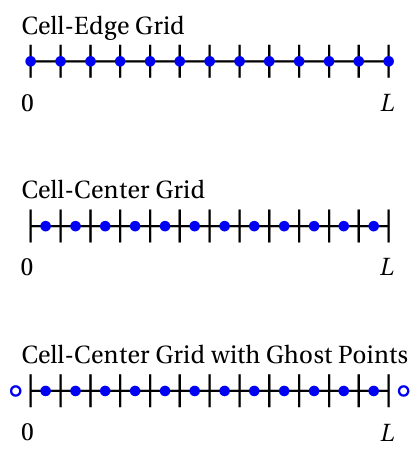
\includegraphics[width=\marginparwidth]{fig1}\captionof{figure}{Three commonspatial grids}}
    
    We\rq ll encounter three basic types of spatial grids in this class. Figure 1.1 shows a graphical representation of these three types of spatial grids for the region 
    \begin{math}0\leqslant x \leqslant l \end{math} . We divide this region into spatial cells (the spaces between vertical lines) and functions are evaluated at N discrete grid points (the dots). In a celledge grid, the grid points are located at the edge of the cell. In a cell-center grid, the points are located in the middle of the cell. Another useful grid is a cell-center grid with ghost points. The ghost points (unfilled dots) are extra grid points on either side of the interval of interest and are useful when we need to consider the derivatives at the edge of a grid.

    \paragraph*{P1.2}
    \begin{enumerate}[label=(\alph*)]
    
      \item  Write a Python program that creates a cell-edge spatial grid in the variable x as follows: 
      \begin{lstlisting}
      	import numpy as np
      	
      	N=100
      	a=0
      	b=np.pi
      	x,h = np.linspace(a,b,N,retstep = True)
 		\end{lstlisting}
      Plot the function y(x) = sin(x)sinh(x) on this grid. Explain the relationship between the number of cells and the numberofgridpoints in a cell-edge grid.

    
    \marginpar{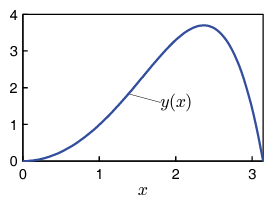
\includegraphics[width=\marginparwidth]{fig2}\captionof{figure}{Plot from 1.2(a)}} 
     
      \item     Explain the relationship between the number of cells and the number of grid points in a cell-center grid. Then write some code using NumPy\rq s arange function to create a cell-centered grid that has exactly 100 cells over the interval 0	$\geq$ x 	$\geq$ 2. 
           \\Evaluate the function f (x)=cosx on this grid and plot this function. Thenestimate the area under the curve by summingtheproductsof the centered function values fj with the widths of the cells h like this (midpoint integration rule):
      
      \begin{lstlisting}
      	np.sum(f)*h
      \end{lstlisting}
      
      Comparethis result to the exact answer obtained by integration: 
      \\      \[A = \int_0^2 cosx \ dx = sin(x) \vert_0^2 = sin(2) \]          
       
\item Build a cell-center grid with ghost points over the interval 0 $\geq$ x $\geq$ $\pi/2$ with 500 cells (502 grid points), and evaluate the function $f (x)=sinx$ on this grid. Now look carefully at the function values at the first two grid points and at the last two grid points. The function sinx has the property that $f(0) = 0$ and $f\prime(\pi/2) = 0$. The cell-center grid doesn\rq t have points at the ends of the interval, so these boundary conditions on the function need to be enforced using more than one point. Explain how the ghost points can be usedinconnectionwith interior points to specify both function-value boundary conditions andderivative-value boundary conditions.	    
    \end{enumerate}  
    
    \marginpar{{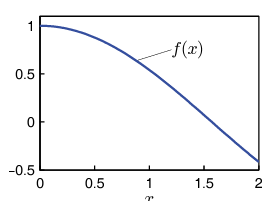
\includegraphics[width=\marginparwidth]{fig3}\captionof{figure}{Plot from 1.2(b)}}}
    
 		\section*{Interpolation and extrapolation}
    \addcontentsline{toc}{section}{Interpolation and extrapolation}   
     
    Grids only represent functions at discrete points, and there will be times when we want to find good values of a function between grid points (interpolation) or beyond the last grid point (extrapolation). We will use interpolation and extrapolation techniques fairly often during this course, so let\rq s review these ideas. Thesimplest way to estimate function values is to use the fact that two points defineastraight line. For example, suppose that we have function values ($x_1$,$y_1$) and ($x_2$,$y_2$). The formula for a straight line that passes through these two points is   
    
\begin{equation} \label{eq:1}
    y - y_1 = \frac{(y_2-y_1)}{(x_2-x_1)}(x-x_1) 
\end{equation}  
  
    Once this line has been established it provides an approximation to the true function $y(x)$ that is pretty good in the neighborhood of the two data points. To linearly interpolate or extrapolate we simply evaluate Eq. \eqref{eq:1} at x values between or beyond $x_1$ and $x_2$.   
      
     \paragraph*{P1.3} UseEq. \eqref{eq:1} to do the following special cases:
     
     \begin{enumerate}[label=(\alph*)]
     
     	\item Find an approximate value for $y(x)$ halfway between the two points $x_1$ and $x_2$. Does your answer make sense?
     	
     	\item Find an approximate value for $y(x)$ 3/4 of the way from $x_1$ to $x_2$. Do you see a pattern?
     	
     \marginpar{{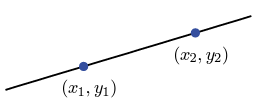
\includegraphics[width=\marginparwidth]{fig4}\captionof{figure}{The line defined bytwo points can be usedtointerpolate betweenthepoints andextrapolate beyond the points.}}}
     
     	\item If the spacing between grid points is h (i.e. $x_2 − x_1 = h$), show that the linear extrapolation formula for $y(x2+h)$ is
     	
     	\begin{equation} \label{eq:2}
     		y(x_2 + h) = 2y_2 - y_1
     	\end{equation}
     	
     	This provides a convenient way to estimate the function value one grid step beyond the last grid point. Also show that
     	
     	\begin{equation} \label{eq:3}
     		y(x_2 + h/2) = 3y_2/2 - y_1/2
     	\end{equation}
     	
     	We will use both of these formulas during the course.
     	
     \end{enumerate}
     \section*{Derivatives on grids}
    \addcontentsline{toc}{section}{Derivatives on grids}  
     
	     Whensolving partial differential equations, we will frequently need to calculate derivatives on our grids. In your introductory calculus book, the derivative was probably introduced using the forward difference formula
		\begin{equation} \label{eg:4}
			f/prime(x) \approx \frac{f(x+h) - f(x)}{h}
		\end{equation}		     
     The word 	$''$ forward	$''$  refers to the way this formula reaches forward from $x$ to $x+h$ to calculate the slope. The exact derivative represented by Eq.\eqref{eg:4} in the limit that h approaches zero. However, wecan\rq t make h arbitrarily small when we represent a function on agrid because $(i)$ the number of cells needed to represent a region of space becomes infinite ash goes to zero; and $(ii)$ computers represent numbers with a finite number of significant digits so the subtraction in the numerator of Eq.\eqref{eg:4} loses accuracy when the two function values are very close. But given these limitation we want to be as accurate as possible, so we want to use the best derivative formulas available. The forward difference formula isn’t one of them.The best first derivative formula that uses only two function values is usually the centered difference formula:
     \begin{equation} \label{eq:5}
     	f\prime(x) \approx \frac{f(x+h)-f(x-h)}{2h} 
     \end{equation}
     It is called $''$centered$''$ because the point x at which we want the slope is centered between the places where the function is evaluated. Take a minute to study Fig. 1.5 to understand visually why the centered difference formula is so much better than the forward difference formula. The corresponding centered second derivative formula is
\marginpar{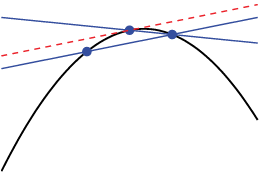
\includegraphics[width=\marginparwidth]{fig5}\captionof{figure}{The forward andcentered difference formulas both approximate the derivative as the slope of a line connecting two points. The centered difference formula gives a moreaccurate approximation because it uses points before and after the point where the derivative is being estimated. (The true derivative is the slope of the dotted tangent line).}}
\begin{equation} \label{eq:6}
	f\prime\prime(x) \approx \frac{f(x+h) - 2f(x)+f(x-h)}{h^2}
\end{equation}
We will derive both of these formulas later, but for now we just want you to understand how to use them. The colon operator provides a compact way to evaluate Eqs. \eqref{eq:5} and \eqref{eq:6} on a grid. Unfortunately for those of you familiar with Matlab, Python$'$ s colon operator acts a little differently from Matlab$'$ s in that the last index is not included in the range, as we noted in the tutorial. If the function we want to take the derivative of is stored in an array f, we can calculate the centered first derivative like this (remember that Python array indexes are zero-based):
\begin{lstlisting}
fp = np.zeros_like(f)
fp[1:N-1]=(f[2:N]-f[0:N-2])/(2*h)
\end{lstlisting}
and the centered second derivative at each interior grid point like this:
\begin{lstlisting}
fpp = np.zeros_like(f) 
fpp[1:N-1]=(f[2:N]-2*f[1:N-1]+f[0:N-2])/h**2
\end{lstlisting}

The variable h is the spacing between grid points and N is the number of grid points. Study this code (focus on the indexing) until you are convinced that it represents Eqs. \eqref{eq:5} and \eqref{eq:6} correctly. \\The derivative at the first and last points on the grid can\rq t be calculated with Eqs.  \eqref{eq:5} and \eqref{eq:6} since there are not grid points on both sides of the endpoints. Instead, we extrapolate the interior values of the two derivatives to the end points. If we use linear extrapolation then we just need two nearby points, and the formulas for the derivatives at the end points are found using Eq. \eqref{eq:2}
\begin{lstlisting}
fp[0]=2*fp[1]-fp[2] 
fp[N-1]=2*fp[N-2]-fp[N-3] 
fpp[0]=2*fpp[1]-fpp[2] 
fpp[N-1]=2*fpp[N-2]-fpp[N-3]
\end{lstlisting}

\paragraph*{P1.4}
Create a cell-edge grid with N = 20 on the interval $0 \leq x \leq 5$. Load $f(x)$ with the Bessel function $J_0(x)$ and numerically differentiate it to obtain $f^\prime(x)$ and $f^\prime\prime(x)$. Then make overlaid plots of the numerical derivatives with the exact derivatives:


\begin{equation*}
\begin{split}
			f^\prime(x) = -J_1(x)\\
			f^{\prime\prime} = \frac{1}{2}(-J_0(x)+J_2(x))	
			\end{split}
\end{equation*}
\marginpar{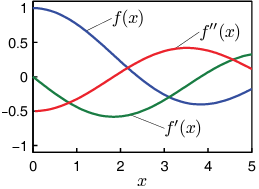
\includegraphics[width=\marginparwidth]{fig6}\captionof{figure}{Plots from 1.4}}

\section*{Errors in the approximate derivative formulas}
\addcontentsline{toc}{section}{Errors in the approximate derivative formulas}  

We\rq ll conclude this lab with a look at where the approximate derivative formulas come from and at the types of the errors that pop up when using them. The starting point is Taylor\rq expansion of the function f a small distance h away from the point x
\begin{equation}\label{eq:7}
	f(x+h) = f(x) + f^\prime(x)h+\frac{1}{2}f^{\prime\prime}(x)h^2 + ... + f^{(n)}(x)\frac{h^n}{n!} + ...
\end{equation}
Let\rq s use this series to understand the forward difference approximation to $f^\prime(x)$. If we apply the Taylor expansion to the $f(x+h)$ term in Eq. \eqref{eg:4} , we get
\begin{equation}\label{eq:8}
\frac{f(x+h) - f(x)}{h}= \frac{[f(x)+f^\prime(x)h+\frac{1}{2}f^{\prime\prime}(x)h^2+...]-f(x)}{h}
\end{equation}
The higher order terms in the expansion (represented by the dots) are smaller than the $f^{\prime\prime}$ term because they are all multiplied by higher powers of h (which we assumetobesmall). If we neglect these higher order terms, we can solve Eq. \eqref{eq:8} for the exact derivative $f^{\prime}(x)$ to find
\begin{equation}\label{eq:9}
f^\prime(x) \approx \frac{f(x+h)-f(x)}{h}-\frac{h}{2}f^{\prime\prime}(x)
\end{equation}
FromEq. \eqref{eq:9} we see that the forward difference does indeed give the first derivative back, but it carries an error term which is proportional to h. But if h is small enough then the contribution from the term containing $f^{\prime\prime}(x)$ will be too small to matter and we will have a good approximation to $f^\prime(x)$. For the centered difference formula, we use Taylor expansions for both $f(x+h)$ and $f(x−h)$in Eq. \eqref{eq:5} to write
\begin{equation} \label{eq:10}
	\frac{f(x+h)-f(x-h)}{2h} = \frac{[f(x)+f^\prime(x)h+f^{\prime\prime}(x)\frac{h^2}{2}+f^{\prime\prime\prime}(x)\frac{h3}{6}+...]}{2h}-\frac{[f(x)-f^\prime(x)h+f^{\prime\prime}(x)\frac{h^2}{2}-f^{\prime\prime\prime}(x)\frac{h3}{6}+...]}{2h}
\end{equation}
If we again neglect the higher-order terms, we can solve Eq. \eqref{eq:10} for the exact derivative $f^\prime(x)$. This time, we find that the $f^{\prime\prime}$ terms exactly cancel to give
\begin{equation} \label{eq:11}
	f^\prime \approx \frac{f(x+h) - f(x-h)}{2h} - \frac{h^2}{6} f^{\prime\prime\prime}(x) 
\end{equation}
Notice that for the centered formula the error term is much smaller, only of order $h^2$. So if we decrease h in both the forward and centered difference formulas by a factor of 10, the forward difference error will decrease by a factor of 10, but the centered difference error will decrease by a factor of 100. This is the reason we try to use centered formulas whenever possible in this course.

\paragraph*{P1.5}
Write a Python program to compute the forward and centered difference formulas for the first derivative of the function $f(x) = e^x $ at $x = 0$ with $h = 0.1, 0.01, 0.001$. Verify that the error estimates in Eqs. \eqref{eq:9} and \eqref{eq:11} agree with the numerical testing. Note that at $x =0$ the exact values of both $f^\prime$ and $f^{\prime\prime}$ are equal to $e^0 = 1$,so just subtract 1 from your numerical result to find the error.

\marginpar{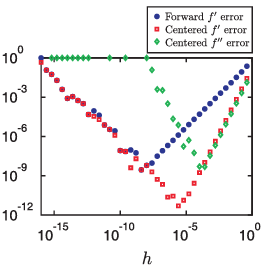
\includegraphics[width=\marginparwidth]{fig7}\captionof{figure}{Error in the forward and centered difference approximations to the first derivative and the centered difference formula for the second derivative as a function of h. Thefunction is $e^x$ and the approximations are evaluated for $x = 0$.}}

In problem 1.5, you found that $h = 0.001$ in the centered-difference formula gives a better approximation than $h=0.01$. This trend might entice you to try to keep making h smaller and smaller to achieve any accuracy you want. This doesn\rq t work. Figure 1.7 shows a plot of the error you calculated in problem 1.5 as h continues to decrease (note the log scales). For the larger values of h, the errors track well with the predictions made by the Taylor\rq s series analysis. However, when h becomes too small, the error starts to increase. By about $h=10−16$, and sooner for the second derivative, the error is the same order as the derivative. Thereason for this behavior is that numbers in computers are represented with a finite number of significant digits. Most computational languages (including Python) use double precision variables, which have 15-digit accuracy.\footnote{A computer uses 64 bits to represent a double precision number. 53 bits are used to represent the significant digits. Thus the significant digit part can be any integer between 0 and 253 = 9007199254740992 (almost 16 digits). The exponent is represented by 11 bits. After you add the possibility of NaN and Inf, the exponent can be −308 to +308. This leaves 1 bit for the overall sign of the number. Extended precision uses more bits (memory) and computation time, so double precision is mostly the standard for computational physics.} This is normally plenty of precision, but look what happens in a subtraction problem where the two numbers are nearly the same:
\begin{equation} \label{eq:12}
\opsub{7.38905699669556}{7.38905699191745}
\end{equation}
Notice that our nice 15-digit accuracy has disappeared, leaving behind only 6 significant figures. This problem occurs in calculations with floating-point numbers on all digital computers, and is called roundoff. You can see this effect by experimenting with the Python console:
\begin{lstlisting}
h=1e-17
g=1+h
print(g-1)
\end{lstlisting}
for different values of h and noting that you don\rq t always get h back. Also notice in Fig. 1.7 that this problem is worse for the second derivative formula than it is for the first derivative formula. The lesson here is that it is impossible to achieve arbitrarily high accuracy by using arbitrarily tiny values of h.
\chapter*{Differential Equations with Boundary Conditions}
\addcontentsline{toc}{chapter}{Differential Equations with Boundary Conditions}  
\section*{More Python}
\addcontentsline{toc}{section}{More Python}  
\paragraph*{P2.1}Work through Chapter 2 of Introduction to Python, where you will learn about lists, loops, and logic.

\section*{Initial conditions vs. boundary conditions}
\addcontentsline{toc}{section}{Initial conditions vs. boundary conditions}  
In Physics 330, we studied the behavior of systems where the initial conditions were specified and we calculated how the system evolved forward in time (e.g. the f light of a baseball given its initial position and velocity). In these cases we were able to use Matlab\rq s convenient built-in differential equation solvers to model the system. The situation becomes somewhat more complicated if instead of having initial conditions, a differential equation has boundary conditions specified at both ends of the interval (rather than just at the beginning). This seemingly simple change in the boundary conditions makes it hard to use canned ODE solvers like Matlab\rq s ode45. Fortunately, there are better ways to solve these systems.

\section*{Solving differential equations with linear algebra}
\addcontentsline{toc}{section}{Solving differential equations with linear algebra} 

Consider the differential equation

\begin{equation} \label{eq:21}
	y^{\prime\prime}(x) + 9y(x) = sin(x) ; y(0) = 0, y(2) = 1
\end{equation}

\marginpar{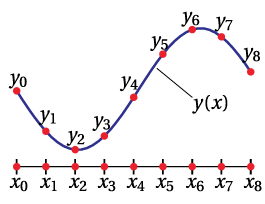
\includegraphics[width=\marginparwidth]{fig8}\captionof{figure}{A function $y(x)$ represented onacell-edge x-grid with $N=9$.}}

Notice that this differential equation has boundary conditions at both ends of the interval instead of having initial conditions at $x = 0$. If we represent this equation on a grid, we can turn this differential equation into a set of algebraic equations that we can solve using linear algebra techniques. Before we see how this works, let\rq s first specify the notation that we\rq ll use. We assume that we have set up a cell-edge spatial grid with N grid points, and we refer to the x values at the grid points using the notation $x_n$, with $n = 0..N−1$. We represent the(as yet unknown) function values $y(xn)$ on our grid using the notation $yn = y(xn)$. Now we can write the differential equation in finite difference form as it would appear on the grid. The second derivative in Eq. \eqref{eq:21} is rewritten using the centered difference formula (see Eq. \eqref{eq:5}), so that the finite difference version of Eq. \eqref{eq:21} becomes:

\begin{equation} \label{eq:22}
	\frac{y_{n+1}-2y_n+y_{n-1}}{h^2}+9y_n = sin(x_n)
\end{equation}


Now let\rq s think about Eq.\eqref{eq:22} for a bit.First notice that it is not an equation, but a system of many equations.We have one of these equations at every grid point n, except the end points j=0 and at j=N−1 where this formula reaches beyond the ends of the grid and cannot,therefore,be used.Because this equation involves $y_{n−1}$,$y_n$,and $y_{n+1}$ for the interior grid points n=1...N−2, Eq.(2.2) is really a  system of N−2 coupled equations in the N unknowns $y_0$ ...$y_{N−1}$.If we had just two more equations we could find the $y_n$\rq s by solving a linear system of equations. But we do have two more equations; they are the boundary conditions:
\begin{equation} \label{eq:23}
	y_0 = 0 ; y_{N-1} = 1
\end{equation}

which completes our system of N equations in N unknowns.\\
 Before Python can solve this system we have to put it in a matrix equation of the form

\begin{equation} \label{eq:24}
	A_y=b,
\end{equation}
where A is a matrix of coefficients, y the column vector of unknown y-values, and b the column vector of known values on the right-hand side of Eq.\eqref{eq:22}.For the particular case of the system represented by Eqs.\eqref{eq:22} and \eqref{eq:23} ,the matrix equation is given by


\begin{equation} \label{eq:25}
	\begin{bmatrix}
		1 & 0 & 0 & 0 & ... & 0 & 0 & 0 \\
		\frac{1}{h^2} & -\frac{2}{h^2}+9 & \frac{1}{h^2} & 0 & ... & 0 & 0 & 0 \\
		0 &\frac{1}{h^2} & -\frac{2}{h^2}+9 & \frac{1}{h^2} & ... & 0 & 0 & 0 \\
		. & . & . & . & ... & .& . &. \\
		. & . & . & . & ... & .& . &. \\
		. & . & . & . & ... & .& . &. \\
		0 & 0 & 0 & 0 & ... & \frac{1}{h^2} & -\frac{2}{h^2}+9 & \frac{1}{h^2} \\
		0 & 0 & 0 & 0 & ... & 0 & 0 & 1  \\
	\end{bmatrix}
	\begin{bmatrix}
	y_0 \\ 
	y_1 \\ 
	y_2 \\ 
	. \\
	. \\
	. \\
	y_{N-2} \\ 
	y_{N-1} \\ 
	\end{bmatrix}
	=
	\begin{bmatrix}
		0 \\ 
		sin(x_1) \\
		sin(x_2) \\
		. \\
		. \\
		. \\
		sin(x_{N-2}) \\
		1 \\
	\end{bmatrix}
\end{equation}

Convince yourself that Eq.\eqref{eq:25} is equivalent to Eqs. \eqref{eq:22} and  \eqref{eq:23} by mentally doing each row of the matrix multiply by tipping one row of the matrix up on end,dotting it into the column of unknowny-values, and setting it equal to the corresponding element in the column vector on the right. Once we have the finite-difference approximation to the differential equation in this matrix form $(Ay=b)$, a simple linear solve is all that is required to find the solution array $y_n$. NumPy can do this solve with the command linalg.solve(a,b).

\paragraph*{P2.2}
\begin{enumerate}[label=(\alph*)]
	\item  Setup a cell-edge grid with $N=30$ grid points, like this: 
	\begin{lstlisting}	
	import numpy as np 
	N=30     #thenumberofgridpoints 
	a=0 
	b=2 
	x,h=np.linspace(a,b,N,retstep=True)
	\end{lstlisting}	
	 Look over this code and make sure you understand what it does before just using it.
	\item If you solve Eq. \eqref{eq:21} analytically, you find
	\begin{equation}
	y(x) = \frac{16sin(3x)+cos(6-x)-cos(6+x)+cos(2+3x)-cos(2-3x)}{16sin(6)}
\end{equation}		
		Type this solution formula into the Python program that defines the grid above andplot the exact solution as a blue curve on a cell-edge grid with N points.
\marginpar{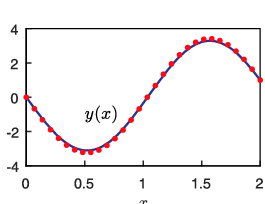
\includegraphics[width=\marginparwidth]{fig9}\captionof{figure}{The solution to 2.2(c) with N = 30}}

		\item Now create a matrix A filled with zeros using np.zeros, and write a for loop to load A like the matrix in Eq. \eqref{eq:25} and do the linear solve to obtain $y_n$ and plot it on top of the exact solution with red dots ('r.') to see how closely the two agree. Experiment with larger values of N and plot the difference between the exact and approximate solutions to see how the error changes with N. We think you\rq ll be impressed at how well the numerical method works, if you use enough grid points.
\end{enumerate}

Let\rq s pause a moment to review how to apply this technique to solve a problem. First, write out the differential equation as a set of finite difference equations on a grid, as we did in Eq. \eqref{eq:22}. Then translate this set of finite difference equations (plus the boundary conditions) into a matrix form analogous to Eq. \eqref{eq:25}. Finally, build the matrix A and the column vector y in Python and solve for the vectory. Our example, Eq. \eqref{eq:21}, had only a second derivative, but first derivatives can be handled using the centered first derivative approximation, Eq. \eqref{eq:5}. Let\rq s practice this procedure for a couple more differential equations:
\paragraph*{P2.3}
	\begin{enumerate}[label=(\alph*)]
		\item Write out the finite difference equations on paper for the differential equation
		\marginpar{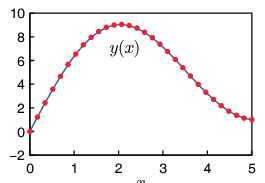
\includegraphics[width=\marginparwidth]{fig10}\captionof{figure}{Solution to 2.3(a) with N =30 (dots) compared to the exact solution (line)}}
		\begin{equation} \label{eq:26}
				y^{\prime\prime} + \frac{1}{x}y^\prime + (1 - \frac{1}{x^2})y=x ; y(0) = 0 , y(5) = 1
		\end{equation}
		Then write down the matrix A and the vector b for this equation. Finally, build these matrices in a Python program and solve the equation using the matrix method. Compare the solution found using the matrix method with the exact solution
		\begin{equation*}
			y(x) = \frac{-4}{J_1(5)}J_1(x)+x
		\end{equation*}
		$J_1(x)$ is the first order Bessel function.\\ HINT: When creating your b vector, you\rq ll be tempted to write some code like this: $b=x$. Don\rq t. This code just assigns b to be a reference to the matrix x. What you want is to create a copy of the matrix like this: \\ 
		\begin{lstlisting}	
	b = np.copy(x)
	\end{lstlisting}
	\item 	Solve the differential equation
	\begin{equation}\label{eq:27}
	y^{\prime\prime} + sin(x)y^\prime+e^xy=x^2 ; y(0) = 0, y(5)=3
\end{equation}		
	in Python using the matrix method. Mathematica\rq s NDSolve command claims that, to 15-digit accuracy
		\begin{equation*}
			y(4.5) = 8.720623277763513
		\end{equation*}

		\marginpar{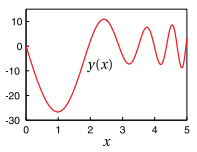
\includegraphics[width=\marginparwidth]{fig24}\captionof{figure}{Solution to 2.3(b) with N = 200}}
	You\rq d run out of memory with the matrix method long before achieving this level of accuracy, but how many points do you have to use in your numerical method to get agreement with Mathematica to 3 digits of accuracy (i.e. $y(4.5) = 8.72$)?		
		\\
		Hint: If your step size variable is h, the index for the for element where
$x_j \approx 4.5$ can be found this way:
	\begin{lstlisting}
		j = int(4.5/h)
	\end{lstlisting}
	The int command rounds the result and casts it as an integer so you can use it to access a specific element.
	\end{enumerate}
	
\section*{Derivative boundary conditions}
\addcontentsline{toc}{section}{Derivative boundary conditions} 
	Now let\rq s see how to modify the linear algebra approach to differential equations
so that we can handle boundary conditions where derivatives are specified instead
of values. Consider the differential equation
	\begin{equation}\label{eq:28}
		y^{\prime\prime}(x) + 9y(x) = x   ;    y(0) = 0,    Y^\prime(2) = 0
	\end{equation}
	We can satisfy the boundary condition $y(0) = 0$ as before (just use $y_1 = 0$), but
what do we do with the derivative condition at the other boundary?
\paragraph*{P2.4}
	\marginpar{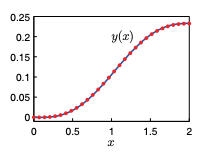
\includegraphics[width=\marginparwidth]{fig25}\captionof{figure}{The solution to $2.4$ (a) with $N=30$. The RMS difference from the exact solution is $8.8 \times 10^{-4}$}}
\begin{enumerate}[label=(\alph*)]
\item	A crude way to implement the derivative boundary condition is to use a forward difference formula for the last two points:
	\begin{equation*}
		\frac{y_{N-1}-y_{N-2}}{h} = y^\prime\vert_{x=2}
	\end{equation*}
	In the present case, where $y^\prime(2) = 0$, this simply means that we need to write the last row of our matrix to enforce
	\begin{equation*}
		y_{N-1}-y_{N-2}= 0
	\end{equation*}
	Think about what the new boundary conditions will do to the final row of matrix A and the final element of vector b, and then solve Eq. \eqref{eq:28} using the matrix method with this boundary condition. Compare the resulting numerical solution to the analytic solution:
	\begin{equation*}
		y(x) = \frac{x}{9} - \frac{\sin(3x)}{27\cos(6)}
	\end{equation*}
	\item You can improve the boundary condition formula using quadratic extrapolation. In this method, you fit a parabola of the form
	\begin{equation}\label{eq:29}
		y(x) = a+bx+cx^2
	\end{equation}
	to the last three points on your grid to find a, b, and c in terms of your data points. Then you take the derivative of Eq. \eqref{eq:28} and evaluate it at
the edge $x = x_{N−1}$. Normally we\rq d make you go through the math to
derive this, but since time is short, we\rq ll just tell you that this process
gives you the following finite difference approximation for the $y^\prime(x)$ at
the end of the grid:
	\begin{equation}\label{eq:210}
		\frac{1}{2h} y_{N-3} - \frac{2}{h} y_{N-2} + \frac{3}{2h} y_{N-1} = y^\prime(X_{N-1})
	\end{equation}
		\marginpar{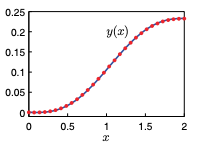
\includegraphics[width=\marginparwidth]{fig26}\captionof{figure}{The solution to $2.4$ (b) with $N=30$. The RMS difference from the exact solution is $5.4 \times 10^{-4}$}}
Modify your program from part (a) to include this new condition and
show that it gives a more accurate solution than the crude technique of
part (a). When you check the accuracy, don\rq t just look at the end of the
interval. All of the points are coupled by the matrix A, so you should
use a full-interval accuracy check like the RMS (root-mean-square)
error:
\begin{lstlisting}
np.sqrt(np.mean((y-yexact)**2))
\end{lstlisting}
\end{enumerate}

\section*{Nonlinear differential equations}
\addcontentsline{toc}{section}{Nonlinear differential equations} 
Finally, we must confess that we have been giving you easy problems to solve,
which probably leaves the impression that you can use this linear algebra trick
to solve all second-order differential equations with boundary conditions at the
ends. The problems we have given you so far are easy because they are linear
differential equations, so they can be translated into linear algebra problems.
Linear problems are not the whole story in physics, of course, but most of the
problems we will do in this course are linear, so these finite-difference and matrix
methods will serve us well in the labs to come.
	\marginpar{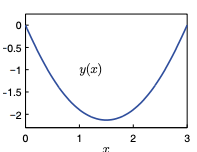
\includegraphics[width=\marginparwidth]{fig27}\captionof{figure}{The solution to $2.5(\mathrm{~b})$.}}
\paragraph*{P2.5}
\begin{enumerate}[label=(\alph*)]
\item Here is a simple example of a differential equation that isn\rq t linear:

	\begin{equation}\label{eq:211}
		y^{\prime\prime}(x) + \sin[y(x)] = 1 ; y(0) = 0, y(3) = 0
	\end{equation}
		Work at turning this problem into a linear algebra problem to see why
it can\rq t be done, and explain the reasons to the TA.
\item Let\rq s find a way to use a combination of linear algebra and iteration
(initial guess, refinement, etc.) to solve Eq. \eqref{eq:211} in Python on a grid.
First, write the equation as
\begin{equation}\label{eq:212}
		y^{\prime\prime}(x)= 1 - \sin[y(x)]
	\end{equation}
	Make a guess for $y(x)$. It doesn\rq t have to be a very good guess. In this
case, the guess $y(x) = 0$ works just fine. Then treat the whole right side
of Eq.\eqref{eq:212} as known so it goes in the b vector. Then you can solve the equation to find an improved guess for
$y(x)$. Use this better guess to rebuild b (again treating the right side of Eq. \eqref{eq:212} as known), and
then re-solve to get and even better guess. Keep iterating until your $y(x)$ converges to the desired level of accuracy. This happens when your $y(x)$  satisfies \eqref{eq:212}  to a specified criterion, not when the change
in $y(x)$ from one iteration to the next falls below a certain level. Iterate until your RMS error is less than $10^{-5}$, as described in the hint below.
HINT: An appropriate error vector would be
\begin{lstlisting}
err = A@y-(1-np.sin(y))
\end{lstlisting}
(remember that @ is the matrix multiplication operator). Compare
this to Eq. \eqref{eq:212}
 and convince yourself that the entire vector err will
be zero when the equation is exactly solved. We\rq ll compute the RMS
error at interior points only, like this
\begin{lstlisting}
rmserr = np.sqrt(np.mean(err[1:-2]**2))
\end{lstlisting}
because the end points don\rq t satisfy the differential equation. Use rmserr as your check condition.
\end{enumerate}

\chapter*{The Wave Equation: Steady State and Resonance}
\addcontentsline{toc}{chapter}{The Wave Equation: Steady State and Resonance} 
\section*{Python Mechanics}
\addcontentsline{toc}{section}{Python Mechanics} 

\paragraph*{P3.1} Work through Chapter 3 of Introduction to Python, where you will learn
about user-defined functions and good commenting practices. For the
remainder of the course, you will need to demonstrate good commenting
practices in your code before your exercises will be passed off.
\section*{Wave Equation}
\addcontentsline{toc}{section}{Wave Equation} 

We are now ready to tackle our first partial differential equation: the wave equation. For a string of length L fixed at both ends with a force applied to it that varies
sinusoidally in time, the wave equation can be written as


\begin{equation}\label{eq:31}
		\mu \frac{\partial^2 y}{\partial t^2} = T \frac{\partial^2y}{\partial x^2} + f(x) \cos \omega t ; y(0,t) = 0, y(L,t) = 0
				\end{equation}
				
		where $y(x,t)$ is the lateral displacement of the string as a function of position
and time, assuming that $y(x,t) ≪ L.$
1 We have written Eq. \eqref{eg:31} in the form of
Newton\rq s second law, $F = ma$. The “ma” part is on the left of the equation, except
that $\mu$ is not the mass, but rather the linear mass density (mass per length). This
means that the right side should have units of force/length, and it does because
T is the tension (force) in the string and $\partial^2y / \partial x^2$
 has units of 1/length. Finally,
$f (x)$ is the amplitude of the driving force (in units of force/length) applied to the
string as a function of position (so we are not necessarily just wiggling the end of
the string) and ω is the frequency of the driving force. \\
Before calculating, let\rq s train our intuition to guess how the solutions of this
equation behave. If we suddenly started to push and pull on a string under tension
with force density $f(x)\cos(\omega t)$, we would launch traveling waves, which would
reflect back and forth on the string as the driving force continued to launch more
waves. The string motion would rapidly become very messy. But suppose that
there is a bit of damping in the system (not included in the equation above, but in
Lab 5 we will add it). With damping, all of the transient waves due to the initial
launch and subsequent reflections would die away and we would be left with a
steady-state oscillation of the string at the driving frequency $\omega$. This behavior is
the wave equation analog of damped transients and the steady final state of a
driven harmonic oscillator which you studied in Physics 330.		

\section*{Steady state solution by separation of variables}
\addcontentsline{toc}{section}{Steady state solution by separation of variables} 
Let\rq s look for this steady-state solution by guessing that the solution has the form
\begin{equation}\label{eq:32}
		y(x,t) = g(x)\cos(\omega t)
				\end{equation}
				This function has the form of a spatially dependent amplitude $g (x)$ which oscillates in time at the frequency of the driving force. Substituting this \lq\lq guess \rq\rq into the
wave equation and carrying out the derivatives yields (after some rearrangement)
\begin{equation}\label{eq:33}
		Tg^{\prime\prime}(x) + \mu \omega ^ 2 g(x) = -f(x) ; g(0) = 0, g(L) = 0
				\end{equation}
				This is just a two-point boundary value problem of the kind we studied in Lab 2,
so we can solve it using our matrix technique.
\paragraph*{P3.2}
	\marginpar{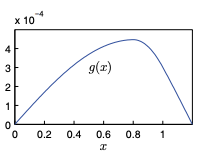
\includegraphics[width=\marginparwidth]{fig31}\captionof{figure}{Solution to P3.2(a)}}
\begin{enumerate}[label=(\alph*)]
	\item Write a program to solve Eq. \eqref{eg:33} for $N = 100$ points with $ \mu = 0.003,
T = 127, L = 1.2$, and $\omega = 400$. All quantities are in SI units. Find the
steady-state amplitude associated with the driving force density:
\begin{equation}\label{eq:34}
		f(x) = 
		\begin{cases}
		0.73 \ if \ 0.8 \	\geq x 	\geq 1 \\
		0 \ \ otherwise
		\end{cases}
				\end{equation}which is something like grabbing the string toward one end and wiggling. Plot $g(x)$, and properly label the axes of your plot.
				\item Take your code from (a) and turn it into a library with two functions:
				\begin{enumerate}
				\item	A function force that accepts the grid $x$ as an argument and
returns the column vector representing $f(x)$

\item A function $steadySol$ that accepts the arguments $f(x)$ (returned
from force), $h$, $\omega$, $T$ , and $\mu$. This function should construct the
matrix, solve the matrix equation, and return $g(x)$.
\end{enumerate}

	\marginpar{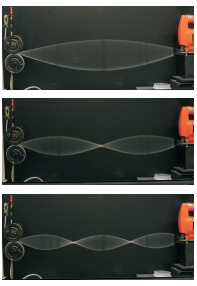
\includegraphics[width=\marginparwidth]{fig32}\captionof{figure}{Photographs of the first three resonant modes for a string fixed at both ends.}}
Save this library as “Lab3Funcs.py” and then write another program
that imports this library. In this program, write a $for$ loop that sweeps
the value of $\omega$ from $\omega = 400$to $\omega = 1700$ in 200 steps keeping the
values of the other parameters constant. Plot $g(x)$ at each frequency
so that you make an animation of what happens when you sweep the
driving frequency. Here is some example code to help you make the
animation, assuming you\rq ve stored your ω values in wplot:
		\begin{lstlisting}
		plt.figure(1)
for n in range(len(wplot)):
w = wplot[n]
g = l3.steadySol(f,h,w,T,u)
plt.clf() # Clear the previous plot
plt.plot(x,g)
plt.title('$\omega={:1.2e}$'.format(w))
plt.xlabel('x')
plt.ylim([-0.05, 0.05]) # prevent auto-scaling
plt.draw() # Request to draw the plot
plt.pause(0.1) # Allow time to draw it
		
\end{lstlisting}
	\marginpar{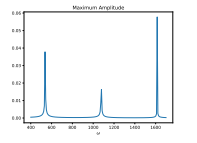
\includegraphics[width=\marginparwidth]{fig33}\captionof{figure}{Solution to problem 3.2(c).}}
At certain frequencies, you should see distinct resonance modes appear as in Fig. 3.2.
\item Modify your code from part (b) so that you find and record the maximum amplitude of $g(x)$ at each $\omega$. Then plot the maximum amplitude
as a function of ω to see the resonance behavior of this system. Describe what the peaks in this plot mean.
				
				
\end{enumerate}
				The height of the peaks in this Fig. 3.3 isn\rq t meaningful—the height of the
actual peak is essentially infinite (since we don’t have any damping yet), while
the height displayed on the plot is just a reflection of how closely our chosen
frequencies happened to line up with the exact resonance frequency. Now we will
learn how to find these resonant frequencies directly without needing to solve
the differential equation over and over again.

\section*{Resonance and the eigenvalue problem}
\addcontentsline{toc}{section}{Resonance and the eigenvalue problem} 
The essence of resonance is that at certain frequencies a large steady-state amplitude is obtained with a very small driving force. To find these resonant frequencies
we seek solutions of Eq. \eqref{eq:33} for which the driving force is zero. With $f(x) = 0$,
Eq. \eqref{eq:33} takes on the form

\begin{equation}\label{eq:35}
		Tg^{\prime\prime}(x) + \mu \omega ^ 2 g(x) = 0 \ ; \ g(0) = 0, g(L) = 0
				\end{equation}
				If we rewrite this equation in the form
				\begin{equation}\label{eq:36}
		g^{\prime\prime}(x) = - (\frac{\mu \omega^2}{T}g(x)
				\end{equation}
				
				\begin{equation}\label{eq:37}
		Ag =\lambda g
				\end{equation}
				where A is a linear operator (the second derivative on the left side of Eq. \eqref{eg:36} )
and $\lambda$ is the eigenvalue $(−\mu \omega^2 / T )$.
Equation \eqref{eg:36} is easily solved analytically, and its solutions are just the familiar
sine and cosine functions. The boundary condition $g (0) = 0$ tells us to try a sine
function form, $g (x) = g_0 \sin(kx)$. If we substitute this form into Eq. \eqref{eg:36} , we find
that it works, provided that k satisfies k = $\omega \sqrt{\frac{\mu}{ T}}$ . We the have
		\begin{equation}\label{eq:38}
		g(x) = g_0\sin(\omega \sqrt{\frac{\mu}{T}x})
				\end{equation}		
				where $g_0$ is the arbitrary amplitude. When we apply the boundary condition
$g(L) = $0, we find that the resonant frequencies take on discrete values given by
\begin{equation}\label{eq:39}
		\omega = n \frac{\pi}{L}\sqrt{\frac{T}{\mu}}
				\end{equation}	
				where $n$ is an integer. Each value of $n$ gives a specific resonance frequency from
Eq. \eqref{eg:39} and a corresponding spatial mode $g(x)$ given by Eq. \eqref{eg:38}
For this simple example we were able to do the eigenvalue problem analytically, but when the differential equation is not so simple we will need to do the
eigenvalue calculation numerically. Let\rq s see practice the numerical calculations
in this case where we know the answer. Rewriting Eq. \eqref{eg:35} in matrix form using
finite differences, as we learned to do in the last lab, yields
\begin{equation}\label{eq:310}
		Ag = \lambda g
				\end{equation}
				where $ \lambda = - \mu\omega^2/T$. With finite differencing, this becomes the matrix equation
				\begin{equation}\label{eq:311}
\left[\begin{array}{cccccccc}
? & ? & ? & ? & \ldots & ? & ? & ? \\
\frac{1}{h^{2}} & -\frac{2}{h^{2}} & \frac{1}{h^{2}} & 0 & \ldots & 0 & 0 & 0 \\
0 & \frac{1}{h^{2}} & -\frac{2}{h^{2}} & \frac{1}{h^{2}} & \ldots & 0 & 0 & 0 \\
\cdot & \cdot & \cdot & . & \ldots & . & . & \cdot \\
\cdot & . & . & . & \ldots & . & \cdot & \cdot \\
. & . & . & . & \ldots & . & \cdot & \dot{1} \\
0 & 0 & 0 & 0 & \ldots & \frac{1}{h^{2}} & -\frac{2}{h^{2}} & \frac{1}{h^{2}} \\
? & ? & ? & ? & \ldots & ? & ? & ?
\end{array}\right]\left[\begin{array}{r}
g_{0} \\
g_{1} \\
g_{2} \\
\cdot \\
\cdot \\
\cdot \\
g_{N-2} \\
g_{N-1}
\end{array}\right]=\lambda\left[\begin{array}{r}
? \\
g_{1} \\
g_{2} \\
\cdot \\
\cdot \\
\cdot \\
g_{N-2} \\
?
\end{array}\right]
\end{equation}
The question marks in the first and last rows remind us that we have to invent
something to put in these rows to implement the boundary conditions. The
answer we are seeking is the function $g$, and it appears on both sides of the
equation. Thus, the question marks in the
g -vector on the right are a real problem
because without
$g_0$ and
$g_{N-1}$, we don\rq t have an eigenvalue problem (i.e.
$g$ on left
side of Eq. \eqref{eg:311} is not the same as
$g$ on the right side). \\ 
The simplest way to deal with this question-mark problem and to also handle
the boundary conditions is to change the form of Eq. \eqref{eg:37} to the slightly more
complicated form of a generalized eigenvalue problem, like this:
\begin{equation}\label{eq:312}
		Ag = \lambda Bg
				\end{equation}

where $B$ is another matrix, whose elements we will choose to make the boundary
conditions come out right. To see how this is done, here is the generalized modification of Eq. \eqref{eg:311} with $B$ and the top and bottom rows of A chosen to apply the boundary conditions
$g (0) = 0$ and $g(L)= 0$:
\begin{equation}
\left[\begin{array}{cccccc}
1 & 0 & 0 & \cdots & 0 & 0 \\
\frac{1}{h^{2}} & -\frac{2}{h^{2}} & \frac{1}{h^{2}} & \cdots & 0 & 0 \\
0 & \frac{1}{h^{2}} & -\frac{2}{h^{2}} & \cdots & 0 & 0 \\
\cdot & \cdot & \cdot & \cdots & \cdot & \cdot \\
\cdot & \cdot & \cdot & \cdots & \cdot & \cdot \\
\cdot & \cdot & \cdot & \cdots & \cdot & \dot{1} \\
0 & 0 & 0 & \cdots & -\frac{2}{h^{2}} & \frac{1}{h^{2}} \\
0 & 0 & 0 & \cdots & 0 & 1
\end{array}\right]\left[\begin{array}{c}
g_{0} \\
g_{1} \\
g_{2} \\
\cdot \\
\cdot \\
\cdot \\
g_{N-2} \\
g_{N-1}
\end{array}\right] = \lambda
\left[\begin{array}{cccccc}
0 & 0 & 0 & \cdots & 0 & 0 \\
0 & 1 & 0 & \cdots & 0 & 0 \\
0 & 0 & 1 & \cdots & 0 & 0 \\
\cdot & \cdot & \cdot & \cdots & \cdot & \cdot \\
\cdot & \cdot & \cdot & \cdots & \cdot & \cdot \\
\cdot & \cdot & . & \cdots & \cdot & \cdot \\
0 & 0 & 0 & \cdots & 1 & 0 \\
0 & 0 & 0 & \cdots & 0 & 0
\end{array}\right]\left[\begin{array}{r}
g_{0} \\
g_{1} \\
g_{2} \\
\cdot \\
\cdot \\
\cdot \\
g_{N-2} \\
g_{N-1}
\end{array}\right]
\end{equation}
Note that B is just the identity matrix (made with NumPy\rq s $np.identity(N)$)
except that the first and last rows are completely filled with zeros. Take a minute
to do the matrix multiplications corresponding the first and last rows and verify
that they correctly give $g_0 = 0$ and $g_{N−1} = 0$ no matter what the eigenvalue $\lambda$ turns
out to be \\ 
	To numerically solve the generalized eigenvalue problem you do the following:
	\begin{enumerate}
		\item Load a NumPy array $A$ with the matrix on the left side of Eq. \eqref{eg:313} and an
array $B$ with the matrix on the right side.
\item Use SciPy\rq s generalized eigenvalue and eigenvector command:
\begin{lstlisting}
import scipy.linalg as la
vals,vecs = la.eig(A,B)
\end{lstlisting}
which returns the eigenvalues $\lambda$ as the entries of the matrix vals and the
eigenvectors as the columns of the square matrix vecs. These column
in this array are the amplitude functions $g_n = g(x_n)$ associated with each
eigenvalue on the grid $x_n$.
\item Convert eigenvalues $\lambda$ to frequencies via $\omega^2 = −T \lambda/\mu$, sort the squared
frequencies in ascending order, like this.
\begin{lstlisting}
import numpy as np
# Compute the eigen-frequencies
w = np.sqrt(-T*np.real(vals)/u)
# Sort the eigenvalues and eigenvectors
ind = np.argsort(w)
w=w[ind]
vecs = vecs[:,ind]
\end{lstlisting}
The eigenvalues come back as complex numbers, even though the imaginary parts are all zero, so we use the $np.real(vals)$ function to switch
them back to usual floats. The algorithm np.argsort returns an array of
indices showing how the array w should be rearranged to be in ascending
order. The next two lines of code rearrange the $w$ array and the associated
columns in the $vecs$ array so that they are sorted in ascending order.


	\end{enumerate}
	
\paragraph*{P3.3}
	\marginpar{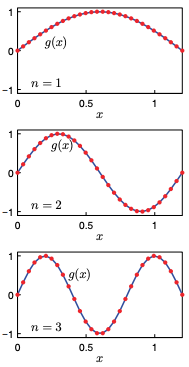
\includegraphics[width=\marginparwidth]{fig34}\captionof{figure}{The first three eigenfunctions found in 3.3. The points are the numerical eigenfunctions and the line is the exact solution.}}

	\begin{enumerate}[label=(\alph*)]
	\item  Write a program to numerically find the eigenvalues and eigenvectors
of Eq. \eqref{eg:35} using the procedure outlined above. Use $N = 30, \mu = 0.003,
T = 127,$ and $L = 1.2$. Write a loop that plots each of the eigenvectors.
You will find two infinite eigenvalues together with odd-looking eigenvectors that don\rq t satisfy the boundary conditions. These two show up
because of the two rows of the B matrix that are filled with zeros. They
are numerical artifacts with no physical meaning, so just ignore them.
The eigenvectors of the higher modes start looking jagged. These
must also be ignored because they are poor approximations to the
continuous differential equation in Eq. \eqref{eg:35}.
	\item A few of the smooth eigenfunctions are very good approximations.
Plot the eigenfunctions corresponding to $n = 1,2,3$ and compare them
with the exact solutions in Eq. \eqref{eg:38}. Since the modes include an
arbitrary scaling $g_0$, you won\rq t find the amplitudes match unless you
choose an appropriate value for $g_0$. Calculate the exact values for $\lambda$
using Eq. \eqref{eg:39} and compare them with the numerical eigenvalues.
Now compare your numerical eigenvalues for the $n = 20$ mode with
the exact solution. What is the trend in the accuracy of the eigenvalue
method?
	\item The first few values for $\lambda$ should match the resonances that you found
in 3.2(b). Go back to your calculation in 3.2(b) and make two plots
of the steady state amplitude for driving frequencies near these two
resonant values of $\lambda$. For each plot, choose a small range of frequencies that brackets the resonance frequency above and below. You
should find very large amplitudes, indicating that you are right on the
resonances.
	\end{enumerate}
	Finally let\rq s explore what happens to the eigenmode shapes when we change
the boundary conditions.

\paragraph*{P3.4}
	\marginpar{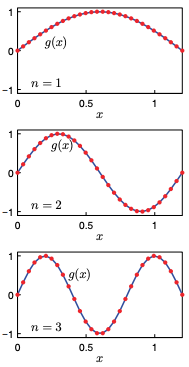
\includegraphics[width=\marginparwidth]{fig34}\captionof{figure}{The first three eigenfunctions for $3.4$ (a).}}
\begin{enumerate}[label=(\alph*)]
	\item Change your program from problem 3.3 to implement the boundary
condition  \begin{equation*}
		g^\prime(L) = 0
				\end{equation*}
				This boundary condition describes what happens if one end of the
string is free to slide up and down rather than attached to a fixed
position. Use the approximation you derived in problem 2.4(b) for the
derivative $g^\prime(L)$ to implement this boundary condition, i.e
\begin{equation*}
		g^\prime(L) \approx \frac{1}{2h}g_{N-3} - \frac{2}{h}g_{N-2} + \frac{3}{2h}g_{N-1}
				\end{equation*}Explain physically why the resonant frequencies change as they do.
				\item In some problems mixed boundary conditions are encountered, for
example\begin{equation*}
		g^\prime(L) = 2g(L)
				\end{equation*}Find the first few resonant frequencies and eigenfunctions for this
case. Look at your eigenfunctions and verify that the boundary condition is satisfied. Also notice that one of your eigenvalues corresponds
to $\omega^2$ being negative. This means that the nice smooth eigenfunction
associated with this eigenvalue is not physical in our wave resonance
problem with this boundary condition. The code snippet we gave you
above will have trouble with the np.sqrt. You can just look at the
values of $\omega^2$ instead
\end{enumerate}
\chapter*{The Hanging Chain and Quantum Bound States}
\addcontentsline{toc}{chapter}{The Hanging Chain and Quantum Bound States} 
\section*{Resonance for a hanging chain}
\addcontentsline{toc}{section}{Resonance for a hanging chain} 
	\marginpar{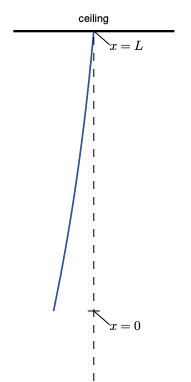
\includegraphics[width=\marginparwidth]{fig41}\captionof{figure}{The first normal mode for a hanging chain.}}

In the last lab, we studied waves on a string with constant tension and observed
sinusoidal normal modes of vibration. We\rq ll start off this lab by studying the
problem of standing waves on a hanging chain. It was the famous Swiss mathematician Johann Bernoulli who discovered in the 1700s that a draped hanging
chain has the shape of a \lq\lq catenary\rq\rq, or the hyperbolic cosine function. The problem of the normal mode frequencies of a vertical hanging chain was solved by
Johann\rq s son, Daniel Bernoulli, and is the first time that the function that later
became known as the $J_0$ Bessel function showed up in physics.
For a hanging chain, the tension varies with position—the tension at the top
is large (since it supports the weight of the whole chain) and the tension at the
bottom is essentially zero.1 We are going to find its normal modes of vibration of a
hanging chain using the method of Problem 3.3. The wave equation for transverse
waves on a chain with varying tension $T (x)$ and constant linear mass density $\mu$ is
given $by^2$

\begin{equation}\label{eq:41}
		\mu \frac{\partial^2 y}{\partial t^2} - \frac{\partial}{\partial x}(T(x)\frac{\partial y}{\partial x}) = 0
				\end{equation}
				
		We\rq ll use a coordinate system that defines $x = 0$ as the bottom of the chain and
$x = L$ as the ceiling.		

\paragraph*{P4.1}
Use the fact that a stationary hanging chain is in equilibrium to draw a
free-body diagram for a link at an arbitrary $x$. Use this diagram to show that
the tension in the chain as a function of $x$ is given by
	\begin{equation}\label{eq:42}
		T(x) = \mu g x
				\end{equation}		
				where $\mu$ is the linear mass density of the chain and $g = 9.8 m/s^2$
is the acceleration of gravity. Then show that Eq. \eqref{eg:41} reduces to	
	\begin{equation}\label{eq:43}
		 \frac{\partial^2 y}{\partial t^2} - g\frac{\partial}{\partial x}(x\frac{\partial y}{\partial x}) = 0
				\end{equation}	
				for a freely hanging chain.
			As in Lab 3, we now look for normal modes by separating the variables:
$y(x,t) = f(x)\cos(\omega t)$. We then substitute this form for $y(x,t)$ into \eqref{eg:43} and simplify to obtain	
		\begin{equation}\label{eq:44}
		 x \frac{d^2 f}{dx^2}+\frac{df}{dx} = - \frac{\omega^2}{g}f
				\end{equation}		
				which is in eigenvalue form with $ \lambda = −\omega^2/g$ . The boundary condition at the
ceiling is $f (L) = 0$ while the boundary condition at the bottom is obtained by
taking the limit of Eq. \eqref{eg:44} as $x \rightarrow 0$ to find
	\begin{equation}\label{eq:45}
		f^\prime(x) = - \frac{\omega^2}{g}f(0) = \lambda f(0)
				\end{equation}		
			\marginpar{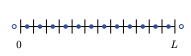
\includegraphics[width=\marginparwidth]{fig42}\captionof{figure}{A cell-centered grid with ghost points. (The open circles are the ghost points.)}}		
				In the past couple labs we dealt with derivative boundary conditions by fitting
a parabola to the last three points on the grid and then taking the derivative of
the parabola (e.g. Problems 2.4(b) and 3.4). This time we\rq ll handle the derivative
boundary condition by using a cell-centered grid with ghost points, as discussed
in Lab 1. Recall that a cell-center grid divides the spatial region from 0 to L into
N cells with a grid point at the center of each cell. We then add two more grid
points outside of $[0,L]$, one at $x_0  = −h/2$ and the other at $x_{N+1} = L + h/2$. The
ghost points are used to apply the boundary conditions. By defining N as the
number of interior grid points (or cells), we have $N +2$ total grid points, which
may seem weird to you. We prefer it, however, because it reminds us that we are
using a cell-centered grid with N physical grid points and two ghost points. \\
With this grid there isn\rq t a grid point at each endpoint, but rather we have two
grid points that straddle each endpoint. If the boundary condition specifies a
value, like $f (L) = 0 $ in the problem at hand, we use a simple average like this:
	\marginpar{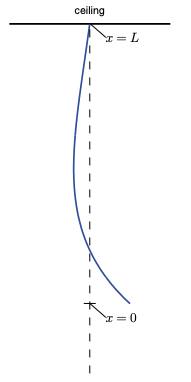
\includegraphics[width=\marginparwidth]{fig43}\captionof{figure}{The shape of the second mode of a hanging chain}}
\begin{equation}\label{eq:46}
		\frac{f_{N+1} + f_N}{2}=0
				\end{equation}	

For $f^\prime (L) = 0$, a centered derivative around $x = L$ yields
\begin{equation}\label{eq:47}
		\frac{f_{N+1} + f_N}{h}=0
				\end{equation}	
				\paragraph*{P4.2}
				\begin{enumerate}[label=(\alph*)]
			\item	On paper, write out the discretized version of Eq. \eqref{eg:44} and put it in
the form of a generalized eigenvalue problem
\begin{equation}\label{eq:48}
		Af = \lambda B f
				\end{equation}
					Remember that for the interior points, the matrix B is just the identity
matrix with 1 on the main diagonal and zeros everywhere else. Decide on the values needed in the bottom rows of A and B to give the
boundary condition in Eq. \eqref{eg:46} at $x = L$ (the ceiling) no matter what
$\lambda$ turns out to be.
	\marginpar{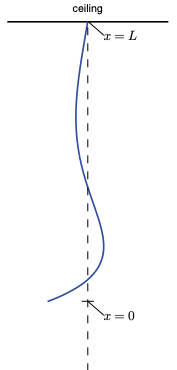
\includegraphics[width=\marginparwidth]{fig44}\captionof{figure}{The shape of the third mode of a hanging chain}}
\item Now let\rq s decide how to handle the derivative boundary condition at
$x = 0$ (the bottom of the chain), given by Eq. \eqref{eg:45}. Since this condition
is already in eigenvalue form we don\rq t load the top row of B with zeros.
Instead we load A with the left operator $f^\prime (0)$ according to Eq. \eqref{eg:47}
and B with the right operator $f(0)$  according to Eq. \eqref{eg:46}. Leave the
eigenvalue $ \lambda = − \omega ^ 2
/g$ out of the top row of B since the matrix equation
$Af = \lambda Bf$ already has the λ multiplying B. Write down the values
needed in the top rows of A and B, perform the matrix multiplication
for this row, and verify that your choices correctly produce Eq. \eqref{eg:45}.
\item Write a program to load the matrices A and B with $L = 2 m$ (or the measured length if different). Then solve for the normal modes of vibration
of a hanging chain. As in Lab 3, some of the eigenvectors are not physical because they don’t satisfy the boundary conditions; ignore them.
Compare your numerical resonance frequencies to measurements
made on the chain hanging from the ceiling in the classroom
\item The analytic solution to Eq. \eqref{eg:44} without any boundary conditions is
\begin{equation*}
		f(x) = c_1J_0(2\omega \sqrt{x / g}) + c_2 Y_0(2\omega \sqrt{2\omega \sqrt{x / g}})
				\end{equation*}
				where $J_0$ and $Y_0$ are the Bessel functions of the first and second kind,
respectively. The boundary condition at $x = 0$ rules out $Y_0$, since it is
singular at $x = 0$. Apply the condition $f(L) = 0$ to find analytically the
mode frequencies $ \omega_i$
in terms of the values xi that satisfy $J_0(xi) = 0$.
Verify that these values agree with the ω values from part (c).
HINT: The $scipy.special$ library has a function $jn_zeros(n,i)$
that will return the first $i$ values of $x$ for which $J_n(x)$ is zero.
				\end{enumerate}
				

\section*{Quantum bound states}
\addcontentsline{toc}{section}{Quantum bound states} 
Now let\rq s jump forward several centuries in physics history and study bound
quantum states using the same techniques we used to study the modes of a
hanging chain. Schrödinger\rq s equation for a potential well $V(x)$ is

\begin{equation}\label{eq:49}	
i \bar{h} \frac{\partial \Psi}{\partial t} = - \frac{\bar{h}^{2}}{2 m} \frac{\partial^{2} \Psi}{\partial x^{2}}+V(x) \Psi
				\end{equation}
				
		If we assume a separable solution of the form $\Psi(x,t) = \Psi(x)e^{
−i Et/ħ}$
and plug this
into Eq. \eqref{eg:49}, we find the time-independent Schrödinger equation

\begin{equation}\label{eq:410}
-\frac{\bar{h}^{2}}{2 m} \frac{d^{2} \psi}{d x^{2}}+V(x) \psi=E \psi
\end{equation}
For a particle in a one-dimensional harmonic oscillator, with $V (x) = kx^2/2$, this
becomes
\begin{equation}\label{eq:411}
-\frac{\bar{h}^{2}}{2 m} \frac{d^{2} \psi}{d x^{2}}+\frac{1}{2} k x^{2} \psi=E \psi
\end{equation}
with boundary conditions $\psi = 0$ at ±∞. Note that k is not the wave number; it is
the spring constant, $F = −kx$, with units of Newtons/meter.
The numbers that go into Schrödinger’s equation are so small that it makes
it difficult to tell what size of grid to use. For instance, using lengths like 2, 5, or
10 meters would be completely ridiculous for the bound states of an atom where
the typical size is on the order of $10^{−10}$ m. Some physicists just set $ħ, m$, and $k$
to unity, but this is bad practice. If you do this, you won\rq t know what physical
parameters your numerical results describe. The correct procedure is to \lq\lq rescale \rq\rq
the problem. \\ 
The goal of rescaling is to replace physical variables like x with unitless variables like $\xi = x/a$, where a is a \lq\lq characteristic \rq\rq length written in terms of the other
variables in the problem. Since a is a length, $\xi$ is unitless, and since a is scaled
to the problem parameters, $\xi$ will typically have magnitudes around the size of 1.
Let\rq s practice this procedure for the problem at hand.
	\marginpar{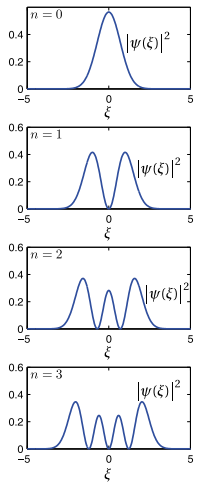
\includegraphics[width=\marginparwidth]{fig45}\captionof{figure}{The probability distributions for the ground state and the first three excited states of the harmonic oscillator.}}
\paragraph*{P4.3}  Substitute $x = \alpha \xi$ into Eq. \eqref{eg:411}, and then do some algebra to put the
equation in the form
\begin{equation}\label{eq:412}
-\frac{C}{2} \frac{d^{2} \psi}{d \xi^{2}}+\frac{1}{2} \xi^{2} \psi=\frac{E}{\bar{E}} \psi
\end{equation}
where the constants $C$ and $\bar{E}$ involve factors like $ħ, m, k$, and $a$.
Now make the differential operator on the left be as simple as possible by
choosing to make $C = 1$. This determines how the characteristic length a
depends on $ħ, m$, and $k$. Once you have determined a in this way, check to
see that it has units of length. You should find

\begin{equation}\label{eq:413}
a=\left(\frac{\bar{h}^{2}}{k m}\right)^{1 / 4}=\sqrt{\frac{\bar{h}}{m \omega}}, \quad \text { where } \quad \omega=\sqrt{\frac{k}{m}}
\end{equation}
Finally, rescale the energy by writing introducing a new variable $	\epsilon = E/\bar{E}$.
Show that $\bar{E}$ has units of energy, so that ϵ is unitless. You should find that
 \begin{equation}\label{eq:414}
\bar{E} = \bar{h}\sqrt{\frac{k}{m}}
\end{equation}
The final scaled version of Schrödinger\rq s equation then becomes
\begin{equation}\label{eq:415}
-\frac{1}{2} \frac{d^{2} \psi}{d \xi^{2}}+\frac{1}{2} \xi^{2} \psi=\epsilon \psi
\end{equation}
When you solve this equation and find results in terms of $\epsilon$ and $\xi$, you can
use the equations above to translate them into real-world values of E and x.\\
Now that Schrödinger\rq s equation is in dimensionless form, we are ready to
solve it with out standard technique.


\paragraph*{P4.4}
	\marginpar{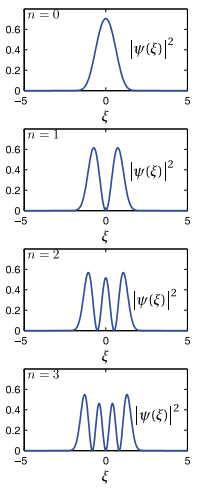
\includegraphics[width=\marginparwidth]{fig46}\captionof{figure}{The probability distributions for the ground state and the first three excited states for the potential in Problem 4.5}}
Discretize Eq. \eqref{eq:415} on paper. Then write a program to do this eigenvalue
problem, similar to the other programs we\rq ve written recently. The boundary conditions are that both the value and derivative of $\psi$ should go to zero
at $\xi$ = $\infty +$. Since you\rq ve scaled the problem, it makes sense to choose a
cell-edge grid that goes from $\xi =  - 5$ to $\xi  = 5$, or some other similar pair
of numbers. These numbers are supposed to approximate infinity in this
problem. Just set the value of $\psi$ to zero at the edge-points and make sure
(by looking at the eigenfunction solutions) that your grid is large enough
that the wave function has zero slope at the edges of the grid.


\begin{enumerate}[label=(\alph*)]
\item Plot the first several bound states. As a guide, Figure 4.5 displays the square
of the wave function for the first few excited states. (The amplitude has
been appropriately normalized so that $ \int |ψ(x)|^2 = 1$
\item  If you look in a quantum mechanics textbook you will find that the bound
state energies for the simple harmonic oscillator are given by the formula
\begin{equation}\label{eq:416}
E_n = (n + \frac{1}{2}) \bar{h}\sqrt{\frac{k}{m}} =(b+\frac{1}{2})\bar{E}
\end{equation}
so that the dimensionless energy eigenvalues $\epsilon_n$ are given by
\begin{equation}\label{eq:417}
\epsilon_n = n + \frac{1}{2}
\end{equation}
Verify that this formula for the bound state energies is correct for $n =
0,1,2,3,4$
\paragraph*{P4.5}
Now redo this entire problem, but with the harmonic oscillator potential
replaced by
\begin{equation}\label{eq:418}
V(x)=\mu x^4
\end{equation}
so that we have

\begin{equation}\label{eq:419}
-\frac{\bar{h}^{2}}{2 m} \frac{d^{2} \psi}{d x^{2}}+\mu x^{4} \psi=E \psi
\end{equation}
With this new potential you will need to find new formulas for the characteristic length and energy so that you can use dimensionless scaled variables as
you did with the harmonic oscillator. Choose a so that your scaled equation
is
\begin{equation}\label{eq:420}
- \frac{1}{2} \frac{d^{2} \psi}{d \xi^{2}} + \xi^{4} \psi = \epsilon \psi
\end{equation}

with $E = \epsilon \bar{3}$ . Use algebra by hand to show that

\begin{equation}\label{eq:421}
a=\left(\frac{\bar{h}^{2}}{m \mu}\right)^{1 / 6} \quad \bar{E}=\left(\frac{\bar{h}^{4} \mu}{m^{2}}\right)^{1 / 3}
\end{equation}
Find the first 5 bound state energies by finding the first 5 values of $ \epsilon_n $ in the
formula $E_n =  \epsilon_n \bar{E}$.

\end{enumerate}
\chapter*{Animating the Wave Equation: Staggered Leapfrog}
\addcontentsline{toc}{chapter}{Animating the Wave Equation: Staggered Leapfrog} 
In the last couple of labs we handled the wave equation by Fourier analysis,
turning the partial differential equation into a set of ordinary differential equations using separation of variables.1 But separating the variables and expanding
in orthogonal functions is not the only way to solve partial differential equations,
and in fact in many situations this technique is awkward, ineffective, or both. In
this lab we will study another way of solving partial differential equations using a
spatial grid and stepping forward in time. As an added attraction, this method
automatically supplies a beautiful animation of the solution. There are several
algorithms of this type that can be used on wave equations, so this is just an
introduction to a larger subject. The method we will show you here is called
staggered leapfrog; it is the simplest good method that we know


\section*{The wave equation with staggered leapfrog}
\addcontentsline{toc}{section}{The wave equation with staggered leapfrog} 
Consider again the classical wave equation with wave speed c.

\begin{equation}\label{eq:51}
	\frac{\partial^2 y}{\partial t^2} - c^2 \frac{\partial^2 y}{\partial x^2} = 0
\end{equation}
For a string, the wave speed is related to tension and density via $c = \sqrt{T / \mu} $ The
boundary conditions are usually either of Dirichlet type (values specified):
\begin{equation}\label{eq:52}
	y(0,t) = f_{left}(t) ; y(L,t) = f_{right}(t)
\end{equation}
or of Neumann type (derivatives specified):
\begin{equation}\label{eq:53}
	\frac{\partial y}{\partial x} (0)  = g_{left}(t) ; \frac{\partial y}{\partial x} (L)  = g_{right}(t)
\end{equation}
Sometimes mixed boundary conditions specify a relation between the value
and derivative, as at the bottom of the hanging chain. In any case, some set of
conditions at the endpoints are required to solve the wave equation. It is also
necessary to specify the initial state of the string, giving its starting position and
velocity as a function of position:
\begin{equation}\label{eq:54}
	y(x,t = 0) = y_0(x) \quad ; \quad \frac{\partial y(x,t)}{\partial t} \vert_{t=0} = v_0 (x)
\end{equation}
Both of these initial conditions are necessary because the wave equation is second
order in time, just like Newton\rq s second law, so initial displacement and velocity
must be specified at each point to find a unique solution.
To numerically solve the classical wave equation via staggered leapfrog we
approximate both the temporal and spatial derivatives in Eq.\eqref{eg:51} with centered
finite differences, like this:
\begin{equation}\label{eq:55}
\begin{aligned}
&\frac{\partial^{2} y}{\partial t^{2}} \approx \frac{y_{j}^{n+1}-2 y_{j}^{n}+y_{j}^{n-1}}{\tau^{2}} \\
&\frac{\partial^{2} y}{\partial x^{2}} \approx \frac{y_{j+1}^{n}-2 y_{j}^{n}+y_{j-1}^{n}}{h^{2}}
\end{aligned}
\end{equation}
In this notation, spatial position is indicated by a subscript $j$, referring to grid
points $x_j$, while position in time is indicated by superscripts $n$, referring to time
points $t_n$ so that $y(x_j,t_n) = y_j^n$. The time steps and the grid spacings are assumed to be uniform with time step called
$\tau$ and grid spacing called $h$. The staggered leapfrog algorithm aims to find $y_j$ one time step into the future, denoted by $y_j^{n+1}$,
from the current and previous values of $y_j$. To derive the algorithm put Eqs.\eqref{eg:55} into Eq. \eqref{eg:51} and solve for $y_j^{n+1}$ to find
\begin{equation}\label{eq:56}
	y_j^{n+1} = 2y_j^n - y_j^{n-1} + \frac{c^2 \tau^2}{h^2}(y_{j+1}^n - 2y^n_j + y^n_{j-1})
\end{equation}

\paragraph*{P5.1} Derive Eq. \eqref{eg:56} using the approximate second derivative formulas. This is
really simple, so just do it on paper.
Equation \eqref{eg:56} can only be used at interior spatial grid points because the
$ j + 1 {or} j-1$  indices reach beyond the grid at the first and last grid points. The
behavior of the solution at these two end points is determined by the boundary
conditions. Since we will want to use both fixed value and derivative boundary
conditions, let\rq s use a cell-centered grid with ghost points (with $N$ cells and $N+2$ grid points) so we can easily handle both types without changing our grid. If the values at the ends are specified we have 
\begin{equation}\label{eq:57}
\begin{gathered}
\frac{y_{0}^{n+1}+y_{1}^{n+1}}{2}=f_{\text {left }}\left(t_{n+1}\right) \Rightarrow y_{0}^{n+1}=-y_{1}^{n+1}+2 f_{\text {left }}\left(t_{n+1}\right) \\
\frac{y_{N+1}^{n+1}+y_{N}^{n+1}}{2}=f_{\text {right }}\left(t_{n+1}\right) \Rightarrow y_{N+1}^{n+1}=-y_{N}^{n+1}+2 f_{\text {right }}\left(t_{n+1}\right)
\end{gathered}
\end{equation}
If the derivatives are specified then we have
\begin{equation}\label{eq:58}
\begin{aligned}
&\frac{y_{1}^{n+1}-y_{0}^{n+1}}{h}=g_{\text {left }}\left(t_{n+1}\right) \Rightarrow y_{0}^{n+1}=y_{1}^{n+1}-h g_{\text {left }}\left(t_{n+1}\right) \\
&\frac{y_{N+1}^{n+1}-y_{N}^{n+1}}{h}=g_{\text {right }}\left(t_{n+1}\right) \Rightarrow y_{N+1}^{n+1}=y_{N}^{n+1}+h g_{\text {right }}\left(t_{n+1}\right)
\end{aligned}
\end{equation}
To use staggered leapfrog, we first advance the solution at all interior points to
the next time step using Eq. \eqref{eg:56}, then we apply the boundary conditions using
the appropriate equation from Eqs. \eqref{eg:57}-\eqref{eg:58} to find the values of y at the end
points, and then we are ready to take another time step.
The staggered leapfrog algorithm in Eq. \eqref{eg:56} requires not just y at the current
time level $ y_j^n$ but also $y$ at the previous time level $y^{n−1}_j$. This means that we\rq ll need
to keep track of three arrays: an array y for the current values $ y_j^n$, an array yold
for the values at the previous time step $ y_j^{n-1}$, and an array ynew for the values
at the next time step $ y_j^{n+1}$. At time $t = 0$ when the calculation starts, the initial
position condition gives us the current values $ y_j^n$ , but we\rq ll have to make creative
use of the initial velocity condition to create an appropriate yold to get started.
To see how this works, let\rq s denote the initial values of y on the grid by $ y_j^0 $, the
values after the first time step by $ y_j^{1} $, and the unknown previous values (yold) by
$ y_j^{-1} $. A centered time derivative at $t = 0$ turns the initial velocity condition from
Eq. \eqref{eg:54} into
\begin{equation}\label{eq:59}
\frac{y_j^1 - y_j^{-1}}{2 \tau} = v_0(x_j)
\end{equation}
This gives us an equation for the previous values $y_j^{-1}$ , but it is in terms of the
still unknown future values $y_j^{1}$. However, we can use Eq. (5.6) to obtain another
relation between $y_j^{1}$and $y_j^{-1}$. Leapfrog at the first step ($n = 0$) says that
\begin{equation}\label{eq:510}
y_j^1 = 2Y^0_j - y_j^{-1} + \frac{c^2 \tau^2}{h^2}(y^0_{j+1}-2y^0_j+y^0_{j-1})
\end{equation}
If we insert this expression for $y^1_j$ into Eq. \eqref{eg:59}, we can solve for $y^{-1}_j $ in terms of
known quantities:
\begin{equation}\label{eq:511}
y_j^{-1} = Y^0_j - v_0(x_j)\tau + \frac{c^2 \tau^2}{2h^2}(y^0_{j+1}-2y^0_j+y^0_{j-1})
\end{equation}

\paragraph*{P5.2}Derive Eq. \eqref{eq:511} from Eqs. \eqref{eq:59} and \eqref{eq:510}. Again, just use paper and pencil.
OK; we are now ready to code the staggered leapfrog algorithm.
\paragraph*{P5.3}

\begin{enumerate}[label=(\alph*)]
\item Start by making a cell-centered $x$ grid with ghost points over the region
$0 \leq x \leq L$, with $L = 1$ m. Use $N = 200$ cells, so you have 202 grid
points. Define the initial displacement $y$ as Gaussian bump with 1 cm
amplitude in the middle of the string, like this
\begin{lstlisting}
y = 0.01 * np.exp(-(x-L/2)**2 / 0.02)
\end{lstlisting}
and the initial velocity $vy$ to be zero everywhere along the string. Used
fixed-value boundary conditions, with $y(0) = 0$ and $y(L) = 0$. Plot the
initial position just to make sure your grid is right and that your initial
position array looks reasonable
\item Assume that the wave speed on this string is $c = 2$ m/s, and pick
the time step as $tau = 0.2*h/c$. (We\rq ll explore this choice more
later.) Then create a variable yold using Eq. \eqref{eg:511}, and enforce the boundary conditions on yold. As you write this code, don\rq t write a
bunch of for loops to iterate through all the points. Instead, assign all
interior points at once using the NumPy array colon indexing method
(e.g. $y[1:-1]$ accesses all the interior points of $y$) and then set the
boundary conditions explicitly
\item Now it is time to code the main staggered leapfrog algorithm and make
an animation of the solution. Since it has been a couple of labs since
we made an animation, here is a framework for the code to remind
you of the basic animation commands:
	\marginpar{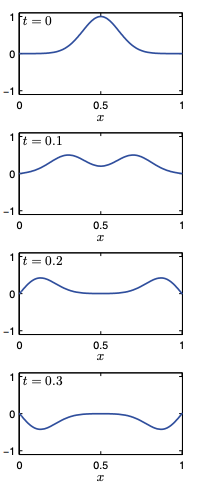
\includegraphics[width=\marginparwidth]{fig51}\captionof{figure}{Snapshots of the evolution of a wave on a string with fixed ends and an initial displacement but no initial velocity. (See Problem 5.3(b))}}
\begin{lstlisting}
ynew = np.zeros_like(y)
j = 0
t = 0
tmax = 2
plt.figure(1) # Open the figure window
# the loop that steps the solution along
while t < tmax:
j = j+1
t = t + tau
# Use leapfrog and the boundary conditions
# to load ynew with y at the next time
# step using y and yold
# update yold and y for next timestep
# remember to use np.copy
# make plots every 50 time steps
if j % 50 == 0:
plt.clf() # clear the figure window
plt.plot(x,y,'b-')
plt.xlabel('x')
plt.ylabel('y')
plt.title('time={:1.3f}'.format(t))
plt.ylim([-0.03,0.03])
plt.xlim([0,1])
plt.draw() # Draw the plot
plt.pause(0.1) # Give the computer time to draw
\end{lstlisting}
The actual staggered leapfrog code is missing above. You’ll need to
write that. Run the animations long enough that you can see the
reflection from the ends and the way the two pulses add together and
pass right through each other.
\item Once you have it running, experiment with various time steps $\tau$. Show
by numerical experimentation that if$ \tau > h/c$ the algorithm blows up
spectacularly. This failure is called a numerical instability and we
will be trying to avoid it all semester. This limit is called the CourantFriedrichs-Lewy condition, or sometimes the CFL condition, or 

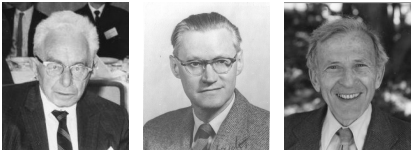
\includegraphics[width=\marginparwidth]{fig52}\captionof{figure}{Richard Courant (left), Kurt Friedrichs (center), and Hans Lewy (right) described the CFL instability condition in 1928 .}


sometimes (unfairly) just the Courant condition
	\marginpar{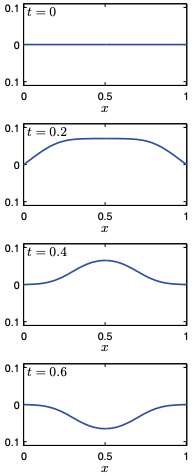
\includegraphics[width=\marginparwidth]{fig53}\captionof{figure}{ Snapshots of the evolution of a wave on a string with fixed ends and no initial displacement but with an initial velocity. (See Problem 5.3(f))}}
\item Change the boundary conditions so that $ \frac{\partial y}{\partial x} = 0 $ at each end and watch
how the reflection occurs in this case.
\item Change the initial conditions from initial displacement with zero
velocity to initial velocity with zero displacement. Use an initial Gaussian velocity pulse just like the displacement pulse you used earlier
and use fixed-end boundary conditions. Watch how the wave motion
develops in this case. (You will need to change the y-limits in the axis
command to see the vibrations with these parameters.) Then find a
slinky, stretch it out, and whack it in the middle to verify that the math
does the physics right.

\end{enumerate}

\section*{The damped wave equation}
\addcontentsline{toc}{section}{The damped wave equation} 
We can modify the wave equation to include damping of the waves using a linear
damping term, like this:
\begin{equation}\label{eq:512}
\frac{\partial^2 y}{\partial t^2} + \Upsilon \frac{\partial y}{\partial t} - c^2 \frac{\partial^2 y}{\partial x^2} = 0
\end{equation}
with $c$ constant. The staggered leapfrog method can be used to solve Eq. \eqref{eg:512}
also. To do this, we use the approximate first derivative formula
\begin{equation}\label{eq:513}
\frac{\partial y}{\partial t } \approx = \frac{y_j^{n+1} - y_j^{n-1}}{2 \tau}
\end{equation}
along with the second derivative formulas in Eqs. \eqref{eg:55} and find an expression for
the values one step in the future:
\begin{equation}\label{eq:514}
y^{n+1}_j = \frac{1}{2+ \Upsilon \tau}(4y^n_j-2y^{n-1}_j+ \Upsilon \tau y^{n-1}_j + \frac{2c^2 \tau^2}{h^2}(y^n_{j+1} - 2y^n_j + y^n_{j-1}))
\end{equation}
\paragraph*{P5.4} 
\begin{enumerate}[label=(\alph*)]
	\item Derive Eq. \eqref{eg:514}.
	\item Find a new formula for the initial value of yold using Eqs.\eqref{eg:59} and
\eqref{eg:514}. When you get the answer, ask your TA or instructor to check to
see if you got it right.
\item Modify your staggered leapfrog code to include damping with $ \Upsilon = 0.2$.
Then run your animation with the initial conditions in Problem 5.3(c)
and verify that the waves damp away. You will need to run for about
25 s and you will want to use a big skip factor so that you don\rq t have
to wait forever for the run to finish. Include some code to record the
maximum value of $y(x)$ over the entire grid as a function of time and
then plot it as a function of time at the end of the run so that you can
see the decay caused by $\Upsilon$. The decay of a simple harmonic oscillator
is exponential, with amplitude proportional to $e^{−\Upsilon^{ t/2}}$. Scale this time
decay function properly and lay it over your maximum y plot to see if
it fits. Can you explain why the fit is as good as it is? (Hint: think about
doing this problem via separation of variables.)

\end{enumerate}
	\marginpar{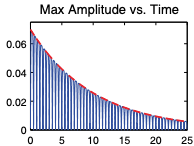
\includegraphics[width=\marginparwidth]{fig54}\captionof{figure}{The maximum amplitude of oscillation decays exponentially for the damped wave equation. (Problem $5.4(\mathrm{c})$ )}}
\section*{The damped and driven wave equation}
\addcontentsline{toc}{section}{The damped and driven wave equation} 
Finally, let\rq s look at what happens when we add an oscillating driving force to our
string, so that the wave equation becomes
\begin{equation}\label{eq:515}
\frac{\partial^2 y}{\partial t^2} + \Upsilon \frac{\partial y}{\partial t}-c^2\frac{\partial^2 y}{\partial x^2} = \frac{f(x)}{\mu} \cos(\omega t )
\end{equation}

At the beginning of Lab 3 we discussed the qualitative behavior of this system.
Recall that if we have a string initially at rest and then we start to push and pull on
a string with an oscillating force/length of $f(x)$, we launch waves down the string.
These waves reflect back and forth on the string as the driving force continues
to launch more waves. The string motion is messy at first, but the damping in
the system causes the the transient waves from the initial launch and subsequent
reflections to eventually die away. In the end, we are left with a steady-state
oscillation of the string at the driving frequency $\omega$.
Now that we have the computational tools to model the time evolution of the
system, let\rq s watch this behavior.
\paragraph*{P5.5}

\begin{enumerate}[label=(\alph*)]
\item Re-derive the staggered leapfrog algorithm to include both driving
and damping forces as in Eq. \eqref{eg:515}.
\item Modify your code from Problem 5.4 to use this new algorithm. We\rq ll
have the string start from rest, so you don\rq t need to worry about finding
yold. Just set $y = 0$ and $yold = 0$ and enter the time-stepping loop.
This problem involves the physics of waves on a real guitar string,
so we\rq ll need to use realistic values for our parameters. Use $T = 127$,
$ \mu = 0.003$, and$ L = 1.2$ (in SI units) and remember that $ c = \sqrt{T / \mu}$. Use the same driving force as in Problem 3.2(a)

\begin{equation}\label{eq:516}
f(x)= \begin{cases}0.73 & \text { if } 0.8 \leq x \leq 1 \\ 0 & \text { otherwise }\end{cases}
\end{equation}
and set the driving frequency at $\omega = 400$. Choose a damping constant
$\Upsilon$ that is the proper size to make the system settle down to steady state
after 20 or 30 bounces of the string. (You will have to think about the
value of  $\omega$ that you are using and about your damping rate result from
problem 5.4 to decide which value of $\Upsilon$ to use to make this happen.)
Run the model long enough that you can see the transients die away
and the string settle into the steady oscillation at the driving frequency.
You may find yourself looking at a flat-line plot with no oscillation at
all. If this happens look at the vertical scale of your plot and remember
that we are doing real physics here. If your vertical scale goes from −1
to 1, you are expecting an oscillation amplitude of 1 meter on your
guitar string. Compare the steady state mode to the shape found in
Problem 3.2(a) (see Fig. 3.1).
Then run again with $ \omega = 1080 $, which is close to a resonance, and again
see the system come into steady oscillation at the driving frequency.
\end{enumerate}
	\marginpar{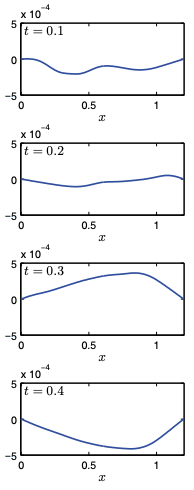
\includegraphics[width=\marginparwidth]{fig55 }\captionof{figure}{Snapshots of the evolution a driven and damped wave with $\omega=400$. As the transient behavior dies out, the oscillation goes to the resonant mode. To make the pictures more interesting, the string was not started from rest in these plots. (In Problem $5.5$ you start from rest for easier coding.]}}

\chapter*{The 2-D Wave Equation With Staggered Leapfrog}
\addcontentsline{toc}{chapter}{The 2-D Wave Equation With Staggered Leapfrog} 
\section*{Two dimensional grids}
\addcontentsline{toc}{section}{Two dimensional grids} 

	\marginpar{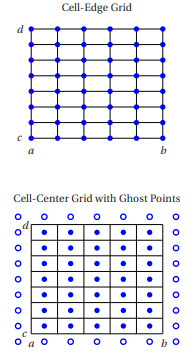
\includegraphics[width=\marginparwidth]{fig61}\captionof{figure}{Two types of 2-D grids.}}
In this lab we will do problems in two spatial dimensions, $x$ and $y$, so we need
to spend a little time thinking about how to represent 2-D grids. For a simple
rectangular grid where all of the cells are the same size, 2-D grids are pretty
straightforward. We just divide the $x$-dimension into equally sized regions and
the $y$-dimension into equally sized regions, and the two one dimensional grids
intersect to create rectangular cells. Then we put grid points either at the corners
of the cells (cell-edge) or at the centers of the cells (cell-centered). On a cell-center
grid we\rq ll usually want ghost point outside the region of interest so we can get the
boundary conditions right. \\ NumPy has a nice way of creating rectangular two-dimensional grids using
the meshgrid command. You can create 2-d rectangle defined by $x \in [a,b]$ and
$y \in [c,d]$ and then plot a function on that grid this way:
\begin{lstlisting}
from mpl_toolkits.mplot3d import Axes3D
import matplotlib.pyplot as plt
from matplotlib import cm
import numpy as np
# Make 1D x and y arrays
Nx=20
a=-1.5
b=1.5
x,hx = np.linspace(a,b,Nx,retstep = True)
Ny=10
c=-1.2
d=1.2
y,hy = np.linspace(c,d,Ny,retstep = True)
# Make the 2D grid and evaluate a function
X, Y = np.meshgrid(x,y,indexing='ij')
Z = X**2 + Y**2
# Plot the function as a surface.
fig = plt.figure(1)
ax = fig.gca(projection='3d')
surf = ax.plot_surface(X, Y, Z, cmap=cm.viridis)
plt.xlabel('x')
plt.ylabel('y')
fig.colorbar(surf)
\end{lstlisting}
The argument $indexing='ij'$ in the meshgrid function switches the ordering
of the elements in the resulting matrices from the matrix indexing convention
$Z[row,col]$ to the function indexing convention $Z[x_i,y_y]$ for representing $Z(x_i, y_i)$.

\paragraph*{P6.1} 

\begin{enumerate}[label=(\alph*)]
\item
Use the code fragment above in a program to create a 30-point celledge grid in $x$ and a 50-point cell-edge grid in $y$ with $a = 0, b = 2,
c = −1, d = 3$. Switch back and forth between $indexing='ij'$ and
$indexing='xy'$, and look at the different matrices that result. Convince the TA that you know what the difference is. (HINT: When
we write matrices, rows vary in the $y$ dimension and columns vary
in the $x$ direction, whereas with $Z(x_i, y_i)$ we have a different convention. NumPy\rq s naming convention seems backward to us, but
we didn\rq t come up with it. Sorry.) We recommend that you use the
$indexing='ij'$ convention, as it tends to more readable code for representing $Z(x_i, y_i)$.
\item  Using this 2 - D grid, evaluate the following function of $x$ and $y$:
\begin{equation}\label{eq:61}
f(x,y) = e^{-(x^2+y^2)} \cos(5\sqrt{x^2+y^2})
\end{equation}
Use the $plot_surface$ command to make a surface plot of this function. Properly label the $x$ and $y$ axes with the symbols $x$ and $y$, to get
a plot like Fig. 6.2.
\end{enumerate}
There are a lot more options for plotting surfaces in Python, but we\rq ll let you
explore those on your own. For now, let\rq s do some physics on a two-dimensional
grid.
\section*{The two-dimensional wave equation}
\addcontentsline{toc}{section}{The two-dimensional wave equation}


	\marginpar{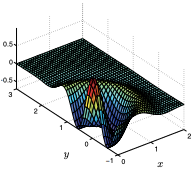
\includegraphics[width=\marginparwidth]{fig62}\captionof{figure}{Plot from Problem $6.1$. The graphic in this figure was created with Matlab. Python\rq s graphics engine is sort of privative in comparison to Matlab\rq s, so you won\rq t get something quite so nice. In particular, getting the scaling right is painful in Python.}}
The wave equation for transverse waves on a rubber sheet is
\begin{equation}\label{eq:62}
\mu \frac{\partial^2 z}{\partial t^2} = \sigma (\frac{\partial^2 z}{\partial x^2} + \frac{\partial^2 z}{\partial y^2} )
\end{equation}
In this equation $\mu$ is the surface mass density of the sheet, with units of mass/area.
The quantity $\sigma$ is the surface tension, which has rather odd units. By inspecting
the equation above you can find that σ has units of force/length, which doesn\rq t
seem right for a surface. But it is, in fact, correct as you can see by performing the
following thought experiment. Cut a slit of length $L$ in the rubber sheet and think
about how much force you have to exert to pull the lips of this slit together. Now
imagine doubling $L$; doesn\rq t it seem that you should have to pull twice as hard to close the slit? Well, if it doesn\rq t, it should; the formula for this closing force is
given by $\sigma L$, which defines the meaning of $\sigma$.
We can solve the two-dimensional wave equation using the same staggered
leapfrog techniques that we used for the one-dimensional case, except now we
need to use a two dimensional grid to represent $z(x, y,t)$. We\rq ll use the notation $ z^n_{j,k} = z(x_j,y_k,t_n) $ to represent the function values. With this notation, the
derivatives can be approximated as
\begin{equation}\label{eq:63}
\frac{\partial^2 z}{\partial t^2} \approx \frac{z^{n+1}_{j,k}-2z^n_{j,k}+z^{n-1}_{j,k}}{\tau^2} )
\end{equation}
\begin{equation}\label{eq:64}
\frac{\partial^2 z}{\partial x^2} \approx \frac{z^{n}_{j+1,k}-2z^n_{j,k}+z^{n}_{j-1,k}}{h^2_x} )
\end{equation}\\
\begin{equation}\label{eq:65}
\frac{\partial^2 z}{\partial y^2} \approx \frac{z^{n}_{j,k+1}-2z^n_{j,k}+z^{n}_{j,k-1}}{h^2_y} )
\end{equation}
where $h_x$ and $h_y$ are the grid spacings in the $x$ and $y$ dimensions. We insert these
three equations into Eq. \eqref{eg:62} to get an expression that we can solve for z at the
next time (i.e. $z^{n+1}_{j,k} $). Then we use this expression along with the discrete version
of the initial velocity condition
\begin{equation}\label{eq:66}
v_0(x_j,y_k)\approx \frac{z^{n+1}_{j,k}-z^{n-1}_{j,k}}{2\tau}
\end{equation}
to find an expression for the initial value of $z^{n-1}_{j,k}$ (i.e. $zold$) so we can get things
started.
\paragraph*{P6.2} 

\begin{enumerate}[label=(\alph*)]
	\item Derive the staggered leapfrog algorithm for the case of square cells
with $h_x = h_y = h$. Write a program that animates the solution of the
two dimensional wave equation on a square region that is $[−5,5] ×
[−5,5]$ and that has fixed edges. Use a cell-edge square grid with
the edge-values pinned to zero to enforce the boundary condition.
Choose $\sigma = 2 N/m$ and $ \mu = 0.3 kg/m^2$
and use a displacement initial
condition that is a Gaussian pulse with zero velocity

\begin{equation}\label{eq:67}
z(x,y,0) = e^{-5(x^2+y^2)}
\end{equation}

This initial condition doesn\rq t strictly satisfy the boundary conditions,
so you should pin the edges to zero.
Getting the animation to work can be tricky, so here is a framework of
code for the animation loop:
\begin{lstlisting}
from mpl_toolkits.mplot3d import Axes3D
import matplotlib.pyplot as plt
import numpy as np
# your code to initialize things
tfinal=10
t=np.arange(0,tfinal,tau)
skip=10
fig = plt.figure(1)
# here is the loop that steps the solution along
for m in range(len(t)):
# Your code to step the solution
# make plots every skip time steps
if m % skip == 0:
plt.clf()
ax = fig.gca(projection='3d')
surf = ax.plot_surface(X,Y,z)
ax.set_zlim(-0.5, 0.5)
plt.xlabel('x')
plt.ylabel('y')
plt.draw()
plt.pause(0.1)
\end{lstlisting}
	\marginpar{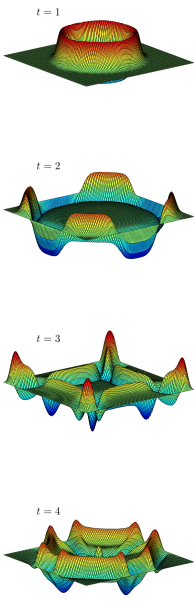
\includegraphics[width=\marginparwidth]{fig63}\captionof{figure}{A wave on a rubber sheet with fixed edges.}}
Run the simulation long enough that you see the effect of repeated
reflections from the edges.
\item You will find that this two-dimensional problem has a Courant condition similar to the one-dimensional case, but with a factor out front:
\begin{equation}\label{eq:68}
\tau < fh \sqrt{\frac{\mu}{\sigma}}
\end{equation}
where $\sqrt{\frac{\mu}{\sigma}}$ is the wave speed and $f$ is an arbitrary constant. Determine the value of the constant $f$ by numerical experimentation.
(Try various values of $\tau$ and discover where the boundary is between
numerical stability and instability.)
\item Also watch what happens at the center of the sheet by making a plot
of $z(0,0,t)$ there. In one dimension the pulse propagates away from
its initial position making that point quickly come to rest with $z = 0$.
This also happens for the three-dimensional wave equation. But
something completely different happens for an even number of dimensions; you should be able to see it in your plot by looking at the
behavior of $z(0,0,t)$ before the first reflection comes back.
\item Finally, change the initial conditions so that the sheet is initially flat
but with the initial velocity given by the Gaussian pulse of Eq. \eqref{eg:67}.
In one dimension when you pulse the system like this the string at
the point of application of the pulse moves up and stays up until
the reflection comes back from the ends of the system. (We did this
experiment with the slinky in Lab 5.) Does the same thing happen
in the middle of the sheet when you apply this initial velocity pulse?
Answer this question by looking at your plot of $z(0,0,t)$. You should
find that the two-dimensional wave equation behaves very differently
from the one-dimensional wave equation.


\end{enumerate}
\section*{Elliptic, hyperbolic, and parabolic PDEs}
\addcontentsline{toc}{section}{Elliptic, hyperbolic, and parabolic PDEs}

Let\rq s step back and look at some general concepts related to solving partial differential equations. Three of the most famous PDEs of classical physics are

\begin{enumerate}[label=(\roman*)]
\item Poisson\rq s equation for the electrostatic potential $V (x, y)$ given the charge
density $ρ(x, y)$
\begin{equation}\label{eq:69}
\frac{\partial^{2} V}{\partial x^{2}}+\frac{\partial^{2} V}{\partial y^{2}}=\frac{-\rho}{\epsilon_{0}}+\text { Boundary Conditions }
\end{equation}
\item The wave equation for the wave displacement $y(x,t)$
\begin{equation}\label{eq:610}
\frac{\partial^{2} y}{\partial x^{2}}-\frac{1}{c^{2}} \frac{\partial^{2} y}{\partial t^{2}}=0+\text { Boundary Conditions }
\end{equation}
\item The thermal diffusion equation for the temperature distribution $T(x,t)$ in a
medium with diffusion coefficient $D$
\begin{equation}\label{eq:611}
\frac{\partial T}{\partial t}=D \frac{\partial^{2} T}{\partial x^{2}}+\text { Boundary Conditions }
\end{equation}
\end{enumerate}
To this point in the course, we\rq ve focused mostly on the wave equation, but over
the next several labs we\rq ll start to tackle some of the other PDEs. \\
Mathematicians have special names for these three types of partial differential
equations, and people who study numerical methods often use these names, so
let\rq s discuss them a bit. The three names are elliptic, hyperbolic, and parabolic.
You can remember which name goes with which of the equations above by remembering the classical formulas for these conic sections:
\begin{equation}\label{eq:612}
\text{ellipse:} \frac{x^{2}}{a^{2}}+\frac{y^{2}}{b^{2}}=1
\end{equation}
\begin{equation}\label{eq:613}
\text{hyperbola:} \frac{x^{2}}{a^{2}}-\frac{y^{2}}{b^{2}}=1
\end{equation}
\begin{equation}\label{eq:614}
\text{parabola:} y=a x^{2}
\end{equation}
Compare these equations with the classical PDE\rq s above and make sure you can use their resemblances to each other to remember the following rules: Poisson\rq s equation is elliptic, the wave equation is hyperbolic, and the diffusion equation is parabolic. These names are important because each different type of equation requires a different type of algorithm and boundary conditions. \\  Elliptic equations require the same kind of boundary conditions as Poisson\rq s equation: $V (x, y)$ specified on all of the surfaces surrounding the region of interest. Notice that there is no time delay in electrostatics. When all of the bounding voltages are specified, Poisson\rq s equation says that $V(x, y)$ is determined instantly throughout the region surrounded by these bounding surfaces. Because of the finite speed of light this is incorrect, but Poisson\rq s equation is a good approximation to use in problems where things happen slowly compared to the time it takes light to cross the computing region. \\
To understand hyperbolic boundary conditions, think about a guitar string
described by the transverse displacement function $y(x,t)$. It makes sense to
give spatial boundary conditions at the two ends of the string, but it makes no
sense to specify conditions at both $t = 0$ and $t = t_{final}$ because we don\rq t know the
displacement in the future. This means that you can\rq t pretend that $(x,t)$ are like
$(x, y)$ in Poisson\rq s equation and use \lq\lq surrounding\rq\rq -type boundary conditions. But
we can see the right thing to do by thinking about what a guitar string does. With
the end positions specified, the motion of the string is determined by giving it an
initial displacement $y(x,0)$ and an initial velocity $\partial y(x,t)/ \partial t\vert_{t=0}$, and then letting
the motion run until we reach the final time. So for hyperbolic equations the
proper boundary conditions are to specify end conditions on y as a function of
time and to specify the initial conditions $y(x,0)$ and $\partial y(x,t)/ \partial t\vert_{t=0}$. \\

Parabolic boundary conditions are similar to hyperbolic ones, but with one difference. Think about a thermally-conducting bar with its ends held at fixed
temperatures. Once again, surrounding-type boundary conditions are inappropriate because we don\rq t want to specify the future. So as in the hyperbolic case,
we can specify conditions at the ends of the bar, but we also want to give initial conditions at $t = 0$. For thermal diffusion we specify the initial temperature
$T (x,0)$, but that\rq s all we need; the \rq\rq velocity\lq\lq $\partial T / \partial t$ is determined by Eq. \eqref{eg:611},
so it makes no sense to give it as a separate boundary condition. Summarizing:
for parabolic equations we specify end conditions and a single initial condition
$T (x,0)$ rather than the two required by hyperbolic equations. \\ 

If this seems like an arcane side trip into theory, we\rq re sorry, but it\rq s important.
When you numerically solve partial differential equations you will spend 10 \%
of your time coding the equation itself and 90 \% of your time trying to make the
boundary conditions work. It\rq s important to understand what the appropriate
boundary conditions are. \\
Finally, there are many more partial differential equations in physics than
just these three. Nevertheless, if you clearly understand these basic cases you
can usually tell what boundary conditions to use when you encounter a new one.
Here, for instance, is Schr{\"o}dinger\rq s equation:
\begin{equation}\label{eq:615}
i \bar{h} \frac{\partial \psi}{\partial t}=-\frac{\bar{h}^{2}}{2 m} \frac{\partial^{2} \psi}{\partial x^{2}} + V \psi
\end{equation}
which is the basic equation of quantum (or \rq\rq wave\lq\lq) mechanics. The wavy nature
of the physics described by this equation might lead you to think that the proper
boundary conditions on $\psi (x,t)$ would be hyperbolic: end conditions on $\psi$ and initial conditions on $\psi$ and $\partial \psi / \partial t$. But if you look at the form of the equation, it
looks like thermal diffusion. Looks are not misleading here; to solve this equation
you only need to specify $\psi$ at the ends in x and the initial distribution $ \psi(x,0)$, but
not its time derivative. And what are you supposed to do when your system is both hyperbolic and
parabolic, like the wave equation with damping?
\begin{equation}\label{eq:616}
\frac{\partial^{2} y}{\partial x^{2}}-\frac{1}{c^{2}} \frac{\partial^{2} y}{\partial t^{2}}-\frac{1}{D} \frac{\partial y}{\partial t}=0
\end{equation}
The rule is that the highest-order time derivative wins, so this equation needs
hyperbolic boundary conditions
\paragraph*{P6.3} Make sure you understand this material well enough that you are comfortable answering basic questions about PDE types and what types of
boundary conditions go with them on a quiz and/or an exam. Then explain
it to the TA to pass this problem off.


\chapter*{The Diffusion Equation and Implicit Methods}
\addcontentsline{toc}{chapter}{The Diffusion Equation and Implicit Methods} 
\section*{Analytic approach to the Diffusion Equation}
\addcontentsline{toc}{section}{Analytic approach to the Diffusion Equation} 

Now let\rq s attack the diffusion equation
\begin{equation}\label{eq:71}
\frac{\partial T}{\partial t}=D \frac{\partial^{2} T}{\partial x^{2}}
\end{equation}
This equation describes how the distribution $T$ (often temperature) diffuses
through a material with a constant diffusion coefficient $D$. The diffusion equation
can be approached analytically via separation of variables by assuming that T is
of the form $T(x,t) = g(x)f(t)$. Plugging this form into the diffusion equation, we
find
\begin{equation}\label{eq:72}
\frac{1}{D} \frac{\dot{f}(t)}{f(t)}=\frac{g^{\prime \prime}(x)}{g(x)}
\end{equation}
The left-hand side depends only on time, while the right-hand side depends only
on space, so both sides must equal a constant, say $-a^2$. Thus, $f (t)$ must satisfy
\begin{equation}\label{eq:73}
\dot{f}(t)=-\gamma f(t)
\end{equation}
where $ \gamma = a^2 D$ so that $f(t)$ is
\begin{equation}\label{eq:74}
f(t)=e^{-\gamma t}
\end{equation}
Meanwhile $g(x)$ must satisfy
\begin{equation}\label{eq:75}
g^{\prime \prime}(x)+a^{2} g(x)=0
\end{equation}
If we specify edge-value boundary conditions so that $T(x = 0,t) = 0$ and $T(x =
L,t) = 0$ then the solution to Eq. \eqref{eg:75} is simply
\begin{equation}\label{eq:76}
g(x) = \sin(ax)
\end{equation}

and the separation constant can take on the values $a = n \pi /L$, where n is an integer.
Any initial distribution $T(x,t = 0)$ that satisfies these boundary conditions can be
composed by summing these sine functions with different weights using Fourier
series techniques. Notice that higher spatial frequencies (i.e. large $n$) damp faster,
according to Eq. \eqref{eg:74}. We already studied how to use separation of variables
computationally in the first several labs of this manual, so let\rq s move directly to
time-stepping methods for solving the diffusion equation.

\section*{Numerical approach: a first try}
\addcontentsline{toc}{section}{Numerical approach: a first try} 

Let\rq s try to solve the diffusion equation on a grid as we did with the wave equation.
If we finite difference the diffusion equation using a centered time derivative and
a centered second derivative in $x$ we get
\begin{equation}\label{eq:77}
\frac{T_{j}^{n+1}-T_{j}^{n-1}}{2 \tau}=\frac{D}{h^{2}}\left(T_{j+1}^{n}-2 T_{j}^{n}+T_{j-1}^{n}\right)
\end{equation}
Solving for $T_j^{n+1}$ to obtain an algorithm similar to leapfrog then gives

\begin{equation}\label{eq:78}
T_{j}^{n+1}=T_{j}^{n-1}+\frac{2 D \tau}{h^{2}}\left(T_{j+1}^{n}-2 T_{j}^{n}+T_{j-1}^{n}\right)
\end{equation}
There is a problem starting this algorithm because of the need to have T one time
step in the past ($T_j^{n+1}$), but even after we work around this problem this algorithm
turns out to be worthless. We won\rq t make you code it up, but if you did, you\rq d
find that no matter how small a time step $\tau$ you choose, you encounter the same
kind of instability that plagues staggered leapfrog when the step size got too big
(infinite zig-zags). Such an algorithm is called unconditionally unstable, and is an
invitation to keep looking. This must have been a nasty surprise for the pioneers
of numerical analysis who first encountered it. \\ 
For now, let\rq s sacrifice second-order accuracy to obtain a stable algorithm. If
we don\rq t center the time derivative, but use instead a forward difference we find
\begin{equation}\label{eq:79}
\frac{T_{j}^{n+1}-T_{j}^{n}}{\tau}=\frac{D}{h^{2}}\left(T_{j+1}^{n}-2 T_{j}^{n}+T_{j-1}^{n}\right)
\end{equation}
This algorithm has problems since the left side of Eq. (7.9) is centered at time $t_{n+/frac{1}{2}}$,while the right side is centered at time $t_n$. This makes the algorithm inaccurate, but it turns out that it is stable if $\tau$ is small enough. Solving for $T_j^{n+1}$ yields
\begin{equation}\label{eq:710}
T_{j}^{n+1}=T_{j}^{n}+\frac{D \tau}{h^{2}}\left(T_{j+1}^{n}-2 T_{j}^{n}+T_{j-1}^{n}\right)
\end{equation}
\paragraph*{P7.1}
	\marginpar{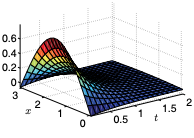
\includegraphics[width=\marginparwidth]{fig71}\captionof{figure}{Diffusion of the $n=$ 1 sine temperature distribution given in Problem 7.1(a).}}
\begin{enumerate}[label=(\alph*)]
\item 
Modify one of your staggered leapfrog programs that uses a cell-center
grid to implement Eq. \eqref{eg:710} to solve the diffusion equation on the
interval $[0,L]$ with initial distribution
\begin{equation}\label{eq:711}
T(x, 0)=\sin (\pi x / L)
\end{equation}

and boundary conditions $ T(0) = T (L) = 0$. Use $D = 2$, $L = 3$, and $N =
20$. You don\rq t need to make a space-time surface plot like Fig. 7.1. Just
make a line plot that updates each time step as we\rq ve done previously.
This algorithm has a CFL condition on the time step $\tau$ of the form

\begin{equation}\label{eq:712}
\tau \leq C \frac{h^{2}}{D}
\end{equation}
Determine the value of $C$ by numerical experimentation.
Test the accuracy of your numerical solution by overlaying a graph of
the analytic solution. Plot the numerical solution as points and the
exact solution as a line so you can tell the difference. Show that your
grid solution matches the exact solution with increasing accuracy as
the number of grid points $N$ is increased from 20 to 40 and then to 80.
You can calculate the RMS error using something like
\begin{lstlisting}
error = np.sqrt( np.mean( (T - exact)**2 ))
\end{lstlisting}

\item Get a feel for what the diffusion coefficient does by trying several
different values for $D$ in your code. Give a physical description of this
parameter to the TA.
\item Now switch your boundary conditions to be insulating, with $\partial T / \partial x=
0$ at both ends. Explain what these two types of boundary conditions
mean by thinking about a watermelon that is warmer in the middle
than at the edge. Tell physically how you would impose both of these
boundary conditions (specifying the value and specifying the derivative) on the watermelon and explain what the temperature history of
the watermelon has to do with your plots of $T(x)$ vs. time.
\end{enumerate}
	\marginpar{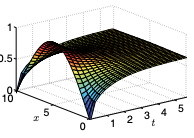
\includegraphics[width=\marginparwidth]{fig72}\captionof{figure}{Diffusion of the Gaussian temperature distribution given in Problem 7.1 (c) with insulating boundary conditions.}}
Even though this technique can give us OK results, the time step constraint for this
method is onerous. The constraint is of the form $\tau < C h^2$, where $C$ is a constant.
Suppose, for instance, that to resolve some spatial feature you need to decrease $h$
by a factor of 5; then you will have to decrease $\tau$ by a factor of 25. This will make
your code take forever to run, which motivates us to find a better way

\section*{Implicit Methods: the Crank-Nicolson Algorithm}
\addcontentsline{toc}{section}{Implicit Methods: the Crank-Nicolson Algorithm} 

The time-stepping algorithms we have discussed so far are of the same type: at
each spatial grid point $j$ you use present, and perhaps past, values of $y(x,t)$ at that
grid point and at neighboring grid points to find the future $y(x,t)$ at $j$. Methods
like this, that depend in a simple way on present and past values to predict future
values, are said to be $explicit$ and are easy to code. They are also often numerically
unstable, or have severe constraints on the size of the time step.\\
$Implicit$ methods are generally harder to implement than explicit methods,
but they have much better stability properties. The reason they are harder is that
they assume that you already know the future. To give you a better feel for what\rq\rq implicit\lq\lq means, let\rq s study the simple first-order differential equation

\begin{equation}\label{eq:713}
\frac{dy}{dt	} = -y
\end{equation}
\paragraph*{P7.2}
\begin{enumerate}[label=(\alph*)]
\item Write a program to solve this equation using Euler\rq s method:
\begin{equation}\label{eq:714}
\frac{y_{n+1}-y_n}{\tau} = -y_n
\end{equation}
The program to solve for $y$ using Euler\rq s method is only a few lines of
code (like less than 10 lines, including the plot command). Here are
the first few lines:
\begin{lstlisting}
tau = 0.5
tmax = 20.
t = np.arange(0,tmax,tau)
y = np.zeros_like(t)
\end{lstlisting}
	\marginpar{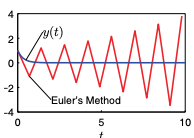
\includegraphics[width=\marginparwidth]{fig73}\captionof{figure}{Euler\rq s method is unstable for $\tau>2 .$ ( $\tau=2.1$ in this case.)}}
Show by numerical experimentation that Euler\rq s method is unstable
for large $\tau$ . You should find that the algorithm that is unstable if $\tau > 2$.
Use $y(0) = 1$ as your initial condition. This is an example of an explicit
\item Notice that the left side of Eq. \eqref{eg:714} is centered on time $t_{n+\frac{1}{2}}$ but the
right side is centered on $t_n$. Fix this by centering the right-hand side at time $t_{n+\frac{1}{2}}$ by using an average of the advanced and current values of $y$, method.
\begin{equation*}
y_{n} \Rightarrow \frac{y_{n}+y_{n+1}}{2}
\end{equation*}
Modify your program to implement this fix, then show by numerical
experimentation that when $\tau$ becomes large this method doesn\rq t blow
up. It isn\rq t correct because $y_n$ bounces between positive and negative
values, but at least it doesn\rq t blow up. The presence of $\tau$ in the denominator is the tip-off that this is an implicit method, and the improved
stability is the point of using something implicit.

	\marginpar{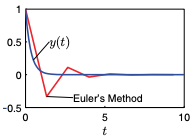
\includegraphics[width=\marginparwidth]{fig74}\captionof{figure}{Euler\rq s method is unstable for $\tau>2 .$ ( $\tau=2.1$ in this case.)}}
\item  Now Modify Euler\rq s method by making it fully implicit by using $y_{n+1}$
in place of $y_n$ on the right side of Eq. \eqref{eg:714} (this makes both sides of
the equation reach into the future). This method is no more accurate
than Euler\rq s method for small time steps, but it is much more stable
and it doesn\rq t bounce between positive and negative values.
Show by numerical experimentation in a modified program that this
fully implicit method damps even when $ \tau $ is large. For instance, see
what happens if you choose $ \tau = 5$ with a final time of 20 seconds. The
time-centered method of part (b) would bounce and damp, but you
should see that the fully implicit method just damps. It\rq s terribly inaccurate, and actually doesn\rq t even damp as fast as the exact solution,
but at least it doesn\rq t bounce like part (b) or go to infinity like part (a).
Methods like this are said to be \rq\rq absolutely stable\lq\lq. Of course, it makes
no sense to choose really large time steps, like $ \tau = 100$ when you only
want to run the solution out to 10 seconds.

	\marginpar{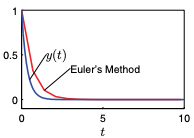
\includegraphics[width=\marginparwidth]{fig75}\captionof{figure}{The fully implicit method in $7.2(\mathrm{c})$ with $\tau=2.1$.}}
\end{enumerate}

\section*{The diffusion equation with Crank-Nicolson}
\addcontentsline{toc}{section}{The diffusion equation with Crank-Nicolson} 
	\marginpar{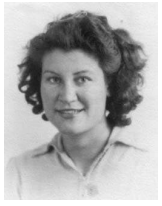
\includegraphics[width=\marginparwidth]{nicolson}\captionof{figure}{Phyllis Nicolson (1917-1968, English)}}
		\marginpar{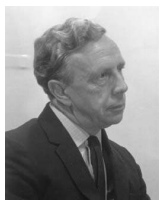
\includegraphics[width=\marginparwidth]{crank}\captionof{figure}{John Crank (1916-2006, English)}}

Now let\rq s look at the diffusion equation again and see how implicit methods can
help us find a stable numerical algorithm. Here\rq s the equation again
\begin{equation}\label{eq:715}
\frac{\partial T}{\partial t}=D \frac{\partial^{2} T}{\partial x^{2}}
\end{equation}
We begin by finite differencing the right side as usual:

\begin{equation}\label{eq:716}
\frac{\partial T_{j}}{\partial t}=D \frac{T_{j+1}-2 T_{j}+T_{j-1}}{h^{2}}
\end{equation}
Now we discretize the time derivative by taking a forward time derivative on the
left:
\begin{equation}\label{eq:717}
\frac{T_{j}^{n+1}-T_{j}^{n}}{\tau}=D \frac{T_{j+1}^{n}-2 T_{j}^{n}+T_{j-1}^{n}}{h^{2}}
\end{equation}
This puts the left side of the equation at time level $t_{n+\frac{1}{2}}$, while the right side is
at tn. To put the right side at the same time level (so that the algorithm will be
second-order accurate), we replace each occurrence of $T$ on the right-hand side
by the average
\begin{equation}\label{eq:718}
T^{n+\frac{1}{2}}=\frac{T^{n+1}+T^{n}}{2}
\end{equation}
like this:
\begin{equation}\label{eq:719}
\frac{T_{j}^{n+1}-T_{j}^{n}}{\tau}=D \frac{T_{j+1}^{n+1}+T_{j+1}^{n}-2 T_{j}^{n+1}-2 T_{j}^{n}+T_{j-1}^{n+1}+T_{j-1}^{n}}{2 h^{2}}
\end{equation}
If you look carefully at this equation you will see that there is a problem: how are
we supposed to solve for $T^{n+1}_j$? The future values $T^{n+1}$are all over the place, and
they involve three neighboring grid points ($T^{n+1}_{j-1}$ , $T^{n+1}_{j}$, and $T^{n+1}_{j+1}$) so we can’t just
solve in a simple way for $T^{n+1}_j$. This is an example of why implicit methods are
harder than explicit methods. \\ 
In the hope that something useful will turn up, let\rq s put all of the variables at
time level $n +1$ on the left, and all of the ones at level n on the right.
\begin{equation}\label{eq:720}
-T_{j-1}^{n+1}+\left(\frac{2 h^{2}}{\tau D}+2\right) T_{j}^{n+1}-T_{j+1}^{n+1}=T_{j-1}^{n}+\left(\frac{2 h^{2}}{\tau D}-2\right) T_{j}^{n}+T_{j+1}^{n}
\end{equation}
We know this looks ugly, but it really isn\rq t so bad. To solve for $T^{n+1}_j$we just need to
solve a linear system, as we did in Lab 2 on two-point boundary value problems.
When a system of equations must be solved to find the future values, we say
that the method is implicit. This particular implicit method is called the CrankNicolson algorithm. \\ 
To see more clearly what we are doing, and to make the algorithm a bit more
efficient, let\rq s define a matrix A to describe the left side of Eq. \eqref{eg:720} and another
matrix B to describe the right side, like this:
\begin{equation}\label{eq:721}
\mathbf{A} T^{n+1}=\mathbf{B} T^{n}
\end{equation}
T is now a column vector. The elements of A are given by\\
\begin{equation*}
A_{j, k}=0 except for : 
\end{equation*}
\begin{equation}\label{eq:722}
A_{j, j-1}=-1 ; \quad A_{j, j}=\frac{2 h^{2}}{\tau D}+2 ; A_{j, j+1}=-1
\end{equation}
and the elements of B are given by
\begin{equation*}
B_{j, k}=0 except for : 
\end{equation*}
\begin{equation}\label{eq:723}
B_{j, j-1}=-1 ; \quad B_{j, j}=\frac{2 h^{2}}{\tau D}-2 ; B_{j, j+1}=1
\end{equation}
Once the boundary conditions are added to these matrices, Eq. \eqref{eg:721} could be
solved symbolically to find $T^{n+1}$
\begin{equation}\label{eq:724}
T^{n+1}=\mathbf{A}^{-1} \mathbf{B} T^{n}
\end{equation}
However, since inverting a matrix is computationally expensive we will use Gauss
elimination instead as we did in lab 2 (with SciPy\rq s linalg.solve function). Here
is a sketch of how you would implement the Crank-Nicolson algorithm in Python.
\begin{itemize}
\item Load the matrices A and B as given in Eq. \eqref{eg:722} and Eq. \eqref{eg:723} for all of
the rows except the first and last. Since the diffusion coefficient D doesn\rq t
change with time you can load A and B just once before the time loop starts.
\item The first and last rows involve the boundary conditions. Usually it is easier
to handle the boundary conditions if we plan to do the linear solve of our matrix equation $\mathbf{A} T^{n+1}=\mathbf{B} T^{n}$ in two steps, like this:
\begin{lstlisting}
import scipy.linalg as la
# matrix multiply to get the right-hand side
r = B@T
# set r as appropriate for the boundary conditions
r[0] = ...
r[-1] = ...
# Solve AT = r. The T we get is for the next time step.
# We don't need to keep track of previous T values, so just
# load the new T directly into T itself
T = la.solve(A,r)
\end{lstlisting}
With this code we can just load the top and bottom rows of B with zeros, creating a right-hand-side vector $r$ with zeros in the top and bottom positions.
The top and bottom rows of A can then be loaded with the appropriate
terms to enforce the desired boundary conditions on $T^{n+1}$, and the top and
bottom positions of r can be loaded as required just before the linear solve,
as indicated above. For example, if the boundary conditions were $T (0) = 1$ and $T (L) = 5$, the top
and bottom rows of A and the top and bottom positions of $r$ would have
been loaded like this (assuming a cell-center grid with ghost points):
\begin{lstlisting}
# Set the A portion up where you define the matrix
A[0,0] = 0.5
A[0,1] = 0.5
A[-1,-1] = 0.5
A[-1,-2] = 0.5
... # skipped code
# Set the r portion of the boundary condition
# down in the time loop for each iteration
r[0] = 1
r[-1] = 5
\end{lstlisting}
so that the equations for the top and bottom rows are
\begin{equation}\label{eq:725}
\frac{T_{0}+T_{1}}{2}=r_{0} \quad \frac{T_{N}+T_{N+1}}{2}=r_{N+1}
\end{equation}
The matrix B just stays out of the way (is zero) in the top and bottom rows.
\item  Once the matrices A and B are loaded, finding the new temperature inside the time loop is accomplished in the time loop by solving the matrix
equation using the code fragment listed above.
\end{itemize}
\paragraph*{P7.3}
\begin{enumerate}[label=(\alph*)]
\item Write program that implements the Crank-Nicolson algorithm with
fixed-edge boundary conditions, $T(0) = 0$ and $T(L) = 0$. Test your
program by running it with $D = 2$ and an initial temperature given
by $T (x) = sin(\pi x/L$). Try various values of $\tau$ and see how it compares
with the exact solution. Verify that when the time step is too large the
solution is inaccurate, but still stable. To do the checks at large time
step you will need to use a long run time and not skip any steps in the
plotting.
\item  Now study the accuracy of this algorithm by using various values of
the cell number $N$ and the time step $\tau$. For each pair of choices run
for $t = 5$ s and find the maximum difference between the exact and
numerical solutions. You should find that the time step $\tau$ matters less
than $N$. The number of cells $N$ is the more important parameter for
high accuracy in diffusion problems solved with Crank-Nicolson.

\item Modify the Crank-Nicolson program to use boundary conditions
$ \partial T /\partial x = 0$ at the ends. Run with the same initial condition as in
part (a) (which does not satisfy these boundary conditions) and watch
what happens. Zoom in on the plots early in time to see what happens
in the first few grid points during the first few time steps.
	\marginpar{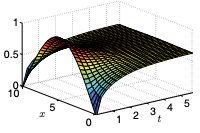
\includegraphics[width=\marginparwidth]{fig76}\captionof{figure}{Solution to 7.3(c)}}
\end{enumerate}

\chapter*{Schr{\"o}dinger\rq s Equation}
\addcontentsline{toc}{chapter}{Schr{\"o}dinger\rq s Equation} 
\section*{Derivations}
\addcontentsline{toc}{section}{Derivations} 

	\marginpar{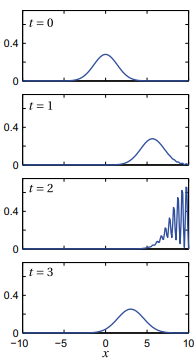
\includegraphics[width=\marginparwidth]{fig81}\captionof{figure}{The probability density $|\psi(x)|^{2}$ of a particle in a box that initially moves to the right and then interferes with itself as it reflects from an infinite potential (Problem 8.2(a)).}}
Here is the time-dependent Schr{\"o}dinger equation which governs the way a quantum wave function changes with time in a one-dimensional potential well $V(x)$:
\begin{equation}\label{eq:81}
i \bar{h} \frac{\partial \psi}{\partial t}=-\frac{\bar{h}^{2}}{2 m} \frac{\partial^{2} \psi}{\partial x^{2}}+V(x) \psi
\end{equation}
Note that except for the presence of the imaginary unit i, this is very much like
the diffusion equation. In fact, a good way to solve it is with the Crank-Nicolson
algorithm. Not only is this algorithm stable for Schr{\"o}dinger\rq s equation, but it has
another important property: it conserves probability. This is very important. If
the algorithm you use does not have this property, then as $\psi$ for a single particle
is advanced in time you have (after a while) 3/4 of a particle, then 1/2, etc. \\
\marginpar{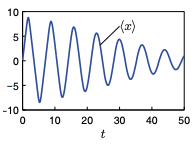
\includegraphics[width=\marginparwidth]{fig82}\captionof{figure}{The expectation position $\langle x\rangle$ for the particle in Fig. 8.1 as time progresses and the packet spreads out (Problem 8.2(c)).}}
The Schr{\"o}dinger equation usually describes the behavior of very tiny things
on very short timescales, so SI quantities like kilograms, meters, and Joules are
essentially infinite in quantum mechanics. Instead, we\rq ll use a system of units
called atomic units. In this system, lengths are measured in units of $a_0$ (the Bohr
radius, $a_0 = 5.29×10^{−11}$), masses are measured in units of the electron mass me ,
energies are measured in units of $E_0$ ($E_0 = \alpha^2mc^2 \approx 27 eV$), and time is measured
in units of $t_0 (t_0 = 24.2 attoseconds)$. These base units are chosen so that the
constants $\bar{h}$ and $m$ both have the numerical value of 1 (e.g. $m = 1m_e$ for an electron).
\paragraph*{P8.1}
Use paper and pencil to derive a Crank-Nicolson algorithm to solve the
Schr{\"o}dinger equation. It will probably be helpful to use the material in
Lab 7 as a guide (beginning with Eq. \eqref{eg:715}). Make sure the $V(x)\psi$ term
enters the algorithm correctly
\section*{Particle in a box}
\addcontentsline{toc}{section}{Particle in a box} 
Let\rq s use this algorithm for solving Schr{\"o}dinger\rq s equation to study the evolution
of a particle in a box with
\begin{equation}\label{eq:82}
V(x)= \begin{cases}0 & \text { if }-L<x<L \\ +\infty & \text { otherwise }\end{cases}
\end{equation}
The infinite potential at the box edges is imposed by forcing the wave function to
be zero at these points:
\begin{equation}\label{eq:83}
\psi(-L)=0 \quad ; \quad \psi(L)=0
\end{equation}

\paragraph*{P8.2}
\marginpar{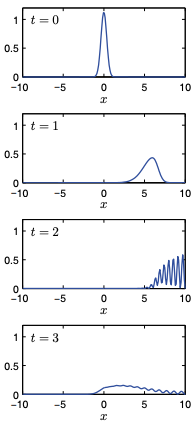
\includegraphics[width=\marginparwidth]{fig83}\captionof{figure}{The probability density $|\psi(x)|^{2}$ of a particle that is initially more localized quickly spreads (Problem 8.2(d)).}}
Modify one of your programs from Lab 7 to implement the Crank-Nicolson algorithm derived above for the case of a particle in a box with $L = 10$. Note we are doing quantum mechanics and the imaginary parts matter now. When assigning complex variables in NumPy, you use the engineering complex number $j$, like this:
\begin{lstlisting}
a = 1.0 + 0.5j
\end{lstlisting}
When you allocate your arrays, you\rq ll need to specify up-front that they will
hold complex values, like this:
\begin{lstlisting}
A = np.zeros((N,N),dtype=np.complex_)
B = np.zeros_like(A,dtype=np.complex_)
\end{lstlisting}
\marginpar{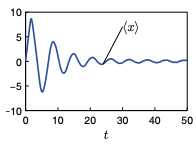
\includegraphics[width=\marginparwidth]{fig84}\captionof{figure}{The expectation position of the particle in Fig. 8.3 as time progresses.}}
\begin{enumerate}[label=(\alph*)]
	\item  Write a script to solve the time-dependent Schr{\"o}dinger equation using
Crank-Nicolson. We find that a cell-edge grid is easiest, but you can
also do cell-center with ghost points if you like. Start with a localized
wave packet of width $\sigma$ and momentum $p$:

\begin{equation}\label{eq:84}
\psi(x, 0)=\frac{1}{\sqrt{\sigma \sqrt{\pi}}} e^{i p x / \bar{h}} e^{-x^{2} /\left(2 \sigma^{2}\right)}
\end{equation}
with $p = 2\pi$ and $\sigma = 2$. (Remember that $ \bar{h}$ in \eqref{eg:84} has the numerical
value of 1 in our units.) This initial condition does not exactly satisfy
the boundary conditions, but it is very close. Check to see how far
off it is at the boundary, and decide how the sizes of $L$ and σ must
compare in to use this initial condition.
Run the script with $N = 200$ and watch the particle (wave packet)
bounce back and forth in the well. Plot the real part of $\psi$ as an animation to visualize the spatial oscillation of the wave packet, then
plot an animation of $\psi * \psi$  so that you can visualize the probability
distribution of the particle. Try switching the sign of $p$ and see what
happens.
\item Verify by doing a numerical integral that $\psi(x,0)$ in the formula given
above is properly normalized. Then run the script and check that
the wave packet stays properly normalized, even though the wave
function is bouncing and spreading within the well. If you are on a
cell-edge grid you should do the integrals with NumPy\rq s trapz rather
than sum.
\item Run the script and verify by numerical integration that the expectation
value of the particle position
\begin{equation}\label{eq:85}
\langle x\rangle=\int_{-L}^{L} \psi^{*}(x, t) x \psi(x, t) d x
\end{equation}
is correct for a bouncing particle. Plot $<x>(t)$ to see the bouncing
behavior. Run long enough that the wave packet spreading modifies
the bouncing to something more like a harmonic oscillator. (Note:
you will only see bouncing-particle behavior until the wave packet
spreads enough to start filling the entire well.)
\item You may be annoyed that the particle spreads out so much in time.
Try to fix this problem by narrowing the wave packet (decrease the
value of $\sigma$ ) so the particle is more localized. Run the script and explain
what you see in terms of quantum mechanics.


\end{enumerate}
\section*{Tunneling}
\addcontentsline{toc}{section}{Tunneling} 
	\marginpar{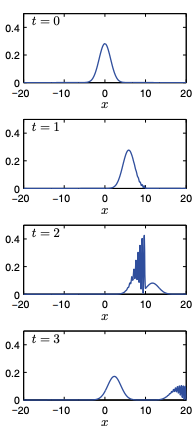
\includegraphics[width=\marginparwidth]{fig85}\captionof{figure}{he probability distribution $|\psi(x)|^{2}$ for a particle incident on a narrow potential barrier located just before $x=10$ with $\left.V_{0}\right\rangle\langle E\rangle$. Part of the wave tunnels through the barrier and part interferes with itself as it is reflected.}}
Now we will allow the pulse to collide with a with a non-infinite potential barrier
of height $V_0$ and width $\delta x = 0.02L$, and study what happens. Classically, the
answer is simple: if the particle has a kinetic energy less than $V_0$ it will be unable
to get over the barrier, but if its kinetic energy is greater than $V_0$ it will slow down
as it passes over the barrier, then resume its normal speed in the region beyond
the barrier. (Think of a ball rolling over a bump on a frictionless track.) Can
the particle get past a barrier that is higher than its kinetic energy in quantum
mechanics? The answer is yes, and this effect is called tunneling. \\ 
To see how the classical picture is modified in quantum mechanics we must
first compute the energy of our pulse so we can compare it to the height of the
barrier. The quantum mechanical formula for the expectation value of the energy
is
\begin{equation}\label{eq:86}
\langle E\rangle=\int_{-\infty}^{\infty} \psi^{*} H \psi d x
\end{equation}
where $\psi^∗$ is the complex conjugate of $\psi$ and where
\begin{equation}\label{eq:87}
H \psi=-\frac{\bar{h}^{2}}{2 m} \frac{\partial^{2} \psi}{\partial x^{2}}+V(x) \psi(x)
\end{equation}
In our case the initial wave function $\psi(x,0)$ given by Eq. \eqref{eg:84} is essentially zero at
the location of the potential barrier, so we may take $V(x) = 0$ in the integral when
we compute the initial energy. Performing the integral, we find
\begin{equation}\label{eq:88}
\langle E\rangle=\frac{p^{2}}{2 m}+\frac{\bar{h}^{2}}{4 m \sigma^{2}}
\end{equation}
Since this is a conservative system, the energy should remain constant throughout
the propagation.
\paragraph*{P8.3}
\begin{enumerate}[label=(\alph*)]
	\item Modify your script from Problem 8.2 so that it uses a computing region hat goes from $-2L$ to $3L$ and a potential
\begin{equation}\label{eq:89}
V(x)= \begin{cases}0 & \text { if }-2 L<x<0.98 L \\ V_{0} & \text { if } 0.98 L \leq x \leq L \\ 0 & \text { if } L<x<3 L \\ +\infty & \text { otherwise }\end{cases}
\end{equation}
so that we have a square potential hill $V(x) = V_0$ between $x = 0.98L$ and $x = L$ and $V = 0$ everywhere else in the well.
Note: Since $V(x)$ was just zero in the last problem, this is the first time
to check if your $V(x)$ terms in Crank-Nicolson are right. If you see
strange behavior, you might want to look at these terms in your code.
\item Run your script several times, varying the height $V_0$ from less than your pulse energy to more than your pulse energy. Overlay a plot
of $V(x)/V_0$ on your plot of $ \vert \psi\vert^2$ and look at the behavior of $\psi$ in the barrier region. You should do several experiments with your code. (1) Try making
the barrier height both higher than your initial energy and lower than
your initial energy. Explain to your TA how the quantum behavior
differs from classical behavior. You should find that even when the
barrier is low enough that a classical particle could get over it, some
particles still come back. (2) Experiment with the width of your barrier
and see what its effect is on how many particles tunnel through. As
part of this experiment, figure out a way to calculate what fraction of
the particles make it through the barrier.

\end{enumerate}
\chapter*{Poisson\rq s Equation: Iteration Methods}
\addcontentsline{toc}{chapter}{Poisson\rq  s Equation: Iteration Methods} 
In three dimensions, Poisson\rq s equation is given by
\begin{equation}\label{eq:91}
\frac{\partial^{2} V}{\partial x^{2}}+\frac{\partial^{2} V}{\partial y^{2}}+\frac{\partial^{2} V}{\partial z^{2}}=-\frac{\rho}{\epsilon_{0}}
\end{equation}
Poisson\rq s equation is used to describe the electric potential in a region of space
with charge density described by $ρ:^1$ You can solve the full 3D equation using
the technique we teach you in this lab, but we won’t make you do that here.
Instead, we’ll focus on geometries that are infinitely long in the $z$-dimension with
a constant cross-section in the $x - y$ plane. In these cases the z derivative goes to
zero, and Poisson\rq s equation reduces to
\begin{equation}\label{eq:92}
\frac{\partial^{2} V}{\partial x^{2}}+\frac{\partial^{2} V}{\partial y^{2}}=-\frac{\rho}{\epsilon_{0}}
\end{equation}
Note that by studying this equation we are also studying Laplace\rq s equation (Poisson\rq s equation with $\rho = 0$) and the steady state solutions to the diffusion equation
in two dimensions ($\partial T / \partial t = 0$ in steady state).


\section*{Finite difference form}
\addcontentsline{toc}{section}{Finite difference form}
The first step in numerically solving Poisson\rq s equation is to define a 2-D spatial grid. For simplicity, we\rq ll use a rectangular grid where the x coordinate is represented by $N_x$ values $x_j$ equally spaced with step size $h_x$ , and the y coordinate is represented by $N_y$ values $y_k$ equally spaced with step size hy . This
creates a rectangular grid with $N_x × N_y$ grid points, just as we used in Lab 6 for
the 2-d wave equation. We\rq ll denote the potential on this grid using the notation $V(x_j,y_k) = V_{j,k}$ \\
The second step is to write down the finite-difference approximation to the
second derivatives in Poisson\rq s equation to obtain a grid-based version of Poisson\rq s
equation. In our notation, Poisson\rq s equation is the represented by
\begin{equation}\label{eq:93}
\frac{V_{j+1, k}-2 V_{j, k}+V_{j-1, k}}{h_{x}^{2}}+\frac{V_{j, k+1}-2 V_{j, k}+V_{j, k-1}}{h_{y}^{2}}=-\frac{\rho_{j, k}}{\epsilon_{0}}
\end{equation}

This set of equations can only be used at interior grid points because on the edges
it reaches beyond the grid, but this is OK because the boundary conditions tell us
what $V$ is on the edges of the region.
\\
Equation \eqref{eg:93} plus the boundary conditions represent a set of linear equations for the unknowns $V_{j,k}$ , so we could imagine just doing a big linear solve to
find $V$ all at once. Because this sounds so simple, let\rq s explore it a little to see why
we are not going to pursue this idea. The number of unknowns $V_{j,k}$ is $N_x × N_y$ ,
which for a 100 $×$ 100 grid is 10,000 unknowns. So to do the solve directly we would
have to be working with a 10,000 $×$ 10,000 matrix, requiring 800 megabytes of RAM
to store the matrix. Doing this big solve is possible for 2-dimensional problems
like this because computers with much more memory than this are common.
However, for larger grids the matrices can quickly get out of hand. Furthermore,
if you wanted to do a 3-dimensional solve for a 100 $×$ 100 $×$ 100 grid, this would
require $(10^4)^3 × 8 = 8 × 10^{12}$, or about 8 terabytes of memory. Computers like this
are becoming possible, but this is still a tiny computational grid. So even though
computers with large amounts of RAM are becoming common, people still use
iteration methods like the ones we are about to describe.

\section*{Iteration method on a simple example}
\addcontentsline{toc}{section}{Iteration method on a simple example}
Consider solving this equation:

\begin{equation}\label{eq:94}
x = e^{-x}
\end{equation}
One method to solve this equation is to make a guess for the solution, call it $x_0$,
and then iterate on the equation like this:
\begin{equation}\label{eq:95}
x_{n+1}=e^{-x_{n}}
\end{equation}
For large values of $n$, we find that the process converges to the exact solution
$ \bar{x} = 0.567$. Let\rq s do a little analysis to see why it works. Let $\bar{x}$ be the exact solution
of this equation and suppose that at the $n^{th}$ iteration level we are close to the
solution, only missing it by the small quantity $\delta n$ like this: $x_n = \bar{x} + \delta n$. Let\rq s
substitute this approximate solution into Eq. \eqref{eg:95} and expand using a Taylor
series. Recall that the general form for a Taylor\rq s series is
\begin{equation}\label{eq:96}
f(x+h)=f(x)+f^{\prime}(x) h+\frac{1}{2} f^{\prime \prime}(x) h^{2}+\cdots+f^{(n)}(x) \frac{h^{n}}{n !}+\cdots
\end{equation}

When we substitute our approximate solution into 
Eq. \eqref{eq:95} and 
expand around the exact solution $ \bar{x} $ we get

\begin{equation}\label{eq:97}
f(x_{n+1}=e^{-\bar{x}-\delta_{n}} \approx e^{-\bar{x}}-\delta_{n} e^{-\bar{x}}+\cdots
\end{equation}

If we ignore the terms that are higher order in $\delta$ (represented by ···), then Eq. \eqref{eg:97}
shows that the error at the next iteration step is $\delta_{n+1} = −e^{−\bar{x}}\delta_n$. When we are close
to the solution the error becomes smaller every iteration by the factor $−e^{-\bar{x}}$. Since $\bar{x}$ is positive, $e^{-\bar{x}}$ is less than 1, and the algorithm converges. When iteration works
it is not a miracle—it is just a consequence of having this expansion technique
result in an error multiplier that is less than 1 in magnitude.

\paragraph*{P9.1}
Write a program to solve the equation $x = e^{−x}$ by iteration and verify that
it converges. Then try solving this same equation the other way round:
$x = −ln x$ and show that the algorithm doesn\rq t converge. If you were to
use the $\bar{x} +\delta$ analysis above for the logarithm equation, you\rq d find that the
multiplier is bigger than one. Our time is short today, so we won\rq t make you
do this analysis now, but it is a good exercise if you want to look at it on
your own time.


\section*{Iteration method on Poisson\rq s equation}
\addcontentsline{toc}{section}{Iteration method on Poisson\rq s equation}
	\marginpar{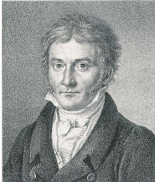
\includegraphics[width=\marginparwidth]{gauss} Friedrich Gauss (1777$-$1855, German) }
Well, what does this have to do with Poisson\rq s equation? If we solve the finitedifference version of Poisson\rq s equation (Eq. \eqref{eg:93}) for $V_{j,k}$ , we find
\begin{equation}\label{eq:98}
f(x_{n+1}=e^{-\bar{x}-\delta_{n}} \approx e^{-\bar{x}}-\delta_{n} e^{-\bar{x}}+\cdots
\end{equation}
With the equation in this form we could just iterate over and over by doing the
following.

\begin{itemize}
\item Choose an initial guess for the interior values of $V_{j,k}$ .
\item Use this initial guess to evaluate the right-hand side of Eq. \eqref{eg:98}
\item Replace our initial guess for $V_{j,k}$ by this right-hand side, and then repeat.

\end{itemize}
If all goes well, then after many iterations the left and right sides of this equation will agree and we will have a solution. \\
To see, let\rq s notice that the iteration process indicated by Eq. \eqref{eg:98} can be
written in matrix form as
\begin{equation}\label{eq:99}
V_{n+1}=\mathbf{L} V_{n}+r
\end{equation}
where $L$ is the matrix which, when multiplied into the vector $V_n$, produces the
$V_{j,k}$ part of the right-hand side of Eq. \eqref{eg:98} and $r$ is the part that depends on the
charge density $ \rho_{j,k}$ . (Don\rq t worry about what $L$ actually looks like; we are just
going to apply general matrix theory ideas to it.) As in the exponential-equation
example given above, let $\bar{V}$ be the exact solution vector and let $\delta_n$ be the error
vector at the $n^{th}$ iteration. The iteration process on the error is, then,
\begin{equation}\label{eq:910}
\delta_{n+1}=\mathbf{L} \delta_{n}
\end{equation}
Now think about the eigenvectors and eigenvalues of the matrix $L$. If the matrix is
well-behaved enough that its eigenvectors span the full solution vector space of
size $N_x × N_y$ , then we can represent $\delta n$ as a linear combination of these eigenvectors. This then invites us to think about what iteration does to each eigenvector. The answer, of course, is that it just multiplies each eigenvector by its eigenvalue.
Hence, for iteration to work we need all of the eigenvalues of the matrix $L$ to have
magnitudes less than 1.\\
So we can now restate the conditions for this approach to work: Iteration on
Eq. \eqref{eg:98} converges if all of the eigenvalues of the matrix $L$ on the right-hand side
of Eq. \eqref{eg:98} are less than 1 in magnitude. This statement is a theorem which can be
proved if you are really good at linear algebra, and the entire iteration procedure
described by Eq. (9.9) is known as Jacobi iteration. Unfortunately, even though
all of the eigenvalues have magnitudes less than 1 there are lots of them that have
magnitudes very close to 1, so the iteration takes forever to converge (the error
only goes down by a tiny amount each iteration). \\ 
But Gauss and Seidel discovered that the process can be accelerated by making
a very simple change in the process. Instead of only using old values of $V_{j,k}$ on
the right-hand side of Eq. \eqref{eg:98}, they used values of $V_{j,k}$ as they became available
during the iteration. (This means that the right side of \eqref{eg:98} contains a mixture
of $V$ -values at the $n$ and $n +1$ iteration levels.) This change, which is called GaussSeidel iteration is really simple to code; you just have a single array in which to
store $V_{j,k}$ and you use new values as they become available. Here as a coded
example of Guass-Seidel iteration for a rectangular region grounded on two sides,
with the two other sides held at a potential:
\begin{lstlisting}
from mpl_toolkits.mplot3d import Axes3D
import matplotlib.pyplot as plt
import numpy as np

# Make the grid
xmin = 0
xmax = 2
Nx = 80
x,hx = np.linspace(xmin,xmax,Nx,retstep = True)
hx2 = hx**2

ymin = 0
ymax = 2
Ny = 40
y,hy = np.linspace(ymin,ymax,Ny,retstep = True)
hy2 = hy**2
X,Y = np.meshgrid(x,y,indexing='ij')

# Initialize potential
V = 0.5*np.ones_like(X)

# Enforce boundary conditions
V[:,0] = 0

V[:,-1] = 0
V[0,:] = 1
V[-1,:] = 1

# Allow possibility of charge distribution
rho = np.zeros_like(X)

# Iterate
denom = 2/hx2 + 2/hy2
fig = plt.figure(1)
for n in range(200):
	# make plots every few steps
	if n % 10 == 0:
		plt.clf()
		ax = fig.gca(projection='3d')
		surf = ax.plot_surface(X,Y,V)
		ax.set_zlim(-0.1, 2)
		plt.xlabel('x')
		plt.ylabel('y')
		plt.draw()
		plt.pause(0.1)

	# Iterate the solution
	for j in range(1,Nx-1):
		for k in range(1,Ny-1):
			V[j,k] = ( (V[j+1,k] + V[j-1,k])/hx2
				+(V[j,k+1] + V[j,k-1])/hy2
				+rho[j,k]) / denom
\end{lstlisting}
\paragraph*{P9.2}  Paste the code above into a program, run it, and watch the solution iterate.
Study the code, especially the part in the loop. When you understand the
code, call a TA over and explain it to them to pass off this part.


\section*{Successive over-relaxation}
\addcontentsline{toc}{section}{Successive over-relaxation}
Gauss-Seidel iteration is not the best we can do, however. To understand the next
improvement let\rq s go back to the exponential example

\begin{equation}\label{eq:911}
x_{n+1}=e^{-x_{n}}
\end{equation}
and change the iteration procedure in the following non-intuitive way:
\begin{equation}\label{eq:912}
x_{n+1}=\omega e^{-x_{n}}+(1-\omega) x_{n}
\end{equation}
where $\omega$ is a number which is yet to be determined.
\paragraph*{P9.3} Verify quickly on paper that even though Eq. \eqref{eg:912} looks quite different
from Eq. \eqref{eg:911}, it is still solved by $x = e^{-x}$.
If we insert xn = x¯ + δn into this new equation and expand as before, the error
changes as we iterate according to the following
\begin{equation}\label{eq:913}
x_{n+1}=\omega e^{-x_{n}}+(1-\omega) x_{n}
\end{equation}

Notice what would happen if we chose $\omega$ so that the factor in parentheses were
zero: The equation says that we would find the correct answer in just one step! Of
course, to choose $\omega$ this way we would have to know $\bar{x}$, but it is enough to know
that this possibility exists at all. All we have to do then is numerically experiment
with the value of $\omega$ and see if we can improve the convergence.

\paragraph*{P9.4} Write a program that accepts a value of $\omega$ and runs the iteration in Eq. \eqref{eg:912}.
Experiment with various values of $\omega$ until you find one that does the best
job of accelerating the convergence of the iteration. You should find that
the best $\omega$ is near 0.64, but it won’t give convergence in one step. See if you
can figure out why not.\\
Hint: Think about the approximations involved in obtaining Eq. \eqref{eg:913}. Specifically go back to the previous derivation and look for terms represented by dots.\\
As you can see from Eq. \eqref{eg:913}, this modified iteration procedure shifts the
error multiplier to a value that converges better. So now we can see how to
improve Gauss-Seidel: we just use an $\omega$ multiplier like this:
\begin{equation}\label{eq:914}
V_{n+1}=\omega\left(\mathbf{L} V_{n}+r\right)+(1-\omega) V_{n}
\end{equation}
then play with $\omega$ until we achieve almost instantaneous convergence. \\ 
Sadly, this doesn\rq t quite work. The problem is that in solving for $N_x × N_y$
unknown values $V_{j,k}$ we don\rq t have just one multiplier; we have one for each
eigenvalue of the matrix. So if we shift one of the eigenvalues to zero, we might
shift another one to a value with magnitude larger than 1 and the iteration will
not converge at all. The best we can do is choose a value of $\omega$ that centers the
entire range of eigenvalues symmetrically between −1 and 1. \\ 
Using an $\omega$ multiplier to shift the eigenvalues is called Successive OverRelaxation, or SOR for short. Here it is written out so you can code it:
\begin{equation}\label{eq:915}
V_{j, k}=\omega\left(\frac{V_{j+1, k}+V_{j-1, k}}{h_{x}^{2}}+\frac{V_{j, k+1}+V_{j, k-1}}{h_{y}^{2}}+\frac{\rho_{j, k}}{\epsilon_{0}}\right) /\left(\frac{2}{h_{x}^{2}}+\frac{2}{h_{y}^{2}}\right)+(1-\omega) V_{j, k}
\end{equation}
And what value should we use for $\omega$? The answer is that it depends on the values
of $N_x and N_y$ . In all cases ω should be between 1 and 2, with $\omega = 1.7$ being a
typical value. Some wizards of linear algebra have shown that the best value of $\omega$ when the computing region is rectangular and the boundary values of $V$ are fixed (Dirichlet boundary conditions) is given by
\begin{equation}\label{eq:916}
\omega=\frac{2}{1+\sqrt{1-R^{2}}}
\end{equation}
where
\begin{equation}\label{eq:917}
R=\frac{h_{y}^{2} \cos \left(\pi / N_{x}\right)+h_{x}^{2} \cos \left(\pi / N_{y}\right)}{h_{x}^{2}+h_{y}^{2}}
\end{equation}
These formulas usually give a reasonable estimate of the best $\omega$ to use. Note,
however, that this value of $\omega$ was found for the case of a cell-edge grid with the
potential specified at the edges. If you use a cell-centered grid with ghost points,
and especially if you change to derivative boundary conditions, this value of $\omega$
won\rq t be quite right. But there is still a best value of $\omega$ somewhere near the value
given in Eq. \eqref{eg:916} and you can find it by numerical experimentation. \\ 
Finally, we come to the question of when to stop iterating. It is tempting just to watch the values of $V_{j, k}$ and quit when the values stabilize at some level, like this for instance: quit when $\epsilon=\left|V(j, k)_{n+1}-V(j, k)_{n}\right|<10^{-6}$. You will see this error criterion sometimes used in books, but do not use it. We know of one person who published an incorrect result in a journal because this error criterion lied. We done\rq t want to quit when the algorithm has quit changing $V$; we want to quit when Poisson\rq s equation is satisfied. (Most of the time these are the same, but only looking at how $V$ changes is a dangerous habit to acquire.) In addition, we want to use a relative (\%) error criterion. This is easily done by setting a scale voltage $V_{\text {scale }}$ which is on the order of the biggest voltage in the problem and then using for the error criterion

\begin{equation}\label{eq:918}
\epsilon=\left|\frac{\text { Lhs }-\mathrm{Rhs}}{V_{\text {scale }}}\right|
\end{equation}
where Lhs is the left-hand side of Eq. \eqref{eg:98} and Rhs is its right-hand side. Because this equation is just an algebraic rearrangement of our finite-difference approximation to Poisson\rq s equation, $\epsilon$ can only be small when Poisson\rq s equation is satisfied. (Note the use of absolute value; can you explain why it is important to use it? Also note that this error is to be computed at all of the interior grid points. Be sure to find the maximum error on the grid so that you only quit when the solution has converged throughout the grid.)\\

And what value should we choose for the error criterion so that we know when to quit? Well, our finite-difference approximation to the derivatives in Poisson\rq s equation is already in error by a relative amount of about $1 /\left(12 N^{2}\right)$, where $N$ is the smaller of $N_{x}$ and $N_{y}$. There is no point in driving $\epsilon$ below this estimate. For more details, and for other ways of improving the algorithm, see Numerical Recipes, Chapter $19 .$

\paragraph*{P9.5}
Starting with the Gauss-Seidel example above, implement all of the improvements described above to write a full successive over-relaxation routine. Note that you will need to replace the $for$ loop on the variable $n$ into a while loop that is based on the error criterion. Also move the plot command out of the loop so it only executes once, after the solution has converged. (So that you don\rq t have to wait for a bunch of plots to be drawn.) Run your code for a spatial region of size $L_{x}=4$ in the x-dimension and $L_{y}=2$ the $\mathrm{y}$-dimension arranged as shown in Fig. 9.1. Use $\mathrm{Nx}=\mathrm{Ny}=30$ and several different values of $\omega$. Note that the boundary conditions on the potential $V(x, y)$ are $V\left(-L_{x} / 2, y\right)=V\left(L_{x} / 2, y\right)=1$ and $V(x, 0)=V\left(x, L_{y}\right)=0$. Set the error criterion to $10^{-4}$. Verify that the optimum value of $\omega$ given by Eq. \eqref{eg:916} is the best one to use.


	\marginpar{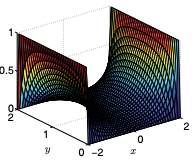
\includegraphics[width=\marginparwidth]{fig91}\captionof{figure}{The electrostatic potential $V(x, y)$ with two sides grounded and two sides at constant potential.}}
\section*{Some Different Geometries}
\addcontentsline{toc}{section}{Some Different Geometries}
\paragraph*{P9.6}
	\marginpar{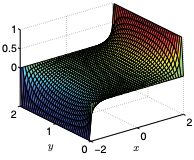
\includegraphics[width=\marginparwidth]{fig92}\captionof{figure}{The potential $V(x, y)$ rom Problem 9.6(a).}}
		\marginpar{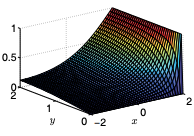
\includegraphics[width=\marginparwidth]{fig93}\captionof{figure}{The potential $V(x, y)$ with zero-derivative boundary conditions on two sides (Problem 9.6(b).)}}
\begin{enumerate}[label=(\alph*)]
\item Modify your code to model a rectangular pipe with $V(x=-2, y)=-1$, $V(x=2, y)=1$, and the $y=0$ and $y=L_{y}$ edges held at $V=0$.
\item Modify your code from (a) so that the boundary condition at the $x=$ $-L_{x} / 2$ edge of the computation region is $\partial V / \partial x=0$ and the boundary condition on the $y=L_{y}$ edge is $\partial V / \partial y=0$. You can do this problem either by changing your grid and using ghost points or by using a quadratic extrapolation technique (see Eq. \eqref{eg:210}). Both methods work fine, but note that you will need to enforce boundary conditions inside the main SOR loop now instead of just setting the values at the edges and then leaving them alone.
You may discover that the script runs slower on this problem. See if you can make it run a little faster by experimenting with the value of $\omega$ that you use. Again, changing the boundary conditions can change the eigenvalues of the operator. (Remember that Eq. (9.16) only works for cell-edge grids with fixed-value boundary conditions, so it only gives a ballpark suggestion for this problem.)
\item Study electrostatic shielding by going back to the boundary conditions of Problem 9.6(a), while grounding some points in the interior of the full computation region to build an approximation to a grounded cage. Allow some holes in your cage so you can see how fields leak in. First make a rectangular cage similar to Fig. 9.4, but then you can try other geometries.
You will need to be creative about how you build your cage and about how you make SOR leave your cage points grounded as it iterates. One thing that won\rq t work is to let SOR change all the potentials, then set the cage points back to $V=0$ before doing the next iteration. This takes forever to converge. It is much better to set them to zero and force SOR to never change them. An easy way to do this is to use a cell-edge grid with a mask. A mask is an array that you build that is the same size as $V$, initially defined to be full of ones like this
\begin{lstlisting}
mask = np.ones_like(V)
\end{lstlisting}
Then you go through and set the elements of mask that you don't want SOR to change to have a value of zero. (We'll let you figure out the logic to do this for the cage.) Once you have your mask built, you add an if statement to our code so that the SOR stuff inside the $j$ and $k$ for loops only changes a given point and updates the error if $\operatorname{mask}(j, k)$ is one. This logic assumes you have to set the values of $V$ for these points before the for loop execute, just like the boundary conditions. Using this technique you can calculate the potential for quite complicated shapes just by changing the mask array.
\includegraphics[width=0.7\textwidth]{fig94}\captionof{figure}{The potential $V (x, y)$ for an electrostatic \rq\rq cage\lq\lq formed by
grounding some interior points. (Problem 9.6(c).)}
\end{enumerate}


\chapter*{The Continuity Equation}
\addcontentsline{toc}{chapter}{The Continuity Equation}
So far we have studied the numerical solution of partial differential equations one at a time, but in many interesting situations the problem to be solved involves coupled systems of differential equations. A "simple" example of such a system are the three coupled one-dimensional equations of gas dynamics. These are the equations of acoustics in a long tube with mass density $\rho(x, t)$, pressure $p(x, t)$, and gas velocity $v(x, t)$ as the dynamic variables. In the next lab we will tackle the hard problem of simultaneously advancing $\rho, T$, and $v$ in time and space, which will require three equations. But for now we will just practice on the continuity equation to develop the tools we need to do the full problem.
\section*{The Continuity Equation}
\addcontentsline{toc}{section}{The Continuity Equation}
The equation that enforces conservation of mass in acoustics is called the continuity equation:
\begin{equation}\label{eq:101}
\epsilon=\left|\frac{\text { Lhs }-\mathrm{Rhs}}{V_{\text {scale }}}\right|
\end{equation}
This equation says that as the gas particles are moved by the flow velocity $v(x, t)$, the density $\rho(x, t)$ is carried along with the flow and can be compressed or rarefied, but mass is not created or destroyed in this process.

Boundary conditions for the continuity equation are a bit different than we\rq ve encountered to this point. This is a convection equation, meaning that if you stand at a point in the flow, the solution at your location arrives (is convected to you) from further \rq\rq upwind.\lq\lq This has a strong effect on the boundary conditions. Suppose, for instance, that the flow field $v(x)$ is always positive, meaning that the wind is blowing to the right. At the left-hand boundary it makes sense to specify $\rho$ because somehow you might arrange to feed density in at that point so that it can be convected across the grid. But at the right boundary it makes no sense at all to specify a boundary condition because when the solution arrives there we just want to let the wind blow it away. (An exception to this rule occurs if $v=0$ at the boundary. In this case there is no wind to blow the solution from anywhere and it would be appropriate to specify a boundary condition.) We\rq ll try several approaches to represent these boundary conditions.

\paragraph*{P10.1}
Let\rq s start with something really simple and inaccurate just to see what can
go wrong. If we use a nicely centered difference in $x$ and an inaccurate
forward difference in $t$, we find
\begin{equation}\label{eq:102}
\frac{\rho_{j}^{n+1}-\rho_{j}^{n}}{\tau}+\frac{1}{2 h}\left(\rho_{j+1}^{n} v_{j+1}-\rho_{j-1}^{n} v_{j-1}\right)=0
\end{equation}
Solve this equation for $\rho_{j}^{n+1}$ and use it in a time-advancing script like the one you built to do the wave equation in Lab 5. Use a cell-center grid with ghost points (use about 400 grid points). For initial conditions use
\begin{equation}\label{eq:103}
\rho(x, 0)=1+e^{-200(x / L-1 / 2)^{2}}
\end{equation}
with $ x \in[0, L], L=10$ , and


\begin{equation}\label{eq:104}
v(x)=v_0
\end{equation}
with $v_{0}=1$. At the left end use $\rho(0, t)=1$ and at the right end try the following two things:
\begin{enumerate}[label=(\roman*)]
\item Set a boundary condition: $\rho(L, t)=1$.
\item Just let mass leave by using linear extrapolation:
	\begin{equation}\label{eq:105}
\rho(L, t)=2 \rho(L-h, t)-\rho(L-2 h, t) \quad \text { or } \quad \rho_{N+1}=2 \rho_{N}-\rho_{N-1}
\end{equation}


\end{enumerate}
Run this algorithm with these two boundary conditions enough times, and with small enough time steps, that you become convinced that $\rho(L, t)=1$ is wrong and that the entire algorithm is worthless because it is unstable.\\
As you might guess from the previous problem, the diffusion equation's simple appearance can be deceiving; it is one of the most difficult equations to solve numerically in all of computational physics because stable methods tend to be inaccurate and accurate methods tend either to be unstable, or non-conservative (as time runs mass spontaneously disappears), or unphysical (mass density and/or pressure become negative.)\\
Let\rq s try another method, known as the Lax-Wendroff method. The idea of the Lax-Wendroff algorithm is to use a Taylor series in time to obtain a second-order accurate method. Taylor expanding the density function in time gives us
\begin{equation}\label{eq:106}
\rho(x, t+\tau)=\rho(x, t)+\tau \frac{\partial \rho}{\partial t}+\frac{\tau^{2}}{2} \frac{\partial^{2} \rho}{\partial t^{2}}
\end{equation}
We can write the continuity equation as
\begin{equation}\label{eq:107}
\frac{\partial \rho}{\partial t}=-\frac{\partial}{\partial x}(\rho v)
\end{equation}
Substituting into our Taylor expansion then gives
\begin{equation}\label{eq:108}
\rho(x, t+\tau)=\rho(x, t)-\tau \frac{\partial}{\partial x}(\rho v)+\frac{\tau^{2}}{2} \frac{\partial}{\partial t}\left(-\frac{\partial}{\partial x}(\rho v)\right)
\end{equation}
If we reverse the order of the derivatives in the last term and assume that $v$ is not
a function of time, we can use Eq. \eqref{eg:107} again to obtain.
\begin{equation}\label{eq:109}
\rho(x, t+\tau)=\rho(x, t)-\tau \frac{\partial \rho v}{\partial x}+\frac{\tau^{2}}{2} \frac{\partial}{\partial x}\left(v \frac{\partial \rho v}{\partial x}\right)
\end{equation}
Finally, we subtract $ρ(x,t)$ from both sides and divide by $\tau$ to obtain
\begin{equation}\label{eq:1010}
\frac{\rho(x, t+\tau)-\rho(x, t)}{\tau}=-\frac{\partial \rho v}{\partial x}+\frac{\tau}{2} \frac{\partial}{\partial x}\left(v \frac{\partial \rho v}{\partial x}\right)
\end{equation}
If we interpret the left-hand side as a time derivative, the second term on the right looks essentially like the diffusion equation. Since the equation we are solving is pure convection, the appearance of diffusion is not good news, but at least this algorithm is better than the horrible one in 10.1. Notice also that the diffusion coefficient in Eq. \eqref{eg:101} is proportional to $\tau$ (stare at it until you can see that this is true), so if small time steps are being used diffusion won't hurt us too much.

\paragraph*{P10.2}
 Finite difference the expression in Eq. \eqref{eq:1010} assuming that $v(x) = v0 =
const$, to find the Lax-Wendroff algorithm:
\begin{equation}\label{eq:1011}
\rho_{j}^{n+1}=\rho_{j}^{n}-\frac{v_{0} \tau}{2 h}\left(\rho_{j+1}^{n}-\rho_{j-1}^{n}\right)+\frac{v_{0}^{2} \tau^{2}}{2 h^{2}}\left(\rho_{j+1}^{n}-2 \rho_{j}^{n}+\rho_{j-1}^{n}\right)
\end{equation}
Change your script from $10.1$ to use the Lax-Wendroff algorithm. Again, use a cell-center grid with ghost points and about 400 grid points. Also use the same initial condition as in Problem $10.1$ and use the extrapolated boundary condition that just lets the pulse leave.\\
Show that Lax-Wendroff works pretty well unless the time step exceeds a Courant condition. Also show that it has the problem that the peak density slowly decreases as the density bump moves across the grid. (To see this use a relatively coarse grid and a time step just below the stability constraint.\\
Warning: do not run with $\tau=h / v_{0}$. If you do you will conclude that this algorithm is perfect, which is only true for this one choice of time step.) This problem is caused by the diffusive term in the algorithm, but since this diffusive term is the reason that this algorithm is not unstable like the one in 10.1, we suppose we should be grateful.

\section*{Crank-Nicolson Again}
\addcontentsline{toc}{section}{Crank-Nicolson Again}
\marginpar{\includegraphics[width=\marginparwidth]{lax} \\ Peter Lax (b. 1926, American) Lax was the PhD advisor for Burton Wendroff.}

Finally, let\rq s try an implicit method, Crank-Nicolson in fact. As a reminder, the
continuity equation is
\begin{equation}\label{eq:1012}
\frac{\partial \rho}{\partial t}+\frac{\partial}{\partial x}(\rho v)=0
\end{equation}
We can\rq t solve this equation directly because it has two unknowns ( $\rho$ and $v$ ). But if we assume that $v$ is known, then it is possible to solve the equation using CrankNicolson. As usual for Crank-Nicolson, we forward difference in time and center difference in space to find
\begin{equation}\label{eq:1013}
\frac{\rho_{j}^{n+1}-\rho_{j}^{n}}{\tau}=-\frac{v_{j+1}^{n} \rho_{j+1}^{n}-v_{j-1}^{n} \rho_{j-1}^{n}}{2 h}
\end{equation}
Then we use time averaging to put the right side of the equation at the same time
level as the left (i.e. at the $n + 1/2$ time level):
\begin{equation}\label{eq:1014}
\rho_{j}^{n+1}-\rho_{j}^{n}=C_{1}\left(\rho_{j+1}^{n}+\rho_{j+1}^{n+1}\right)-C_{2}\left(\rho_{j-1}^{n}+\rho_{j-1}^{n+1}\right)
\end{equation}
where 
\begin{equation}\label{eq:1015}
C_{1}=-\frac{\tau}{8 h}\left(v_{j+1}^{n}+v_{j+1}^{n+1}\right)
\end{equation}
\begin{equation}\label{eq:1016}
C_{2}=-\frac{\tau}{8 h}\left(v_{j-1}^{n}+v_{j-1}^{n+1}\right)
\end{equation}
Then we put the $\rho^{n+1}$ terms on the left and the $\rho^n$ terms on the right:
\begin{equation}\label{eq:1017}
C_{2} \rho_{j-1}^{n+1}+\rho_{j}^{n+1}-C_{1} \rho_{j+1}^{n+1}=-C_{2} \rho_{j-1}^{n}+\rho_{j}^{n}+C_{1} \rho_{j+1}^{n}
\end{equation}
Then we write these equations along with the boundary conditions in matrix form
\begin{equation}\label{eq:1018}
\mathbf{A} \rho^{n+1}=\mathbf{B} \rho^{n}
\end{equation}
which we solve using linear algebra techniques. For this algorithm to calculate $\rho^{n+1}$, we need to feed it values for $\rho^{n}, v^{n}$, and $v^{n+1}$. For now, let\rq s side-step this issue by assuming that $v(x, t)$ is known, and a constant in time. In the next lab we\rq ll worry about advancing the velocity solution in parallel with the density.
\paragraph*{P10.3}

	\marginpar{\includegraphics[width=\marginparwidth]{fig1001}\captionof{figure}{A pulse is convected across a region in which the convection velocity $v(x)$ is constant (Problem 10.3(b)).}}
	\marginpar{\includegraphics[width=\marginparwidth]{fig1002}\captionof{figure}{A pulse is convected across a region in which the convection velocity $v(x)$ is decreasing. Note that the pulse narrows and grows, conserving mass. (Prob$\operatorname{lem} 10.3(\mathrm{c}))$}}
\begin{enumerate}[label=(\alph*)]
\item  Write a program that implements this algorithm, perhaps starting from one of your programs from the Schr{\"o}dinger equation lab. Work out how to implement the boundary conditions, $\rho(0, t)=1$ and $\rho(L, t)$ is just allowed to leave, by properly defining the top and bottom rows of the matrices $\mathbf{A}$ and $\mathbf{B}$. This involves multiplying $\mathbf{B} \rho^{n}$ to find an $r$-vector as you have done before.
\item  Implement this algorithm with a constant convection velocity $v=$ $v_{0}$ and show that the algorithm conserves amplitude to very high precision and does not widen due to diffusion. These two properties make this algorithm a good one as long as shock waves don\rq t develop.
\item Now use a convection velocity that varies with $x$ :
\begin{equation}\label{eq:1019}
v(x)=1.2-x / L
\end{equation}
This velocity slows down as the flow moves to the right, which means
that the gas in the back is moving faster than the gas in the front,
causing compression and an increase in density. You should see the
slowing down of the pulse and the increase in density in your numerical solution.
\item Go back to a constant convection velocity $v = v_0$ and explore the way
this algorithm behaves when we have a shock wave (discontinuous
density) by using as the initial condition
\begin{equation}\label{eq:1020}
\rho(x, 0)= \begin{cases}1.0 & \text { if } 0 \leq x \leq L / 2 \\ 0 & \text { otherwise }\end{cases}
\end{equation}
The true solution of this problem just convects the step to the right;
you will find that Crank-Nicolson fails at this seemingly simple task.
\item For comparison, try the same step-function initial condition in your
Lax-Wendroff script from Problem 10.2.
\end{enumerate}
Our Crank-Nicolson algorithm is both stable and conservative, but it only
works well if the solution doesn\rq t become too steep. This is a severe limitation,
since we are talking about gas dynamics here and shock waves routinely show up
as solutions in gas dynamics. Numerical methods that properly handle shocks
are much more involved than the ones we will show you here.

\chapter*{One Dimensional Gas Dynamics}
\addcontentsline{toc}{chapter}{One Dimensional Gas Dynamics}
\section*{Simultaneously advancing $\rho$, $T$ , and $v$}
\addcontentsline{toc}{section}{Simultaneously advancing $\rho$, $T$ , and $v$}
Now we are going to use the implicit algorithm that we developed in the previous
lab as a tool to solve the three nonlinear coupled partial differential equations
of one-dimensional gas dynamics. These are the equations of one-dimensional
sound waves in a long tube pointed in the x-direction, assuming that the tube is
wide enough that friction with the walls doesn\rq t matter. \\ 
The three equations we need to advance are the continuity equation
\begin{equation}\label{eq:1101}
\frac{\partial \rho}{\partial t}+\frac{\partial}{\partial x}(\rho v)=0
\end{equation}
the conservation of energy
\begin{equation}\label{eq:1102}
\frac{\partial T}{\partial t}+v \frac{\partial T}{\partial x}+(\gamma-1) T \frac{\partial v}{\partial x}=\frac{(\gamma-1) M \kappa}{k_{B}} \frac{1}{\rho} \frac{\partial^{2} T}{\partial x^{2}}
\end{equation}
and Newton\rq s second law
\begin{equation}\label{eq:1103}
\frac{\partial v}{\partial t}+v \frac{\partial v}{\partial x}=-\frac{1}{\rho} \frac{\partial P}{\partial x}+\frac{4 \mu}{3 \rho} \frac{\partial^{2} v}{\partial x^{2}}
\end{equation}
Here $\rho(x,t)$ is the density of the gas, $v(x,t)$ is the velocity of the gas, and $T(x,t)$ is
the temperature of the gas. The pressure $P$ is given by the ideal gas law
\begin{equation}\label{eq:1104}
P=\frac{k_{B}}{M} \rho T
\end{equation}
Because of the nonlinearity of these equations and the fact that they are
coupled we are not going to be able to write down a simple algorithm that will advance $\rho, T$ , and $v$ in time. But if we are creative we can combine simple methods
that work for each equation separately into a stable and accurate algorithm for
the entire set. We are going to show you one way to do it, but the computational
physics literature is full of other ways, including methods that handle shock waves.
This is still a very active and evolving area of research, especially for problems in
2 and 3 dimensions.
Let\rq s try a predictor-corrector approach similar to second-order Runge-Kutta (which you learned about back in 330 ) by first taking an approximate step in time of length $\tau$ to obtain predicted values for our variables one time step in the future. We'll refer to these first-order predictions for the future values as $\tilde{\rho}^{n+1}, \tilde{T}^{n+1}$, and $\tilde{v}^{n+1}$. In the predictor step we will treat $v$ as constant in time in Eq. \eqref{eq:1101} to predict $\tilde{\rho}^{n+1}$. Then we'll use $\tilde{\rho}^{n+1}$ to help us calculate $\tilde{T}^{n+1}$ using Eq. \eqref{eq:1102}, while still treating $v$ as fixed in time. Once these predicted values are obtained we can use them with Eq. \eqref{eq:1103} to obtain a predicted $\tilde{v}$. With all of these predicted future values of our variables in hand, we do another round of Crank-Nicolson on all three equations to step the solution forward in time. We can represent this procedure schematically as follows:\\
Step 1 Use the old velocity $v^{n}$ as input for Eqn. \eqref{eq:1105} $\rightarrow$ Solve for the predicted density $\tilde{\rho}$.\\
Step 2 Use $v^{n}$ and $\tilde{\rho}$ as inputs for Eqn. \eqref{eq:1102} $\rightarrow$ Solve for the predicted temperature $\tilde{T}$.\\
Step 3 Use $\tilde{\rho}$ and $\tilde{T}$ as inputs for Eqn. \eqref{eq:1103} $\rightarrow$ Solve for the predicted velocity $\tilde{v}$.\\
Step 4 Use $\tilde{v}$ as input for Eqn. \eqref{eq:1105} $\rightarrow$ Solve for the new density $\rho^{n+1}$.\\
Step 5 Use $\tilde{v}$ and $\rho^{n+1}$ as inputs for Eqn. \eqref{eq:1102} $\rightarrow$ Solve for the new temperature $T^{n+1}$.\\
Step 6 Use $\rho^{n+1}$ and $T^{n+1}$ as inputs for Eqn. \eqref{eq:1103} $\rightarrow$ Solve for the new velocity $v^{n+1}$.\\

This procedure probably seems a bit nebulous at this point, so let\rq s go through it in more detail. First we\rq ll derive the Crank-Nicolson algorithms for our three equations, then we\rq ll show how to use these algorithms to solve the system using the predictor-corrector method.


\section*{Continuity Equation}
\addcontentsline{toc}{section}{Continuity Equation}
Conservation of mass is governed by the continuity equation
\begin{equation}\label{eq:1105}
\frac{\partial \rho}{\partial t}+\frac{\partial}{\partial x}(\rho v)=0
\end{equation}

We can\rq t solve this equation directly because it has two unknowns ( $\rho$ and $v$ ). But if we assume that $v$ is known as we did in the last lab, then it is possible to solve the equation using Crank-Nicolson, as we did in the last lab. As usual for Crank-Nicolson, we forward difference in time and center difference in space to find
\begin{equation}\label{eq:1106}
\frac{\rho_{j}^{n+1}-\rho_{j}^{n}}{\tau}=-\frac{v_{j+1}^{n} \rho_{j+1}^{n}-v_{j-1}^{n} \rho_{j-1}^{n}}{2 h}
\end{equation}
Then we use time averaging to put the right side of the equation at the same time level as the left (i.e. at the $n+1 / 2$ time level):

\begin{equation}\label{eq:1107}
\rho_{j}^{n+1}-\rho_{j}^{n}=C_{1}\left(\rho_{j+1}^{n}+\rho_{j+1}^{n+1}\right)-C_{2}\left(\rho_{j-1}^{n}+\rho_{j-1}^{n+1}\right)
\end{equation}
where
\begin{equation}\label{eq:1108}
C_{1}=-\frac{\tau}{8 h}\left(v_{j+1}^{n}+v_{j+1}^{n+1}\right)
\end{equation}
\begin{equation}\label{eq:1109}
C_{2}=-\frac{\tau}{8 h}\left(v_{j-1}^{n}+v_{j-1}^{n+1}\right)
\end{equation}
 Then we put the  $\rho^{n+1}$  terms on the left and the $\rho^{n}$ terms on the right: 

\begin{equation}\label{eq:1110}
C_{2} \rho_{j-1}^{n+1}+\rho_{j}^{n+1}-C_{1} \rho_{j+1}^{n+1}=-C_{2} \rho_{j-1}^{n}+\rho_{j}^{n}+C_{1} \rho_{j+1}^{n}
\end{equation}
Then we write these equations along with the boundary conditions in matrix form

\begin{equation}\label{eq:1111}
\mathbf{A} \rho^{n+1}=\mathbf{B} \rho^{n}
\end{equation}
which we solve using linear algebra techniques. For the algorithm represented by Eq. \eqref{eg:1111} to calculate $\rho^{n+1}$, we need to feed it values for $\rho^{n}, v^{n}$, and $v^{n+1}$. Since the inputs for these variables will be different in the predictor and the corrector steps, we need to invent some notation. We\rq ll refer to this Crank-Nicolson algorithm for stepping forward to find $\rho^{n+1}$ using the notation $S_{\rho}\left(\rho^{n}, v^{n}, v^{n+1}\right)$ so the variables the algorithm needs as inputs are explicitly shown.

\section*{Conservation of energy}
\addcontentsline{toc}{section}{Conservation of energy}

The temperature of a gas is a macroscopic manifestation of the energy of the
thermal motions of the gas molecules. The equation that enforces conservation
of energy for our system is

\begin{equation}\label{eq:1112}
\frac{\partial T}{\partial t}+v \frac{\partial T}{\partial x}=-(\gamma-1) T \frac{\partial v}{\partial x}+D_{T} \frac{\partial^{2} T}{\partial x^{2}}
\end{equation}
where $\gamma$ is the ratio of specific heats in the gas: $\gamma=C_{p} / C_{\nu}$. This equation says that as the gas is moved along with the flow and squeezed or stretched, the energy is convected along with the flow and the pressure goes up and down adiabatically (that\rq s why $\gamma$ is in there). It also says that thermal energy diffuses due to thermal conduction. Thermal diffusion is governed by the diffusion-like term containing the thermal diffusion coefficient $D_{T}$ given in a gas by
\begin{equation}\label{eq:1113}
D_{T}=\frac{(\gamma-1) M \kappa}{k_{B} \rho}
\end{equation}
where $\kappa$ is the thermal conductivity, $M$ is the mass of a molecule of the gas, and where $k_{B}$ is Boltzmann\rq s constant.\\
It is probably easier to conceptualize pressure waves rather than temperature waves. The ideal gas law gives us a way to calculate the pressure, given a density $\rho$ and a temperature $T$, so we\rq ll use the ideal gas law $P=n k_{B} T$ (where $n$ is the number of particles per unit volume) to calculate pressure $P$ once the density $\rho$ and temperature $T$ are known via
\begin{equation}\label{eq:1114}
P=\frac{k_{B}}{M} \rho T
\end{equation}
To find a predicted value for T one step in the future, we forward difference
the time derivative and center difference the space derivatives to find

\begin{equation}\label{eq:1115}
\frac{T_{j}^{n+1}-T_{j}^{n}}{\tau}=-v_{j}^{n} \frac{T_{j+1}^{n}-T_{j-1}^{n}}{2 h}-(\gamma-1) T_{j}^{n} \frac{v_{j+1}^{n}-v_{j-1}^{n}}{2 h}+F \frac{1}{\rho_{j}^{n}} \frac{T_{j+1}^{n}-2 T_{j}^{n}+T_{j-1}^{n}}{h^{2}}
\end{equation}
where
\begin{equation}\label{eq:1116}
F=\frac{(\gamma-1) M \kappa}{k_{B}}
\end{equation}
We then rearrange Eq. \eqref{eg:1115} into a form that makes the upcoming algebra (and
coding) more readable:
\begin{equation}\label{eq:1117}
\frac{T_{j}^{n+1}-T_{j}^{n}}{\tau}=T_{j-1}^{n} D_{1}+T_{j}^{n} D_{2}+T_{j+1}^{n} D_{3}
\end{equation}
where
\begin{equation}\label{eq:1118}
D_{1}=\frac{v_{j}^{n}}{2 h}+\frac{F}{\rho_{j}^{n} h^{2}}
\end{equation}

\begin{equation}\label{eq:1119}
D_{2}=-(\gamma-1) \frac{v_{j+1}^{n}-v_{j-1}^{n}}{2 h}-\frac{2 F}{\rho_{j}^{n} h^{2}}
\end{equation}
\begin{equation}\label{eq:1120}
D_{3}=-\frac{v_{j}^{n}}{2 h}+\frac{F}{\rho_{j}^{n} h^{2}}
\end{equation}
\paragraph*{P11.1}
Finish deriving the Crank-Nicolson algorithm for $T^{n+1}$ by putting the righthand side of Eq. \eqref{eg:1117} at the $n+1 / 2$ time level. This means replacing $T^{n}$ terms with $\left(T^{n}+T^{n+1}\right) / 2$ in Eq. \eqref{eg:1117} and making the replacements $\rho^{n} \Rightarrow\left(\rho^{n}+\rho^{n+1}\right) / 2$ and $v^{n} \Rightarrow\left(v^{n}+v^{n+1}\right) / 2$ in $D_{1}, D_{2}$, and $D_{3}$. Then put your system of equations in the form
\begin{equation*}
\mathbf{A} T^{n+1}=\mathbf{B} T^{n}
\end{equation*}
and write out the coefficients in the $\mathbf{A}$ and $\mathbf{B}$ matrices so we can code them later.
When you are finished with Problem $11.1$ you will have an algorithm for stepping $T$ forward in time. We'll refer to this algorithm as $S_{T}\left(T^{n}, v^{n}, v^{n+1}, \rho^{n}, \rho^{n+1}\right)$, so we explicitly see the variables that are required as inputs.
\section*{Newton\rq s second law}
\addcontentsline{toc}{section}{Newton\rq s second law}
Finally, let\rq s consider Newton\rq s second law for this system in a form analogous to $a=F / m$ :

\begin{equation}\label{eq:1121}
\frac{\partial v}{\partial t}+v \frac{\partial v}{\partial x}=-\frac{1}{\rho} \frac{\partial P}{\partial x}+\frac{4 \mu}{3 \rho} \frac{\partial^{2} v}{\partial x^{2}}
\end{equation}
You should recognize the first term $d \nu / d t$ as acceleration, and we\rq ll discuss the origin of the other acceleration term in a minute. The first term on the right is the pressure force that pushes fluid from high pressure toward low pressure, with the pressure $P$ given by the ideal gas law in Eq. \eqref{eq:1114}. The second term on the right represents the force of internal friction called viscosity, and the parameter $\mu$ is referred to as the coefficient of viscosity. (Tar has high viscosity, water has medium viscosity, and air has almost none.) The $1 / \rho$ factor in the force terms represents the mass $m$ in $a=F / m$ (but of course we are working with mass density $\rho$ here).
You may be unconvinced that the left side of Eq. \eqref{eq:1121} is acceleration. To become more convinced, let\rq s think about this situation more carefully. Newton\rq s second law does not apply directly to a location in space where there is a moving fluid. Newton\rq s second law is for particles that are moving through space, not for a location in space that is sitting still with fluid moving through it. This distinction is subtle, but important. Think, for instance, about a steady stream of honey falling out of a honey bear held over a warm piece of toast. If you followed a piece of honey along its journey from the spout down to the bread you would experience acceleration. But if you watched a piece of the stream at a specific location (say, $10 \mathrm{~cm}$ above the bread) you would see that the velocity of this part of the stream is constant in time: $\partial v / \partial t=0$. This is a strong hint that there is more to describing the acceleration of fluids through a region of space than just the local $\partial v / \partial t$ for a given location. You also need to compare the local velocity at your chosen point to the velocities at nearby points in space, which is what the $v \partial v / \partial x$ term does in the left side of Eq. \eqref{eq:1121}.
Notice that Eq. \eqref{eg:1121} has a nonlinear term on the left: $v(\partial v / \partial x)$. There is no way to directly represent this nonlinear term using a linear matrix form like $\mathbf{A} v^{n+1}=\mathbf{B} v^{n}$, so we'll have to make an approximation. We\rq ll assume that the leading $v$ in the nonlinear term is somehow known and designate it as $\bar{v}$. (We\rq ll deal with finding something to use for $\bar{\nu}$ later.) With a forward time derivative and a centered space derivative, we have


\begin{equation}\label{eq:1122}
\begin{array}{r}
\frac{v_{j}^{n+1}-v_{j}^{n}}{\tau}=-\bar{v}_{j}^{n}\left(\frac{v_{j+1}^{n}-v_{j-1}^{n}}{2 h}\right)-\frac{k_{B}}{M \rho_{j}^{n}}\left(\frac{\rho_{j+1}^{n} T_{j+1}^{n}-\rho_{j-1}^{n} T_{j-1}^{n}}{2 h}\right) \\
+\frac{4 \mu}{3 \rho_{j}^{n}}\left(\frac{v_{j+1}^{n}-2 v_{j}^{n}+v_{j-1}^{n}}{h^{2}}\right)
\end{array}
\end{equation}
Again, we\rq ll rewrite the equations with named groups of expressions that don\rq t
depend on $v$ so that our algebra is manageable:


\begin{equation}\label{eq:1123}
\frac{v_{j}^{n+1}-v_{j}^{n}}{\tau}=E_{0}+v_{j-1}^{n} E_{1}+v_{j}^{n} E_{2}+v_{j+1}^{n} E_{3}
\end{equation}
where

\begin{equation}\label{eq:1124}
E_{0}=-\frac{k_{B}}{M \rho_{j}^{n}}\left(\frac{\rho_{j+1}^{n} T_{j+1}^{n}-\rho_{j-1}^{n} T_{j-1}^{n}}{2 h}\right)
\end{equation}
\begin{equation}\label{eq:1125}
E_{1}=\frac{\bar{v}_{j}^{n}}{2 h}+\frac{4 \mu}{3 \rho_{j}^{n} h^{2}}
\end{equation}

\begin{equation}\label{eq:1126}
E_{2}=-\frac{8 \mu}{3 \rho_{j}^{n} h^{2}}
\end{equation}

\begin{equation}\label{eq:1127}
E_{3}=-\frac{\bar{v}_{j}^{n}}{2 h}+\frac{4 \mu}{3 \rho_{j}^{n} h^{2}}
\end{equation}

\paragraph*{P11.2}
Finish deriving the Crank-Nicolson algorithm for $v$ by making the replacements $v^{n} \Rightarrow\left(v^{n+1}+v^{n}\right) / 2$ the right-hand side of Eq. \eqref{eg:1123} and $\rho^{n} \Rightarrow$ $\left(\rho^{n}+\tilde{\rho}^{n+1}\right) / 2, T^{n} \Rightarrow\left(T^{n}+\tilde{T}^{n+1}\right) / 2$, and $\bar{v}^{n} \Rightarrow\left(\bar{v}^{n}+\bar{v}^{n+1}\right) / 2$ in $E_{0}, E_{1}, E_{2}$, and $E_{3}$. Show that your system of equations needs to be in the form

\begin{equation*}
\mathbf{A} v^{n+1}=\mathbf{B} v^{n}+E_{0}
\end{equation*}
where $E_{0}$ is a column vector. Write out the coefficients in the $\mathbf{A}$ and $\mathbf{B}$ matrices so you can code them later.

We\rq ll refer to this $v$-stepping algorithm as $S_{v}\left(v^{n}, \bar{v}^{n}, \bar{v}^{n+1}, \rho^{n}, \rho^{n+1}, T^{n}, T^{n+1}\right)$, where, as usual, we explicitly show the variables that are required as inputs.
\section*{Waves in a closed tube}
\addcontentsline{toc}{section}{Waves in a closed tube}

Now that you have algorithms for all three equations, we can restate the predictorcorrector algorithm using our newly-developed notation.
Predictor Step: First we predict $\rho^{n+1}$ while treating $v$ as a constant:
$$
\tilde{\rho}^{n+1}=S_{\rho}\left(\rho^{n}, v^{n}, v^{n+1}=v^{n}\right)
$$
Then we predict $T^{n+1}$ using $\tilde{\rho}^{n+1}$, still treating $v$ as a constant
$$
\tilde{T}^{n+1}=S_{T}\left(T^{n}, v^{n}, v^{n+1}=v^{n}, \rho^{n}, \rho^{n+1}=\tilde{\rho}^{n+1}\right)
$$
Then we predict $v^{n+1}$ using $\tilde{\rho}^{n+1}$ and $\tilde{T}^{n+1}$, while treating $\bar{v}$ from the nonlinear term as a constant equal to the current $v$
$$
\tilde{v}^{n+1}=S_{v}\left(v^{n}, \bar{v}^{n}=v^{n}, \bar{v}^{n+1}=v^{n}, \rho^{n}, \rho^{n+1}=\tilde{\rho}^{n+1}, T^{n}, \tilde{T}^{n+1}\right)
$$
Corrector Step: Now that we have predicted values for each variable, we step $\rho$ forward using
$$
\rho^{n+1}=S_{\rho}\left(\rho^{n}, v^{n}, v^{n+1}=\tilde{v}^{n}\right)
$$
Then we step $T$ using
$$
T^{n+1}=S_{T}\left(T^{n}, v^{n}, v^{n+1}=\tilde{v}^{n}, \rho^{n}, \rho^{n+1}\right)
$$
And finally, we step $v$ forward using
$$
v^{n+1}=S_{v}\left(v^{n}, \bar{v}^{n}=v^{n}, \bar{v}^{n+1}=\tilde{v}^{n}, \rho^{n}, \rho^{n+1}, T^{n}, T^{n+1}\right)
$$
Now let\rq s put this algorithm into a script and use it to model waves in a tube of length $L=10 \mathrm{~m}$ with closed ends through which there is no flow of heat. For disturbances in air at sea level at $20^{\circ} \mathrm{C}$ we have temperature $T=293 \mathrm{~K}$, mass density $\rho=1.3 \mathrm{~kg} / \mathrm{m}^{3}$, adiabatic exponent $\gamma=1.4$, coefficient of viscosity $\mu=$ $1.82 \times 10^{-5} \mathrm{~kg} /(\mathrm{m} \cdot \mathrm{s})$, and coefficient of thermal conductivity $\kappa=0.024 \mathrm{~J} /(\mathrm{m} \cdot \mathrm{s} \cdot \mathrm{K})$. Boltzmann\rq s constant is $k_{B}=1.38 \times 10^{-23} \mathrm{~J} / \mathrm{K}$ and the mass of the molecules of the gas is $M=29 \times 1.67 \times 10^{-27} \mathrm{~kg}$ for air.

\paragraph*{P11.3}
\begin{enumerate}[label=(\alph*)]
	\item As you might guess, debugging the algorithm that we just developed takes a while to debug because there are so many steps and so many terms to get typed accurately. (When we wrote the solution code, it took over an hour to track down two minus sign errors and a factor of two error.) We\rq d rather have you use the algorithm than beat your head on the wall debugging it, so below is the code that implements the algorithm. Go to the class web site now and download these files. Study them and make sure you understand how they work.
	\item The one thing we haven\rq t included in the code is the boundary conditions. The ends are insulating, so we have
	\begin{equation}\label{eq:1128}
\partial T / \partial x=0
\end{equation}
at both ends. Because the wall ends are fixed and the gas can\rq t pass through these walls, the boundary conditions on the velocity are
\begin{equation}\label{eq:1129}
v(0, t)=v(L, t)=0
\end{equation}
Use this fact to obtain the following differential boundary condition
on the density at the ends of the tube:

\begin{equation}\label{eq:1130}
\frac{\partial \rho}{\partial t}+\rho \frac{\partial v}{\partial x}=0 \quad \text { at } x=0 \text { and } x=L
\end{equation}
This condition simply says that the density at the ends goes up and
down in obedience to the compression or rarefaction produced by the
divergence of the velocity.
Write down the finite difference form for all three of these boundary
conditions. Make sure they are properly centered in time and space
for a cell-center grid with ghost points. Then code these boundary
conditions in the proper spots in the code.

\end{enumerate}

\paragraph*{P11.4}
\begin{enumerate}[label=(\alph*)]
\item Test the script by making sure that small disturbances travel at the sound speed $c=\sqrt{\frac{\gamma k_{B} T}{M}}$. To do this set $T$ and $\rho$ to their atmospheric values and set the velocity to 
\begin{equation}\label{eq:1131}
\frac{\partial \rho}{\partial t}+\rho \frac{\partial v}{\partial x}=0 \quad \text { at } x=0 \text { and } x=L
\end{equation}
with $v_{0}=c / 100$. If you look carefully at the deviation of the density from its atmospheric value you should see two oppositely propagating signals. Verify that they travel at the speed of sound.

\item The predictor-corrector algorithm is not as stable as plain CrankNicolson. Vary the time step and find where it begins to be unstable. Then change $N$ and see how the stability threshold changes. Come up with an equation that estimates a limit on the step size in terms of $h$.

\item Remove the effects of viscosity and thermal conduction by setting $\mu=0$ and $\kappa=0$. Increase the value of $v_{0}$ to $c / 10$ and beyond and watch how the pulses develop. You should see the wave pulses develop steep leading edges and longer trailing edges; you are watching a shock wave develop. But if you wait long enough you will see your shock wave develop ugly wiggles; these are caused by Crank-Nicolson\rq s failure to properly deal with shock waves.

\item Repeat part (c) with non-zero $\mu$ and $\kappa$ and watch thermal conduction and viscosity widen the shock and prevent wiggles. Try artificially large values of $\mu$ and $\kappa$ as well as their actual atmospheric values.
\end{enumerate}
\begin{lstlisting}
import Lab11Funcs as S
import matplotlib.pyplot as plt
import numpy as np

# System Parameters
L = 10.0 # Length of tube
T0 = 293. # Ambient temperature
rho0 = 1.3 # static density (sea level)

# speed of sound
c = np.sqrt(S.gamma * S.kB * T0 / S.M)

# cell-center grid with ghost points
N = 100
h = L/N
x = np.linspace(-.5*h,L+.5*h,N+2)

# initial distributions
rho = rho0 * np.ones_like(x)
T = T0 * np.ones_like(x)
v = np.exp(-200*(x/L-0.5)**2) * c/100

tau = 1e-4
tfinal = 0.1
t = np.arange(0,tfinal,tau)

skip = 5 #input(' Steps to skip between plots - ')

for n in range(len(t)):

	# Plot the current values before stepping
	if n % skip == 0:
		plt.clf()
		plt.subplot(3,1,1)
		plt.plot(x,rho)
		plt.ylabel('rho')
		plt.ylim(1.28, 1.32)
		plt.title('time={:1.3f}'.format(t[n]))
		plt.subplot(3,1,2)
		plt.plot(x,T)
		plt.ylabel('T')
		plt.ylim(292,294)
		plt.subplot(3,1,3)
		plt.plot(x,v)
		plt.ylabel('v')
		plt.ylim(-4,4)
		plt.xlabel('x')
		plt.pause(0.1)
		
# 1. Predictor step for rho
rhop = S.Srho(rho,v,v,tau,h)

# 2. Predictor step for T
Tp = S.ST(T,v,v,rho,rhop,tau,h)

# 3. Predictor step for v
vp = S.Sv(v,v,v,rho,rhop,T,Tp,tau,h)

# 4. Corrector step for rho
rhop = S.Srho(rho,v,vp,tau,h)

# 5. Corrector step for T
Tp = S.ST(T,v,vp,rho,rhop,tau,h)

# 6. Corrector step for v
v = S.Sv(v,v,vp,rho,rhop,T,Tp,tau,h)

# Now put rho and T at the same time-level as v
rho = rhop
T = Tp
\end{lstlisting}




\begin{lstlisting}
import numpy as np
import scipy.linalg as la

# Physical Constants
gamma = 1.4 # Adiabatic Exponent
kappa = 0.024 # Thermal conductivity
kB = 1.38e-23 # Boltzman Constant
M = 29*1.67e-27 # Mass of air molecule (Average)
mu = 1.82e-5 # Coefficient of viscosity
F = (gamma-1)*M*kappa/kB # a useful constant

def Srho(rho,v,vp,tau,h):
	# Step rho forward in time by using Crank-Nicolson
	# on the continuity equation

	N = len(rho)
	A = np.zeros((N,N))
	B = np.zeros_like(A)

	# Load interior points
	const = -tau/8/h
	for j in range(1,N-1):
		C1 = const * (v[j+1] + vp[j+1])
		C2 = const * (v[j-1] + vp[j-1])
		A[j,j-1] = C2
		A[j,j] = 1
		A[j,j+1] = -C1
		B[j,j-1] = -C2
		B[j,j] = 1
		B[j,j+1] = C1
	# Apply boundary condition
	# Write your code here
	
	# Crank Nicolson solve to step rho in time
	r = B@rho

	return la.solve(A,r)

def ST(T,v,vp,rho,rhop,tau,h):

	N = len(T)
	A = np.zeros((N,N))
	B = np.zeros_like(A)

	# Load interior points
	for j in range(1,N-1):
		D1 = (v[j] + vp[j])/(4*h) + 2*F/(rho[j]+rhop[j])/h**2
		D2 = (-(gamma-1) * (v[j+1] + vp[j+1] - v[j-1] - vp[j-1] )/(4*h)
			- 4*F/(rho[j] + rhop[j])/h**2 )
		D3 = -(v[j] + vp[j])/(4*h) + 2*F/(rho[j]+rhop[j])/h**2
		
		A[j,j-1] = -0.5*D1
		A[j,j] = 1/tau - 0.5*D2
		A[j,j+1] = -0.5*D3
		B[j,j-1] = 0.5*D1
		B[j,j] = 1/tau + 0.5*D2
		B[j,j+1] = 0.5*D3
	# Apply boundary condition
	# Insulating: dt/dx = 0
	
	# Write your code here
	
	# Crank Nicolson solve to step rho in time
	
	r = B@T
	return la.solve(A,r)
	
def Sv(v,vbar,vbarp,rho,rhop,T,Tp,tau,h):
	N = len(rho)
	A = np.zeros((N,N))
	B = np.zeros_like(A)
	E0 = np.zeros_like(v)
	
	# Load interior points
	for j in range(1,N-1):
		E0[j] = (-kB/4/h/M/(rho[j]+rhop[j]) *
			( (rho[j+1] + rhop[j+1]) * (T[j+1] + Tp[j+1])
			- (rho[j-1] + rhop[j-1]) * (T[j-1] + Tp[j-1])) )
		E1 = (vbar[j] + vbarp[j])/(4*h)+8*mu/3/h**2/(rho[j]+rhop[j])
		E2 =-16*mu/3/h**2/(rho[j]+rhop[j])
		E3 =-(vbar[j] + vbarp[j])/(4*h) +8*mu/3/h**2/(rho[j]+rhop[j])
		
		A[j,j-1] = -0.5*E1
		A[j,j] = 1/tau - 0.5*E2
		A[j,j+1] = -0.5*E3
		B[j,j-1] = 0.5*E1
		B[j,j] = 1/tau + 0.5*E2
		B[j,j+1] = 0.5*E3
		
	# Apply boundary condition
	# Fixed: v = 0

	# Write your code here
		
		
	# Crank Nicolson solve to step rho in time
	r = B@v + E0
	return la.solve(A,r)
\end{lstlisting}


\chapter*{Solitons: Korteweg-deVries Equation}
\addcontentsline{toc}{chapter}{Solitons: Korteweg-deVries Equation}
	\marginpar{\includegraphics[width=\marginparwidth]{fig1201}\captionof{figure}{The log flume ride at Lagoon produces a solitary wave (marked by arrows in the frames above). The leading edge of the soliton is where the water begins to spill over the side of the trough.}}
At the Lagoon amusement park in Utah, there is a water ride called the Log Flume. It is a standard, old-fashioned water ride where people sit in a 6-seater boat shaped like a log which slowly travels along a fiberglass trough through some scenery, then is pulled up a ramp to an upper level. The slow ascent is followed by a rapid slide down into the trough below, which splashes the passengers a bit, after which the log slowly makes its way back to the loading area. But you can see something remarkable happen as you wait your turn to ride if you watch what happens to the water in the trough when the log splashes down. A large water wave is pushed ahead of the log, as you might expect. But instead of gradually dying away, as you might think a single pulse should in a dispersive system like surface waves on water, the pulse lives on and on. It rounds the corner ahead of the log that created it, enters the area where logs are waiting to be loaded, pushes each log up and down in turn, then heads out into the scenery beyond, still maintaining its shape.

This odd wave is called a \rq\rq soliton\lq\lq, or \rq\rq "solitary wave\lq\lq, and it is an interesting feature of non-linear dynamics that has been widely studied in the last 30 years, or so. The simplest mathematical equation which produces a soliton is the KortewegdeVries equation
\begin{equation}\label{eq:1201}
\frac{\partial y}{\partial t}+y \frac{\partial y}{\partial x}+\alpha \frac{\partial^{3} y}{\partial x^{3}}=0
\end{equation}
which describes surface waves in shallow water. In the first two terms of this
equation you can see the convective behavior we studied in Lab 10, but the last
term, with its rather odd third derivative, is something new. We will be studying
this equation in this laboratory.

\section*{Numerical solution for the Korteweg-deVries equation}
\addcontentsline{toc}{section}{Numerical solution for the Korteweg-deVries equation}
We will begin our study of the Korteweg-deVries equation by using Crank-Nicolson to finite difference it on a grid so that we can explore its behavior by numerical experimentation. The first step is to define a grid, and since we want to be able to see the waves travel for a long time we will copy the trough at Lagoon and make our computing region be a closed loop. We can do this by choosing an interval from $x=0$ to $x=L$, as usual, but then we will make the system be periodic by declaring that $x=0$ and $x=L$ are actually the same point, as would be the case in a circular trough. We will subdivide this region into $N$ subintervals and let $h=L / N$ and $x_{j}=(j-1) h$, so that the grid is cell-edge. Normally such a cell-edge grid would have $N+1$ points, but ours doesn't because the last point $(j=N)$ is just a repeat of the first point: $x_{N}=x_{0}$, because our system is periodic.\\
We now do the usual Crank-Nicolson differencing, where we evaluate each term in the equation at time level $n+1 / 2$. The last term in Eq. \eqref{eg:1201} has a third derivative, so we\rq ll need a reasonable approximation for the third derivative. Suppose you have function values $f(x-3 h / 2), f(x-h / 2), f(x+h / 2)$, and $f(x+$ $3 h / 2)$. A good way to do this is to write down four Taylor's series up to the fifth derivative for the function at these four points and then solve this system of four equations to find expressions for $f(x), f^{\prime}(x), f^{\prime \prime}(x)$, and $f^{\prime \prime \prime}(x)$. This procedure yields the approximate formula

\begin{equation}\label{eq:1202}
f^{\prime \prime \prime}(x) \approx \frac{f(x+3 h / 2)-3 f(x+h / 2)+3 f(x-h / 2)-f(x-3 h / 2)}{h^{3}}
\end{equation}

along with an error term on the order of $h^{2}$. When we time average Eq. \eqref{eg:1202}, we find

\begin{equation}\label{eq:1203}
\alpha \frac{\partial^{3} y}{\partial x^{3}}=\frac{\alpha}{2 h^{3}}\left(y_{j+2}^{n+1}-3 y_{j+1}^{n+1}+3 y_{j}^{n+1}-y_{j-1}^{n+1}+y_{j+2}^{n}-3 y_{j+1}^{n}+3 y_{j}^{n}-y_{j-1}^{n}\right)
\end{equation}
	\marginpar{\includegraphics[width=\marginparwidth]{korteweg}\\ Diederik Korteweg (1848-1941, Dutch)}
		\marginpar{\includegraphics[width=\marginparwidth]{vries}\\ Gustav de Vries (1866-1934, Dutch) Diederik Korteweg was Gustav\rq s dissertation advisor.}

Look closely at Eq. \eqref{eg:1203} and also at Eq. \eqref{eg:1202} to convince yourself that they are not centered on a grid point, but at spatial location $j+1 / 2$. The use of this third derivative formula thus adds a new twist to the usual Crank-Nicolson differencing: we will evaluate each term in the equation not only at time level $n+1 / 2$, but also at spatial location $j+1 / 2$ (at the center of each subinterval) so that the first and third derivative terms are both properly centered. This means that we will be using a cell-edge grid, but that the spatial finite differences will be cell centered.
With this wrinkle in mind, we can write the first term in Eq. (12.1) at time level $n+1 / 2$ and space location $j+1 / 2$ as

\begin{equation}\label{eq:1204}
\frac{\partial y}{\partial t}=\frac{1}{2 \tau}\left(y_{j}^{n+1}+y_{j+1}^{n+1}-y_{j}^{n}-y_{j+1}^{n}\right)
\end{equation}

Now we have have to decide what to do about the nonlinear convection term $y \partial y / \partial x$. We will assume that the leading $y$ is known somehow by designating it as $\bar{y}$ and decide later how to properly estimate its value. Recalling again that we need to evaluate at time level $n+1 / 2$ and space location $j+1 / 2$, the non-linear term becomes

\begin{equation}\label{eq:1205}
y \frac{\partial y}{\partial x}=\frac{\bar{y}_{j+1}+\bar{y}_{j}}{4 h}\left(y_{j+1}^{n+1}-y_{j}^{n+1}+y_{j+1}^{n}-y_{j}^{n}\right)
\end{equation}

For now, we\rq ve ignored the problem that the derivative in Eq. \eqref{eg:1205} is centered in time at $n+1 / 2$ while the $\bar{y}$ term isn't. We\rq ll have to deal with this issue later.
Each of these approximations in Eqs. \eqref{eg:1203}-\eqref{eg:1205} is now substituted into Eq. \eqref{eg:1201}, the $y^{n+1}$ terms are gathered on the left side of the equation and the $y^{n}$ terms are gathered on the right, and then the coefficients of the matrices $\mathbf{A}$ and $\mathbf{B}$ are read off to put the equation in the form
\begin{equation}\label{eq:1206}
\mathbf{A} y^{n+1}=\mathbf{B} y^{n}
\end{equation}
in the usual Crank-Nicolson way. If we denote the four nonzero elements of A
and B like this:
\begin{equation}\label{eq:1207}
\begin{array}{ll}
A_{j, j-1}=a_{--} & A_{j, j}=a_{-} \\
A_{j, j+1}=a_{+} & A_{j, j+2}=a_{++} \\
B_{j, j-1}=b_{--} & B_{j, j}=b_{-} \\
B_{j, j+1}=b_{+} & B_{j, j+2}=b_{++}
\end{array}
\end{equation}

then the matrix coefficients turn out to be

\begin{equation}\label{eq:1208}
\begin{array}{ll}
a_{--}=-\frac{\alpha}{2 h^{3}} & a_{-}=\frac{1}{2 \tau}+\frac{3 \alpha}{2 h^{3}}-\frac{\left(\bar{y}_{-}+\bar{y}_{+}\right)}{4 h} \\
a_{+}=\frac{1}{2 \tau}-\frac{3 \alpha}{2 h^{3}}+\frac{\left(\bar{y}_{-}+\bar{y}_{+}\right)}{4 h} & a_{++}=\frac{\alpha}{2 h^{3}} \\
b_{--}=\frac{\alpha}{2 h^{3}} & b_{-}=\frac{1}{2 \tau}-\frac{3 \alpha}{2 h^{3}}+\frac{\left(\bar{y}_{-}+\bar{y}_{+}\right)}{4 h} \\
b_{+}=\frac{1}{2 \tau}+\frac{3 \alpha}{2 h^{3}}-\frac{\left(\bar{y}_{-}+\bar{y}_{+}\right)}{4 h} & b_{++}=-\frac{\alpha}{2 h^{3}}
\end{array}
\end{equation}
where $y_{-}=y_{j}$ and where $y_{+}=y_{j+1}$, the grid points on the left and the right of the $j+1 / 2$ spatial location (where we are centering).
\paragraph*{P12.1}
Derive the formulas in Eq. \eqref{eg:1208} for the $a$ and $b$ coefficients using the finite-difference approximations to the three terms in the Korteweg-deVries equation given in Eqs. \eqref{eg:1203}-\eqref{eg:1205}.
Now that the coefficients of $\mathbf{A}$ and $\mathbf{B}$ are determined we need to worry about how to load them so that the system will be periodic. For instance, in the first row of $A$ the entry $A_{1,1}$ is $a_{-}$, but $a_{--}$should be loaded to the left of this entry, which might seem to be outside of the matrix. But it really isn\rq t, because the system is periodic, so the point to the left of $j=1$ (which is also the point $j=(N+1)$ ) is the point $j-1=N$. The same thing happens in the last two rows of the matrices as well, where the subscripts $+$ and $++$ try to reach outside the matrix on the right. So correcting for these periodic effects makes the matrices $\mathbf{A}$ and $\mathbf{B}$ look like this:
\begin{equation}\label{eq:1209}
\begin{aligned}
\mathbf{A} &=\left[\begin{array}{cccccccc}
a_{-} & a_{+} & a_{++} & 0 & 0 & \ldots & 0 & a_{--} \\
a_{--} & a_{-} & a_{+} & a_{++} & 0 & \ldots & 0 & 0 \\
0 & a_{--} & a_{-} & a_{+} & a_{++} & \cdots & 0 & 0 \\
. & . & . & . & \ldots & . & . & . \\
0 & \ldots & 0 & 0 & a_{--} & a_{-} & a_{+} & a_{++} \\
a_{++} & 0 & \ldots & 0 & 0 & a_{--} & a_{-} & a_{+} \\
a_{+} & a_{++} & 0 & 0 & \ldots & 0 & a_{--} & a_{-}
\end{array}\right] \\
\mathbf{B} &=\left[\begin{array}{cccccccc}
b_{-} & b_{+} & b_{++} & 0 & 0 & \ldots & 0 & b_{--} \\
b_{--} & b_{-} & b_{+} & b_{++} & 0 & \ldots & 0 & 0 \\
0 & b_{--} & b_{-} & b_{+} & b_{++} & \cdots & 0 & 0 \\
. & . & . & . & \ldots & . & . & . \\
0 & \ldots & 0 & 0 & b_{--} & b_{-} & b_{+} & b_{++} \\
b_{++} & 0 & \ldots & 0 & 0 & b_{--} & b_{-} & b_{+} \\
b_{+} & b_{++} & 0 & 0 & \cdots & 0 & b_{--} & b_{-}
\end{array}\right]
\end{aligned}
\end{equation}

\paragraph*{P12.2}Discuss these matrices with a TA and convince the TA that this structure correctly models a periodic system (it may help to think about the computing grid as a circle with $x_{0}=x_{N}$.)

\begin{equation}\label{eq:1210}
\tilde{v}=v^{n}
\end{equation}


\begin{equation}\label{eq:1211}
v^{p}=\mathbf{A}\left(v^{n}\right)^{-1}\left[\mathbf{B}\left(v^{n}\right) v^{n}\right]
\end{equation}

\begin{equation}\label{eq:1212}
v^{*}=\frac{v^{p}+v^{n}}{2}
\end{equation}
\begin{equation}\label{eq:1213}
v^{n+1}=\mathbf{A}\left(v^{*}\right)^{-1}\left[\mathbf{B}\left(v^{*}\right) v^{n}\right]
\end{equation}
All right, that\rq s it. You may have the feeling by now that this will all be a little tricky to code, and it is. We would rather have you spend the rest of the time in this lab doing physics instead of coding, so below (and on the course web site) you will find a copy of a Python program $\mathrm{kdv}$. py that implements this algorithm. You and your lab partner should carefully study the script to see how each step of the algorithm described above is implemented, then work through the problems listed below by running the script and making appropriate changes to it.

\section*{Solitons}
\addcontentsline{toc}{section}{Solitons}
\paragraph*{P12.3}
	\marginpar{\includegraphics[width=\marginparwidth]{fig1202}\captionof{figure}{A Gaussian pulse after 1 second of propagation by the Korteweg-deVries equation (Problem 12.3)}}

\begin{enumerate}[label=(\alph*)]
\item Run kdv . py with $\alpha=0.1, y_{\max }=2, \tau=0.5, t_{\text {final }}=100$, and iskip $=1$. After a while you should see garbage on the screen. This is to convince you that you shouldn't choose the time step to be too large.
\item Now run (a) again, but with $\tau=0.1$, then yet again with $\tau=0.02$. Use $t_{\text {final }}=10$ for both runs and skip big enough that you can see the pulse moving on the screen. You should see the initial pulse taking off to the right, but leaving some bumpy stuff behind it as it goes. The trailing bumps don\rq t move as fast as the big main pulse, so it laps them and runs over them as it comes in again from the left side, but it still mostly maintains its shape. This pulse is a soliton. You should find that there is no point in choosing a very small time step; $\tau=0.1$ does pretty well.

\end{enumerate}

The standard \rq\rq lore \lq\lq in the field of solitons is that the moving bump you saw in problem $12.3$ is produced by a competition between the wave spreading caused by the third derivative in the Korteweg-deVries equation and the wave steepening caused by the $y \partial y / \partial x$ term. Let\rq s run $\mathrm{kdv}$. py in such a way that we can see the effect of each of these terms separately.

\paragraph*{P12.4}
\begin{enumerate}[label=(\alph*)]
\item Dispersion (wave-spreading) dominates: Run $\mathrm{kdv}$. py with $\alpha=0.1$, $y_{\max }=0.001, \tau=0.1$, and $t_{\text {final }}=10$. The small amplitude makes the nonlinear convection term $y \partial y / \partial x$ be so small that it doesn't matter; only the third derivative term matters. You should see the pulse fall apart into random pulses. This spreading is similar to what you saw when you solved Schrödinger's equation. Different wavelengths have different phase velocities, so the different parts of the spatial Fourier spectrum of the initial pulse get out of phase with each other as time progresses.
\item Non-linear wave-steepening dominates: Run $\mathrm{kdv}$. py with $\alpha=0.01$, $y_{\max }=2, \tau=0.01$, and $t_{\text {final }}=10$. (If your solution develops short wavelength wiggles this is an invitation to use a smaller time step. The problem is that the predictor-correction algorithm we used on the nonlinear term is not stable enough, so we have a Courant condition in this problem.)
Now it is the dispersion term that is small and we can see the effect of the non-linear convection term. Where $y$ is large the convection is rapid, but out in front where $y$ is small the convection is slower. This allows the fast peak to catch up with the slow front end, causing wave steepening. (An effect just like this causes ocean waves to steepen and then break at the beach.)
\end{enumerate}
The large pulse that is born out of our initial Gaussian makes it seem like
there ought to be a single pulse that the system wants to find. This is, in fact the
case. It was discovered that the following pulse shape is an exact solution of the
Korteweg-deVries equation:

	\marginpar{\includegraphics[width=\marginparwidth]{fig1203}\captionof{figure}{ Dispersion dominates (Problem 12.4(a).): after 3 seconds of time.}}
	\marginpar{\includegraphics[width=\marginparwidth]{fig1204}\captionof{figure}{ Steepening dominates (Problem $12.4(b) .$ ): after $0.5$ seconds of time.}}

\begin{equation}\label{eq:1214}
y(x, t)=\frac{12 k^{2} \alpha}{\cosh ^{2}\left(k\left(x-x_{0}-4 \alpha k^{2} t\right)\right)}
\end{equation}
where $x_0$ is the center of the pulse at time $t = 0$.
\paragraph*{P12.5}
\begin{enumerate}[label=(\alph*)]
\item Use Mathematica to show that this expression does indeed satisfy the
Korteweg-deVries equation
\item Now replace the Gaussian initial condition in $\mathrm{kdv}$. py with this pulse shape, using $k=1.1, x_{0}=L / 2$, and adjusting $\alpha$ so that the height of the initial pulse is exactly equal to 2, so that it matches the Gaussian pulse you ran in 12.3. You should find that this time the pulse does not leave trailing pulses behind, but that it moves without changing shape. It is a perfect soliton.
\item The formula at the beginning of this problem predicts that the speed of the pulse should be 
\begin{equation}\label{eq:1215}
c_{\text {soliton }}=4 \alpha k^{2}
\end{equation}
Verify by numerical experimentation that your soliton moves at this speed. To do this, you can just track the position of the maximum value (the NumPy function ar gmax can help you do this).
\end{enumerate}
\paragraph*{12.6}
One of the most interesting things about solitons is how two of them interact with each other. When we did the wave equation earlier you saw that left and right moving pulses passed right through each other. This happens because the wave equation is linear, so that the sum of two solutions is also a solution. The Korteweg-deVries equation is nonlinear, so simple superposition can't happen. Nevertheless, two soliton pulses do interact with each other in a surprisingly simple way.

To see what happens keep $\alpha=0.1$, but modify your code from $12.5$ so that you have a soliton pulse with $k=1.5$ centered at $x=3 L / 4$ and another soliton pulse with $k=2$ centered at $x=L / 4$. Run for about 20 seconds and watch how they interact when the fast large amplitude pulse in the back catches up with the slower small amplitude pulse in the front. Is it correct to say that they pass through each other? If not, can you think of another qualitative way to describe their interaction?

\begin{lstlisting}
import matplotlib.pyplot as plt
import numpy as np
import scipy.linalg as la

# Physical constants
alpha = 0.1

# Make the grid
N = 500
L = 10
h = L/N
x = np.linspace(h/2,L-h/2,N)

# Initial Gaussian centered on the computing region
ymax = 2
y = ymax * np.exp(-(x-.5*L)**2)

# Time range
tau = 0.1
tfinal = 100
t = np.arange(0,tfinal,tau)

# Initialize the parts of the A and B matrices that
# do not depend on ybar and load them into At and Bt.
# Make them be sparse so the code will run fast.
At = np.zeros((N,N))
Bt = np.zeros((N,N))

# Function to wrap the column index
def jwrap(j):
	if (j < 0):
		return j + N
	if (j >= N):
		return j - N
	return j
# load the matrices with the terms that don't depend on ybar
h3 = h**3
for j in range(N):
	At[j,jwrap(j-1)] =-0.5*alpha/h3
	At[j,j] = 0.5/tau + 1.5*alpha/h3
	At[j,jwrap(j+1)] = 0.5/tau - 1.5*alpha/h3
	At[j,jwrap(j+2)] = 0.5*alpha/h3

	Bt[j,jwrap(j-1)] = 0.5*alpha/h3
	Bt[j,j] = 0.5/tau - 1.5*alpha/h3
	Bt[j,jwrap(j+1)] = 0.5/tau + 1.5*alpha/h3
	Bt[j,jwrap(j+2)] =-0.5*alpha/h3
	
	
plt.figure(1)
skip = 10
for n in range(len(t)):
	# Predictor step
	A = np.copy(At)
	B = np.copy(Bt)
	
	# load ybar, then add its terms to A and B
	ybar = np.copy(y)
	for j in range(N):
		tmp = 0.25*(ybar[jwrap(j+1)] + ybar[j])/h
		A[j,j] = A[j,j] - tmp
		A[j,jwrap(j+1)] = A[j,jwrap(j+1)] + tmp
		B[j,j] = B[j,j] + tmp
		B[j,jwrap(j+1)] = B[j,jwrap(j+1)] - tmp
		
		# do the predictor solve
		r = B@y
		yp = la.solve(A,r)
		
		# corrector step
		A = np.copy(At)
		B = np.copy(Bt)
		
		# average current and predicted y values to correct ybar
		ybar=.5*(y+yp)
		for j in range(N):
			tmp = 0.25*(ybar[jwrap(j+1)] + ybar[j])/h
			A[j,j] = A[j,j] - tmp
			A[j,jwrap(j+1)] = A[j,jwrap(j+1)] + tmp
			B[j,j] = B[j,j] + tmp
			B[j,jwrap(j+1)] = B[j,jwrap(j+1)] - tmp
			
		# do the final corrected solve
		r = B@y
		y = la.solve(A,r)
		
		if (n % skip == 0):
			plt.clf()
			plt.plot(x,y)
			plt.xlabel('x')
			plt.ylabel('y')
			plt.title('time={:1.3f}'.format(t[n]))
			plt.ylim(0,3)
			plt.pause(.1)
\end{lstlisting}


\chapter*{Machine Learning with Neural Networks}
\addcontentsline{toc}{chapter}{Machine Learning with Neural Networks}

\section*{Machine Learning Terminology}
\addcontentsline{toc}{section}{Machine Learning Terminology}
In this lab, we\rq ll dip our toes in the field of machine learning. In very loose terms, machine learning boils down to the process of using general algorithms to model (sometimes complicated) relationships between system parameters. In a typical scenario we\rq ll have an observable quantity which is thought to relate to a set of input data. For example, suppose you have a bunch of pictures of pets that you want to classify by the type of animal in the picture (cat, dog, parrot, etc.). The observable quantity is the type of animal, and the data consists of the pixel locations and values in the picture.\\

To get started on this picture classification project, you could manually classify a bunch of pictures by the type of animal in them and then provide that training data to the machine learning algorithm. The algorithm uses the training data to come up with a model that takes a picture as input, and predicts the type of animal in the pictures. You can then use the output model to automatically classify the rest of your pet pictures. This process is called supervised learning.

Supervised Learning: The researcher provide a machine learning algorithm with a \rq\rq training\lq\lq data set where the outcomes for each of the given data inputs are known, and the algorithm comes up with a function relating the inputs and outputs that can then be used on new data

Model: The output of a machine learning algorithm that represents a relationship between inputs and outputs.

The picture-sorting procedure outlined above is an example of a classification problem. Classification algorithms are designed to fit sets of data into discrete bins (cat, dog, etc.). In contrast, regression algorithms aim to predict a value based on the input data. For example, you might try to use machine learning to predict the temperature tomorrow. In this case, the measurable quantity is a number representing the temperature, and the input data would be things like the historic temperature record, the date, the location, recent weather, etc.

Classification: The measurable quantity is restricted to a discrete set of values.
Regression: The measurable quantity is allowed to take on a continuous range of values.

Sometimes, you don\rq t have a measurable quantity you want to predict from your data set, but rather want to explore the structure of the data itself. For example, say Facebook wants to divide their users into groups of people with similar demographics so they can target advertising to these groups. They want to be able to say something like "this ad is likely to be interesting to demographic group $\alpha$ but uninteresting to group $\beta$." But they don\rq t know the best way to define the groups $\alpha$ and $\beta$. This is a job for a clustering algorithm, which is a type of unsupervised learning. Facebook could feed a bunch of information about a set of people into a clustering algorithm, and the algorithm would return suggestions for how to assign those people to groups \rq\rq similar \lq\lq demographics (i.e. tell you how to define groups $\alpha$ and $\beta$ above). Once they\rq ve classified the data into groups, they could then use a supervised machine learning algorithm to predict which groups might be likely to click on which advertisements.

Unsupervised Learning: An algorithm that looks for patterns or groupings in a set of data without respect to any presuppositions about the data.

Clustering: A type of unsupervised learning algorithm that separates similar data into groups or categories.

\paragraph*{P13.1} Explain the machine learning concepts introduced above to a TA.
There are many, many more ideas in machine learning. You can take many full courses on the subject. But just to get the flavor of how this works, let\rq s tackle some specific problems using a common machine learning technique referred to as a neural network.


\section*{Linear Regression}
\addcontentsline{toc}{section}{Linear Regression}
	\marginpar{\includegraphics[width=\marginparwidth]{tab1301}\captionof{table}{Table of exam scores vs. study time.}}

A computational neural network can be thought of as an extension of linear regression. Linear regression finds a linear function which maps an input, $x$, onto an output, $y$. Circles are often used to represent the nodes (values) of a neural network. Using that notation, a linear regression mapping would be represented this way:

Questions that linear regression can answer are along the lines of this: given a set of known inputs with corresponding known outputs, can one predict what the output will be for a new input that wasn't part of the original set? As an example, perhaps you are trying to correlate exam scores with the amount of time students studied for the exam as shown in Table 13.1.
% tu fote dac z strony 96
You could make a plot of the data and fit a line to it as shown in Fig. 13.1. Then you could use your fit to make a prediction for a student not in the given data set, such as \rq\rq Given a time $x=2.7$ hours, the expected exam score would be $y=53$ percent.\lq\lq The linear fit is typically done by choosing the slope and intercept parameters to minimize some cost or loss function, for example the squared error.\\

Simple linear prediction is often insufficient. For example, this linear fit will predict a negative score for particularly low values of study time, which is nonsensical. So it would make sense to apply a nonlinear function after the linear fit, something like $y=\max (0, z)$ where we are now using the symbol $z$ to represent the value that is given from the linear fit, $z=w x+b$, so we can continue to use the symbol $y$ for the final output. (We are using the letter $w$ to represent the slope of the line for reasons made clear below.) Applying that particular nonlinear function is equivalent to saying, "Set $y$ to 0 if $z$ is negative, otherwise use $y=z$ ".
In a neural network, a function applied after the linear fit is called an activation function, and that particular activation function is probably the most commonly used one. It is called the relu function, which stands for rectified linear unit. Other activation functions are also frequently used. For example, another common situation is when the output value must be between 0 and 1 ; in that case a nonlinear function called a sigmoid function, is used to map all the $z$ values (potentially ranging from $-\infty$ to $+\infty$ ) to real values of $y$ between 0 and 1 .
	\marginpar{\includegraphics[width=\marginparwidth]{fig1301}\captionof{figure}{Simple linear fit of the test data shown in Table 13.1.}}
\section*{Multiple input linear regression}
\addcontentsline{toc}{section}{Multiple input linear regression}
Linear regression can also be done with multiple inputs. Continuing the exam score example, additional inputs could represent other known quantities such as how much sleep the student got the night before the exam, the student's class attendance, the student's grades on homework and past exams, etc. The situation might now look like this; we are using $z, y$ notation at the final node to indicate that the output node has both pre- and post-activation values.
%obrazek stron 97
The linear function which would now be fit is $z=w_{1} x_{1}+w_{2} x_{2}+w_{3} x_{3}+w_{4} x_{4}+b$, and then an activation function could be applied to the value of $z$ to obtain $y$. The slopes of the linear regression are now called weights, hence the symbol $w$. Each $w$ is represented in the figure by an arrow. The optimal values of the parameters $w_{1}, w_{2}, w_{3}, w_{4}$, and $b$ will be calculated together using known data to minimize a cost function.
\includegraphics[width=4cm]{page97}
\section*{Neural networks}
\addcontentsline{toc}{section}{Neural networks}
A neural network is this same idea as multiple regression, just expanded to multiple layers. The layers between input and output are called hidden layers. Each hidden layer could have its own activation function. Post-activation values of the nodes of the hidden layers are called the activations of the nodes and are represented by the letter $a$. Here's an example of a three layer neural network; by convention, the input layer of $x$ 's is not counted in the number of layers of the network.
\includegraphics[width=\marginparwidth]{fig1302}\captionof{figure}{Example of a fully connected three-layer network.}
Note that in this example, layer 1 is a collection of 15 parameters (4 $w$ \rq s and 1 $b$ for each of the three nodes in layer 1 ), an activation function, and 3 nodes. This nomenclature is not necessarily uniform; some people may just refer to the nodes themselves when discussing a layer. Also, sometimes the $a$ and $z$ values are counted as separate layers, in which case this example would be called a six-layer neural network. The structure of the network, meaning the number of layers, and the number of nodes in each layer, and their activation functions, is chosen with the goal of obtaining the best possible predictions. It is fairly common, however, to reduce the number of nodes in each layer as one moves from input to output as in this example here.

\section*{More complicated layers}
\addcontentsline{toc}{section}{More complicated layers}
The layers shown in Fig. $13.2$ are termed fully connected layers, meaning each node of the previous layer is connected via an arrow (i.e. a $w$ ) to each node of the next layer. Incidentally, this type of network is called a multilayer perceptron. More complicated layers can also be used. One type of layer which is frequently used in image analysis is called a convolutional layer. A color image input is represented numerically by a 3 -dimensional array: 2 dimensions for horizontal and vertical values, plus a third dimension specifying whether the given numbers refer to the $\mathrm{R}, \mathrm{G}$, or $\mathrm{B}$ color channel. A convolutional layer takes a 3-dimensional array as an input, does an operation on it, and then passes a new 3 -d array to the next layer. One can have multiple convolutional layers in a network, but to convert from a convolutional layer to a fully connected layer at some point, the data must be "flattened" from a $3-d$ array to a $1-d$ set of values.

\section*{Gradient descent}
\addcontentsline{toc}{section}{Gradient descent}
In the specific neural net shown in Fig. 13.2, layer 1 contained 15 fitting parameters. Similarly, layer 2 contains 12 parameters and layer 3 has 4 parameters. (Take a moment to look at the figure and make sure these numbers make sense to you.) Therefore 31 total parameters need to be optimized using the input data. For more complicated neural nets, it is not uncommon for there to be hundreds of thousands of fitting parameters! How are these to be optimized? The process is typically done using the gradient descent method (or a close relative of it).
Gradient descent is an iterative process whereby the location of the minimum of a function (e.g. the cost function) is found by taking steps along the "downhill" direction, i.e. the direction of the negative gradient. This is most easily visualized with a function of two parameters, say $w_{1}$ and $w_{2}$, as illustrated in Fig 13.3.
At each step in the iteration, the cost function is computed based on the current values of $w_{1}$ and $w_{2}$, the gradients of the cost function with respect to $w_{1}$ and $w_{2}$ are computed at the present location of $w_{1}$ and $w_{2}$, and then the values of $w_{1}$ and $w_{2}$ are updated according to:
\begin{equation*}
\begin{aligned}
&w_{1, \text { next }}=w_{1}-\alpha \frac{d(\cos t)}{d w_{1}} \\
&w_{2, \text { next }}=w_{2}-\alpha \frac{d(\cos t)}{d w_{2}}
\end{aligned}
\end{equation*}
\marginpar{\includegraphics[width=\marginparwidth]{fig1303}\captionof{figure}{Taking steps by adjusting the $w_{1}$ and $w_{2}$ parameters along the negative gradient direction to find the minimum of the cost function.}}
For known activation functions and a known cost function, the gradients can be automatically computed by the machine learning software in an interesting backpropagation process that minimizes calculation time, but is beyond the scope of this lab.


\section*{Hyperparameter tuning and training/validation sets}
\addcontentsline{toc}{section}{Hyperparameter tuning and training/validation sets}
In those equations, the symbol $\alpha$ is called the learning rate and must be carefully chosen. It describes how large a step is taken during each iteration. Too small of a value and the process will take many iterations to converge. Too large a value and the steps may overshoot the minimum that is being sought. The input $\alpha$ is an example of a hyperparameter, meaning a parameter that affects the machine learning but is not automatically optimized by the algorithm itself (unlike the $w_{\text {'s }}$ and $b$ 's). Other examples of hyperparameters include the number of layers, number of nodes in each layer, the activation functions, and even the cost function itself. Sometimes these hyperparameters can be tuned in a systematic way, but often selecting the best hyperparameters involves a degree of trial and error.
How can one decide which hyperparameters are best? It would be tempting to just look at the cost function and pick the hyperparameters which produce the lowest possible value. However, with potentially hundreds of thousands of fitting parameters, the danger of overfitting the data is very real, meaning you could end up with a set of parameters that do a fantastic job on fitting the given data, but which make horrible predictions on any new data. To guard against that, the known data is typically separated into a training set and a validation set. The validation set is also known as the development set or "dev set"; sometimes it is also called the "test set," although at times "test set" refers to a third set used  for additional testing after the model is complete so we will avoid that usage. The training set is used to optimize the network parameters to minimize the cost function, i.e., to "train the model", and then the trained neural network is checked against the validation set to make sure the network can be relied on to give predictions which make sense.

\section*{The Keras library}
\addcontentsline{toc}{section}{The Keras library}

Fortunately, the many steps involved with training and testing neural networks are greatly simplified using machine learning libraries, of which one of the most used for Python is called keras. The examples below all use keras. Use this pip install command:
\begin{lstlisting}
pip install keras
\end{lstlisting}
Use these additional commands if needed:
\begin{lstlisting}
pip install tensorflow
pip install -U numpy
\end{lstlisting}
If keras still does not work after those commands, you may have a version conflict. In that case, see Appendix A for some basics about environments in Anaconda and download an environment file from our website, which should help. Install and activate it, and then the specified libraries should work together.

\section*{Example 1: Predicting exam scores}
\addcontentsline{toc}{section}{Example 1: Predicting exam scores}
Here is what the code would look like to use a neural net framework to analyze the exam score vs. study time data set given above, and then to make a prediction for $x=2.7$ hours. As a quick note about notation, while the letters $x$ and $y$ are commonly used to refer to a single input data point and its corresponding output, the collections of all inputs and outputs are usually referred to as capital $X$ and $Y$.
This code sets up a 1 layer neural network with 1 node in the layer, which receives a single input from an input layer. The model=Sequent ial () command creates a sequential (normal) neural net with name model. The layer is created via the model.add (Dense $(1, act ivation='linear', input_dim=1)$) command, where the first 1 refers to the number of nodes in the layer and the second 1 designates the size of the input layer (a single input node). We use sgd as the optimizing routine, which stands for stochastic gradient descent, and a mean squared error cost (or loss) function. For this simple example we are not bothering with a validation set and we have used a linear activation function (meaning the identity, $y=z$ ) instead of a relu one. The predicted $y$ for $x=2.7$ should be about $y \approx 54.4$.
\begin{lstlisting}
import numpy as np
from keras.models import Sequential
from keras.layers import Dense
from keras import optimizers

data = np.array([[1.4, 20.], [1.8, 30.], [2.1, 37.], [2.2, 45.],
				[2.3,26.], [2.9, 86.], [3.5, 67.], [3.6, 100.],
				[4.2, 72.], [4.6, 82.], [4.7, 99.]])
				
[X_train,Y_train] = data.transpose()

model = Sequential()
model.add(Dense(1, activation='linear', input_dim=1))
sgd = optimizers.sgd(lr=0.03) #lr is the learning rate
model.compile(loss='mean_squared_error',optimizer=sgd)

#this command does the minimization
model.fit(X_train, Y_train, epochs=100, verbose=1)

#displays some info, note there are only 2 fitting parameters
model.summary()

# the predict function on the next line assumes an
# array of inputs so we need to put 2.7 inside an array
x = np.array([2.7])

#... and predicted_y is likewise an array of predicted outputs
predicted_y = model.predict(x)

print('For x={:f} the predicted y is: {:f}'.format(float(x),float(predicted_y)))
\end{lstlisting}

\paragraph*{P13.2}Execute the code above, and examine the output. Explain to the TA what
the code does.



\section*{Example 2: Predicting median home prices}
\addcontentsline{toc}{section}{Example 2: Predicting median home prices}
A commonly used data set for testing machine learning algorithms, and one built into keras, is that of Boston home prices from the $1970 \mathrm{~s}$. It involves 13 metrics taken for 506 different communities in the Boston area, along with the median home price for the community. Reading it into your code from the keras . dat asets as is done below will automatically sort the data into 404 training data points and 102 validation data points with the 13 metrics as the $X$ vector and the median home price as $Y$. Technically $X$ is a 2-d array, because each $x$ is a collection of 13 pieces of information, and $X$ is the collection of all $x$ 's for all 404 training data points.\\
This code sets up a five-layer neural network with $30,15,8,5$, and 1 nodes per layer respectively. There are 1,064 total fittable parameters. Notice how each layer is just added via a model. add command, and only the first input layer needs to have input$\_$dim specified ( which is the number of nodes in the input layer ). In this example a dam is used as the optimizing routine; it is a slightly more sophisticated version of gradient descent and is a popular choice for many
applications.

\begin{lstlisting}
import numpy as np
from keras.models import Sequential
from keras.layers import Dense
from keras import optimizers
from keras.datasets import boston_housing

(X_train, Y_train), (X_validate, Y_validate) = boston_housing.load_data()

#description here: https://github.com/eric-bunch/boston_housing

print(X_train.shape)
print(Y_train.shape)
print(X_validate.shape)
print(Y_validate.shape)

model = Sequential()
model.add(Dense(30, activation='relu',input_dim=13))
model.add(Dense(15, activation='relu'))
model.add(Dense(8, activation='relu'))
model.add(Dense(5, activation='relu'))
model.add(Dense(1, activation='linear'))
optimizer_choice = optimizers.adam(lr=0.05)
model.compile(loss='mean_squared_logarithmic_error',
optimizer=optimizer_choice, metrics=['mse'])
model.fit(X_train, Y_train, batch_size=32, epochs=50, verbose=1)
model.summary()
score = model.evaluate(X_validate, Y_validate, verbose=0)

print('The loss value and accuracy of the test set is: ' + str(score))

#prediction for a specific input
test_num = 27 #randomly chosen number
x = np.array([X_validate[test_num]])
predicted_y = model.predict(x)
print('For input parameters x = ')
print(X_validate[test_num])
print('the predicted y (median value of home, in $1000s) is:
	{:f} '.format(float(predicted_y)))
print('and the actual y value was: {:f}'
	.format(float(Y_validate[test_num])))
\end{lstlisting}
\paragraph*{P13.3} Execute the code above, and examine the output. Explain to the TA what
the code does.


\section*{Example 3: Predicting handwritten digits}
\addcontentsline{toc}{section}{Example 3: Predicting handwritten digits}
Now we will do a more complicated example using image classification with the
MNIST data set which contains images of handwritten digits, each labeled with
the answer for the correct digit. Our neural net will use the data set to learn how
to recognize the digits. Each data point is a 28×28 pixel monochrome image.
Reading the data set into your code from the keras.datasets as is done below will
automatically sort the data into 60,000 training data points and 10,000 validation
data points with the with the pixel values as $X$ and the correct digit as $Y$ .\\

This code sets up a 4 layer neural network where the first two layers are
of the convolutional type mentioned above (convolutional hyperparameters:
32 convolutional \rq\rq filters\lq\lq and a 3 × 3 convolutional grid for each layer), followed by two regular (dense) layers of sizes 128 and 10, respectively. The output layer has size 10 because for categorizing data like this, the output of the
neural net needs to be 10 different outputs, each one corresponding to the likelihood of the image being a particular digit. So instead of 3, 5, or 6, our outputs
need to be things like $[0 0 0 1 0 0 0 0 0 0]$, $[0 0 0 0 0 1 0 0 0 0]$, and
$[0 0 0 0 0 0 1 0 0 0]$.
The input shape of the $X$ values must be specified for the first layer; after that, keras is smart enough to determine the needed array sizes and shapes. The output of the second layer must be flattened prior to going into the third layer. Some of the layers employ dropout which helps prevent overfitting. Pooling is a technique to reduce the size of the convolutional arrays. The output layer, as mentioned above, needs to have 10 separate outputs. The softmax activation choice for the final layer makes it so the 10 output values sum to 1 and can be interpreted as probabilities. The cost function is categorical$\_$crossentropy which is the typical choice for sorting data into categories. Because this is a more complicated example, some additional comments are given in the code.

\begin{lstlisting}
import numpy as np
from matplotlib import pyplot as plt
from keras.models import Sequential
from keras.layers import Dense, Dropout, Flatten
from keras.layers import Conv2D, MaxPooling2D
from keras.utils import np_utils
from keras.datasets import mnist

(X_train, Y_train), (X_validate, Y_validate) = mnist.load_data()
#X_train has dimensions (60000, 28, 28): 60,000 images which are 28x28

#number of data points in training set traditionally called m
m = X_train.shape[0]

#view two of the images, images 10 and 11 just chosen randomly
plt.figure(1)
plt.imshow(X_train[10])
plt.figure(2)
plt.imshow(X_train[11])

#view the image labels corresponding to the two images
print('image 10 label:' + str(Y_train[10]))
print('image 11 label:' + str(Y_train[11]))

#There are three problems with the supplied data.

# First, the convolutional layers will expect the image data
# to be in a "channel", even if it's just a monochrome channel.
# Let's fix that.
X_train = X_train.reshape(m, 28, 28, 1)

#Now the dims are (60000, 28, 28, 1)

# Side note: this would need to be (60000, 28, 28, 3)
# if we had RGB image data

# Secondly, neural nets tend to work best for inputs
# between 0 and 1, so let's normalize the data

X_train = X_train/255

# Thirdly, the y-values are just digits rather than the
# needed arrays of size 10 (corresponding to probabilities
# of digits 0-9, respectively). There's a built-in function
# called "to_categorical" for that.

Y_train = np_utils.to_categorical(Y_train, 10) #now has dims (60000, 10)

#view the new image labels corresponding to the two images
print('new image 10 label:' + str(Y_train[10]))
print('new image 11 label:' + str(Y_train[11]))

#Now to define the neural net structure and hyperparameters.
model = Sequential()

#layer 1:
model.add(Conv2D(32, (3, 3), activation='relu', input_shape=(28,28,1)))

#layer 2:
model.add(Conv2D(32, (3, 3), activation='relu'))
model.add(MaxPooling2D(pool_size=(2,2)))
model.add(Dropout(0.25))

#layer 3:
model.add(Flatten())
model.add(Dense(128, activation='relu'))
model.add(Dropout(0.5))

#layer 4 (output):
model.add(Dense(10, activation='softmax'))
model.compile(loss='categorical_crossentropy', optimizer='adam',
metrics=['accuracy'])

# And now we train the model. This takes a long time, perhaps
# 10 mins depending on your computer, since there are over
# 600,000 adjustable parameters in the 4-layer model we have
# just defined! The bulk of them come from the 4608 outputs
# from layer 2 connecting densely to 128 nodes in layer 3.
# The "batch_size" setting in the command indicates how many
# training inputs it should consider at once as it is adjusting
# the parameters, and the "epochs" number indicates how many
# complete iterations through the entire training set it should do.

model.fit(X_train, Y_train, batch_size=32, epochs=6, verbose=1)

model.summary()

# And now it's done! We can make predictions. To get a general sense as to
# the quality of the NN predictions, we can use the validation set... but we
#must first address the same three issues we did with the training set.

m_test = X_validate.shape[0]

print('Test set has {:d} entries.'.format(m_test))
X_validate = X_validate.reshape(m_test, 28, 28, 1)
X_validate = X_validate/255 # to normalize X values between 0 and 1
Y_validate = np_utils.to_categorical(Y_validate, 10)

#the output of this next command will tell you how good the NN did on the test set
score = model.evaluate(X_validate, Y_validate, verbose=0)
print('The loss value and accuracy of the test set is: ' + str(score))

#It's also fun to look at predictions for single examples. "140" here was just
#a random selection. You can copy and paste these next few lines into the
#console with different test numbers to see an image along with its predicted
#output value.

testimagenumber = 140
singletest=X_validate[testimagenumber]
plt.figure(3)

#must convert back to format imshow can use
plt.imshow(np.round(singletest*255).squeeze())

#model.predict expects an array, so give it an array of length 1
singleprediction = model.predict(np.array([singletest]))[0]

#argmax function converts from the length 10 output array back to a single digisingleprediction = np.argmax(singleprediction)
print('The prediction for image {:d} is: {:d} '
	.format(testimagenumber, singleprediction))
\end{lstlisting}
\paragraph*{P13.4} Execute the code above, and examine the output. Explain to the TA what
the code does.

\section*{Other resources}
\addcontentsline{toc}{section}{Other resources}

We have just scratched the surface of machine learning and neural networks. Here are a few more resources which you may find helpful if you want to do additional exploring.
\begin{itemize}
\item How to save and load trained models: keras.io/getting-started/faq/
\item List of keras built-in activation functions: keras.io/activations/
\item List of keras built-in cost functions: keras.io/losses/
\item List of keras built-in optimizers: keras.io/optimizers/
\item Some good advice on how to choose a cost function: machinelearningmastery.com/how-to-choose-loss-functions-when-trainingdeep-learning-neural-networks/

\end{itemize}

\section*{Petals and Sepals}
\addcontentsline{toc}{section}{Petals and Sepals}
\marginpar{\includegraphics[width=\marginparwidth]{fig1304}\captionof{figure}{Petals and a sepals for Iris versicolor (top) and Iris virginica (bottom). (Photos from Wikipedia)}}
Another classic data set used for testing/demonstrating machine learning algorithms is the Iris flower data set. This is a classification problem where four flower
characteristics (petal length, petal width, sepal length, and sepal width) are used
to determine whether an iris is of the Iris setosa, Iris virginica or Iris versicolor
varieties. Below is some code which loads the dataset and randomly splits it
into the training and validation sets. Note the two sklearn commands; sklearn
is the implementation of scikit-learn, another free software machine learning
library for Python.

\begin{lstlisting}
from sklearn.datasets import load_iris
from sklearn.model_selection import train_test_split

iris = load_iris()
X = iris['data'] #150 entries, 4 parameters each
Y = iris['target'] #150 entries, values of 0, 1, or 2
names = iris['target_names']
feature_names = iris['feature_names']
X_train, X_validate, Y_train, Y_validate \
		= train_test_split(X, Y, test_size=0.333)

\end{lstlisting}

You may want to print out any or all of the defined variables to see what you are
working with.

\paragraph*{P13.5} Develop a neural net which will learn to separate the irises based on the
four characteristics, with training and validation accuracies both over 95 $\%$.
Hint: This problem is much like Example 3 in that it's a classification problem. Here are some specific things you should do which are quite similar to that example:
\begin{itemize}
\item You\rq ll need to import the appropriate keras libraries.
\item Use the np$\_$utils.to$\_$categorical function to turn the outputs which
are 0, 1, or 2 into three separate outputs which are each 0 or 1. You will need
to do this for Y$\_$validate as well as for Y$\_$train.
\item Use a softmax activation function for the final layer, but with 3 nodes as
opposed to 10 nodes
\item Use the categorical$\_$crossentropy cost function
\item Use the adam optimizer
\item Use metrics=['accuracy'] in your compile command
\item  Evaluate your model with X$\_$validate and Y$\_$validate
\end{itemize}
Unlike Example 3, you should not use any convolution layers; instead, do the problem with a fully connected network like Example 2 . You can choose the number of layers (at least 2, though) and the number of nodes in each layer. Also like Example 2, be sure to specify the size of the input layer in your first model.add command. If your network seems to be overfitting the data, as seen by a very high accuracy with the training data but a low accuracy with the validation data, try simplifying your network.
A note on the model compile command: You may have noticed that the mo del. compil e command was used in two slightly different ways for Examples 2 and 3. In Example 2 it was done like this:\\
optimizer$\_$choice = optimizers.adam(lr=0.05)\\
model.compile(loss='mean$\_$squared$\_$logarithmic$\_$error',\\
optimizer=optimizer$\_$choice, metrics=['mse'])\\

Whereas in Example 3 it was like this:\\
model.compile(loss='categorical$\_$crossentropy',\\
optimizer='adam',metrics=['accuracy'])\\

The difference between the two is that if you want to specify any hyperparameters for the optimizer (e.g. adam), such as the learning rate, then you must precede the compile command with an optimizers command as in Example 2 . And then inside the mo del. compil e command you set the optimizer equal to the name of the optimizer variable you have just created, without quotation marks. If, however, you are content to use the default hyperparameters for the optimizer, then inside the model . compile command, you can set the optimizer equal to a string indicating your choice, in quotes.


\chapter*{Appendix A}
\addcontentsline{toc}{chapter}{Appendix A}
\section*{Anaconda Environments}
\addcontentsline{toc}{section}{Anaconda Environments}
With the large number of packages and libraries available for use with Python, it is not uncommon for them to conflict with each other. (Libraries are collections of packages.) Additionally, sometimes a package may work with one version of Python but not with another. To address these types of issues, Anaconda has implemented the ability to create and load "environments", and in fact that is one of the compelling reasons to use the Anaconda version of Python in research settings where multiple people may be sharing code with each other.\\

An environment file is basically a list of all of the package versions that are desired for a given configuration, including the version of Python itself. By loading an environment file in Anaconda prior to running Python, the user tells Anaconda to force Python to use those specified versions. That way, for example, someone working on code can save his or her environment, send the environment file to a collaborator along with the code, and be sure that the collaborator will be able to run the code in the exact same way, with no version conflict errors or other unexpected behavior.\\

Environments are created and loaded from the Anaconda Prompt, an app which was installed when you installed Anaconda. The Anaconda Prompt is a command line interface which lets you run commands related to Anaconda itself (as opposed to Python commands).\\

Some of the details below may differ slightly based on your operating system. For simplicity we will assume a Windows machine. If you open the Anaconda Prompt from the Windows search menu, you should see the following text:\\
\begin{lstlisting}
(base) C:\Users \yourname>
\end{lstlisting}
where yourname is your Windows username. The (base) prompt means that it is using the default environment as opposed to a specially loaded one, and the given directory (i.e. C: $\backslash$ Us ers $\backslash$ yourname $>$ ) is the default working directory from which Anaconda will save and load files. After you load an environment, (base) will be replaced by the name of the environment.

Environment files are often titled "environment.yml". To load an environment, first copy the environment.yml file into the working directory and type this into the command prompt:
\begin{lstlisting}
conda env create -f environment. yml
\end{lstlisting}
The -f option means the next word will be the filename. This command will cause Anaconda to download all of the packages which are specified inside the environment.yml file, with specific versions. It may take a while but is a one-time thing.After Anaconda finishes with that command you have an environment you can use! The name of the environment is specified inside the environment.yml, and Anaconda will let you know its name when it is finished, by generating a response like this [where "yourenvironment" is whatever name was specified inside the file]:
\begin{lstlisting}
# To activate this environment, use
#
# $ conda activate yourenvironment
#
# To deactivate an active environment, use
#
# $ conda deactivate
\end{lstlisting}
At this point you will be able to see that a new folder with the yourenvironment name has been created in your $\mathrm{C}: \backslash$ Users $\backslash$ yourname $\backslash$ Anaconda $3 \backslash$ envs directory, filled with lots of stuff you don't need to worry about. If you have multiple environments installed, you can check that directory to see them all.

As the response indicates, to use the environment you should type this into the command prompt:
\begin{lstlisting}
conda activate yourenvironment
\end{lstlisting}
That tells Anaconda to start using the specified environment and the command prompt will now look like this:
\begin{lstlisting}
(yourenvironment) C: \Users $\backslash$ yourname>
\end{lstlisting}
For future usages, you can skip the conda env create command and just use the conda act ivat e command. As also indicated by the response, to go back to the default environment without exiting and restarting Anaconda, you would type in:
\begin{lstlisting}
conda deactivate
\end{lstlisting}
After activating an environment, type spyder into the Anaconda Prompt command line to start up Spyder using that environment. Note that starting Spyder via the Windows search menu at this point will still run Spyder with the default packages and default Python version, not with the new environment, so you do need to start Spyder via the Anaconda Prompt. Also, even though you may activate an environment which includes various packages, when running Python code you still need to use import packagename-type commands in your Python file. The difference is that when an environment is active, Python will import the specified version of the package as opposed to just the default version.\\

If you would like to create your own environment, you can do so via the conda creat e command. As an example, to create an environment named "newenvironment" to run Python version 3.7.6 with the numpy, scipy, keras, tensorflow, and matplotlib packages, you would type the following into the command prompt:
\begin{lstlisting}
conda create -n newenvironment python=3.7.6 numpy scipy keras tensorflow matplotlib
\end{lstlisting}
The -n option indicates that the next word will be the name of the environment.
The above command will create a new folder in the
\begin{lstlisting}
C:\Users\yourname\Anaconda3\envs
\end{lstlisting}
directory by the name of "newenvironment", and then that environment will thereafter be available for use via conda act ivate commands in the future.
You might want to create an environment like this for yourself if, for example, you periodically want to use a package that requires a particular version of Python to run well. If you additionally need to specify a particular version of a package, you can do so by adding equals signs and numbers to the command, such as s cipy $=0.15 .0$ instead of just s c ipy. If you don't explicitly specify the version of a package, Anaconda will just use the latest version.\\

To additionally create an environment.yml file you can share with others, make sure the desired environment is active, then type this command:\\

\begin{lstlisting}
conda env export > environment. yml
\end{lstlisting}
The environment.yml will be created in the working directory (overwriting any other environment.yml file which may be present, so be careful). Your colleagues will then be able to use that file to reproduce your environment on their own computers by running conda env create and conda activate commands as explained above.\\

Incidentally, we have created an environment specifically to assist with version conflicts in Lab 13 using a conda create command similar to the example above, and the environment.yml file is available for download on our website. It creates an environment called pythonML which should allow you to run all of the machine learning examples from Lab $12 .$\\

For more information on environments, see the documentation provided here.\\

\chapter*{Appendix B}
\addcontentsline{toc}{chapter}{Appendix B}
\section*{Glossary of Terms}
\addcontentsline{toc}{section}{Glossary of Terms}

Algorithm a set of steps used to solve a problem; frequently these are expressed in terms of a programming language.

Analytical approach finding an exact, algebraic solution to a differential equation.

Cell-center grid a grid with a point in the center of each cell. For instance, a cell-center grid ranging from 0 to 10 by steps of 1 would have points at $0.5$, $1.5, \ldots, 8.5,9.5$. Note that in this case, there are exactly as many points as cells (10 in this case).

Cell-center grid with ghost points the same as a regular cell-center grid, but with one additional point at each end of the grid (with the same spacing as the rest). A cell-center grid with ghost points ranging from 0 to 10 by steps of 1 would have points at $-0.5,0.5, \ldots, 9.5,10.5$. Note that in this case, there are two more points than cells. This arrangement is useful when setting conditions on the derivative at a boundary.

Cell-edge grid a grid with a point at the edge of each cell. For instance, a celledge grid ranging from 0 to 10 by steps of 1 would have points at $0,1, \ldots$, 9,10 . Note that in this case, there are actually $N-1$ cells (where $N$ is the number of points: 11 in this case). The discrepancy between the number of cell and number of points is commonly called the "fence post problem" because in a straight-line fence there is one more post than spaces between posts.

Centered difference formula calculates derivatives on grids whereby the slope is calculated at a point centered between the two points where the function is evaluated. This is typically the best formula for the first derivative that uses only two values.
$$
f^{\prime}(x) \approx \frac{f(x+h)-f(x-h)}{2 h}
$$
Courant condition also called the Courant-Friedrichs-Lewy condition or the CFL condition, this condition gives the maximum time step for which an explicit algorithm remains stable. In the case of the Staggered-Leap Frog algorithm, the condition is $\tau>h / c$.

Crank Nicolson method an implicit algorithm for solving differential equations, e.g. the diffusion equation, developed by Phyllis Nicolson and John Crank.
Dirichlet boundary conditions boundary conditions where a value is specified at each boundary, e.g. if $0<x<10$ and the function value at $x=10$ is forced to be 40 .
Dispersion the spreading-out of waves
Eigenvalue problem the linear algebra problem of finding a vector $\mathbf{g}$ that obeys $\mathbf{A g}=\lambda \mathbf{g}$.

Explicit algorithm an algorithm that explicitly use past and present values to calculate future ones (often in an iterative process, where the future values become present ones and the process is repeated). Explicit algorithms are typically easier to implement, but more unstable than implicit algorithms.
Extrapolation approximating the value of a function past the known range of values, using at least two nearby points.

Finite-difference method method that approximates the solution to a differential equation by replacing derivatives with equivalent difference equations.
Forward difference formula a formula for calculating derivatives on grids whereby the slope is calculated at one of the points where the function is evaluated. This is typically less exact than the centered difference formula, although the two both become exact as $h$ goes to zero.
$$
f^{\prime}(x) \approx \frac{f(x+h)-f(x)}{h}
$$

Gauss-Seidel method a Successive Over-Relaxation technique with $w=1$.
Generalized eigenvalue problem the problem of finding a vector $g$ that obeys $\mathbf{A g}=\lambda \mathbf{B g} .$
Ghost points see "Cell-center grid with ghost points."
Grid A division of either a spatial or temporal range (or both), used to numerically solve differential equations.

Implicit algorithm an algorithm that use present and future values to calculate future ones (often in a matrix equation, whereby all function points at a given time level are calculated at once). Implicit algorithms are typically more difficult to implement, but more stable than explicit algorithms.
Interpolation approximating the value of a function somewhere between two known points, possibly using additional surrounding points.

Iteration repeating a calculation a number of times, usually until the error is smaller than a desired amount.

Korteweg-deVries Equation a differential equation that describes the motion of a soliton.

Lax-Wendroff algorithm an algorithm that uses a Taylor series in time to obtain a second-order accurate method

Neumann boundary conditions boundary conditions where the derivative of the function is specified at each boundary, e.g. if $0<x<10$ and at $x=10$ the derivative $d x / d t$ is forced to be 13 .

Resonance the point at which a system has a large steady-state amplitude with very little driving force.

Roundoff an error in accuracy that occurs when dealing with fixed-point arithmetic on computers. This can introduce very large errors when subtracting two numbers that are nearly equal.

Second derivative formula this is a centered formula for finding the second derivative on a grid:
$$
f^{\prime \prime}(x) \approx \frac{f(x+h)-2 f(x)+f(x-h)}{h^{2}}
$$

Staggered-Leap Frog an algorithm for solving differential equations (e.g. the wave equation) whereby the value of a function one time step into the future is found current and past values of the function. It suffers from the difficulty at the start of needing to know the function value prior to the initial conditions.

Steady State solutions to differential equations in which the system reaches an equilibrium solution that continues on forever in the same fashion.

Successive Over-Relaxation A way to shift the eigenvalues. More specifically, it is using a multiplier w to shift the eigenvalues., with $w>1$.

Successive Over-Relaxation (SOR) An algorithm for solving a linear system such as $\mathbf{V}^{\text {new }}=\mathbf{L} \times \mathbf{V}^{\text {old }}+\mathbf{r}$ by iterations, by shifting the eigenvalues. This can be done via solving the equivalent problem of
$$
\mathbf{V}^{\text {new }}=w \times[\text { RHS of previous equation }]+(1-w) \times \mathbf{V}^{\text {old }} .
$$
For good choices of $w$, this can lead to much quicker convergence.
Transients solutions to differential equations that are initially present but which quickly die out (due to damping), leaving only the steady-state behavior.

\end{document}